\documentclass[11pt,a4paper]{report}
\usepackage{color}
\usepackage{ifthen}
\usepackage{makeidx}
\usepackage{ifpdf}
\usepackage[headings]{fullpage}
\ifpdf \usepackage[pdftex, pdfpagemode={UseOutlines},bookmarks,colorlinks,linkcolor={blue},plainpages=false,pdfpagelabels,citecolor={red},breaklinks=true]{hyperref}
  \usepackage[pdftex]{graphicx}
  \pdfcompresslevel=9
  \DeclareGraphicsRule{*}{mps}{*}{}
\else
  \usepackage[dvips]{graphicx}
\fi

\newcommand{\entityintro}[3]{%
  \hbox to \hsize{%
    \vbox{%
      \hbox to .2in{}%
    }%
    {\bf  #1}%
    \dotfill\pageref{#2}%
  }
  \makebox[\hsize]{%
    \parbox{.4in}{}%
    \parbox[l]{5in}{%
      \vspace{1mm}%
      #3%
      \vspace{1mm}%
    }%
  }%
}
\newcommand{\refdefined}[1]{
\expandafter\ifx\csname r@#1\endcsname\relax
\relax\else
{$($in \ref{#1}, page \pageref{#1}$)$}\fi}
\date{\today}
\title{Entwurfsheft zu RetroMachines}
\author{Luca Becker, Henrike Hardt, Larissa Schmid, Adrian Schulte, Maik Wiesner}
\chardef\textbackslash=`\\
\makeindex
\usepackage[T1]{fontenc}
\usepackage[ngerman]{babel}
\usepackage[utf8]{inputenc}
\usepackage[autostyle=true,german=quotes]{csquotes}
\usepackage{tabularx}
\usepackage{graphicx}

% json 

\usepackage{bera}% optional: just to have a nice mono-spaced font
\usepackage{listings}
\usepackage{xcolor}

\colorlet{punct}{red!60!black}
\definecolor{background}{HTML}{EEEEEE}
\definecolor{delim}{RGB}{20,105,176}
\colorlet{numb}{magenta!60!black}

\lstdefinelanguage{json}{
    basicstyle=\normalfont\ttfamily,
    numbers=left,
    numberstyle=\scriptsize,
    stepnumber=1,
    numbersep=8pt,
    showstringspaces=false,
    breaklines=true,
    frame=lines,
    backgroundcolor=\color{background},
    literate=
     *{0}{{{\color{numb}0}}}{1}
      {1}{{{\color{numb}1}}}{1}
      {2}{{{\color{numb}2}}}{1}
      {3}{{{\color{numb}3}}}{1}
      {4}{{{\color{numb}4}}}{1}
      {5}{{{\color{numb}5}}}{1}
      {6}{{{\color{numb}6}}}{1}
      {7}{{{\color{numb}7}}}{1}
      {8}{{{\color{numb}8}}}{1}
      {9}{{{\color{numb}9}}}{1}
      {:}{{{\color{punct}{:}}}}{1}
      {,}{{{\color{punct}{,}}}}{1}
      {\{}{{{\color{delim}{\{}}}}{1}
      {\}}{{{\color{delim}{\}}}}}{1}
      {[}{{{\color{delim}{[}}}}{1}
      {]}{{{\color{delim}{]}}}}{1},
}

\begin{document}
\maketitle
\sloppy
\addtocontents{toc}{\protect\markboth{Contents}{Contents}}
\tableofcontents
\clearpage
\chapter{Designentscheidungen}

\section{libGDX}
libDGDX ist ein speziell zur Spieleentwicklung konzipiertes Framework und unterstützt die meisten benötigten Optionen so einfacher als die Standard Android-Schnittstelle. Es bietet zum Beispiel einfacheres Rendering sowie die Möglichkeit zur einfachen Umsetzung von Benutzerschnittstellen. Darüber hinaus wird die Laufzeit durch einzelne Komponenten in C/C++ optimiert. libGDX ist außerdem frei verfügbar und bietet eine gute Dokumentation zur Einarbeitung.

\section{Model View Controller}

Um eine gute Wartbarkeit und Wiederverwendbarkeit der einzelnen Komponenten zu gewährleisten, wird das Entwurfsmuster Model View Controller verwendet. Der Programmentwurf wird so flexibler und erleichtert auch Änderung und Erweiterbarkeit. 

\section{Verwendete Entwurfsmuster}
Entwurfsmuster bieten erprobte Konzepte für wiederkehrende Probleme und unterstützen so die effiziente Programmentwicklung mit modularer Architektur. Aus diesem Grund haben wir uns dazu entschieden, für unseren Entwurf verschiedene Entwurfsmuster zu verwenden.

\subsection{Strategie}
Die Strategie gehört zur Kategorie der Verhaltensmuster. Es definiert eine Familie von Algorithmen, kapselt sie und macht sie dadurch austauschbar, was wiederum die modulare Architektur unterstützt. Aus diesem Grund haben wir den Model-Teil unseres Programms, welcher zum Beispiel Profile und Einstellungen enthält, nach diesem Muster strukturiert. Es lassen sich so leicht Änderungen in diesen vornehmen beziehungsweise können einfach weitere Klassen in diesem Teil erstellt werden.

\subsection{Einzelstück}
Das Einzelstück gehört zur Kategorie der Erzeugungsmuster und stellt sicher, dass von einer Klasse nur ein Objekt instanziiert werden kann, welches dann global verfügbar ist. In unserem Entwurf haben wir die Datenbank und die Klasse der globalen Variablen als Einzelstück angelegt. Es ist klar, dass es durch mehrfache Existenz der Klasse der globalen Variablen zu Unstimmigkeiten im Programmablauf kommen kann, wenn die Variablen verschieden gesetzt sind und auf Grundlage derer Spielentscheidungen getroffen werden. Ebenso kann es zu Inkonsistenzen der Datenbank kommen, wenn mehrere Datenleitungen zu dieser existieren. Dies wird so vermieden und ein reibungsloser Programmablauf gewährleistet.

\subsection{Beobachter}
Der Beobachter gehört zur Kategorie der Verhaltensmuster und dient dazu, Änderungen an einem Objekt an von diesem Objekt abhängige Datenstrukturen weiterzugeben. Es bietet sich also an, den Beobachter für Benutzereingaben zu verwenden; in unserem Fall sind dies vor allem Klicks auf Buttons, die beispielsweise zu einer Bewegung der Spielfigur oder einem Wechsel des angezeigten Bildschirms führt. Außerdem verwenden wir den Beobachter, um auf einen Wechsel der Lautstärkeeinstellung oder des aktiven Profils zu reagieren und so allen betroffenen Klassen diese Änderung effizient mitzuteilen.

\clearpage

\chapter{Nicht umgesetzte Wunschkriterien}

\section{Werkstatt zum Umbauen von Maschinen}

Von der Erweiterung des Spiels, weitere Maschinen, welche die ursprünglichen Maschinen umbauen können, zu inkludieren, distanzieren wir uns. Dies tun wir zum Einen aufgrund der aufwändigen Umsetzung und zum Anderen, da damit der $\lambda$-Kalkül im Spiel verloren gehen könnte, weil die Kinder sich im Umbauen verrennen.

\section{Highscore-Tabelle}

Eine profilübergreifende Highscore-Tabelle wird nicht in unseren Entwurf aufgenommen, da diese zwar den Ehrgeiz der Kinder fördert, aber auch das Konkurrenz-Denken. Dieses kann zu negativen Emotionen führen, welche wir natürlich verhindern wollen.

\section{Challenge-Modus mit Zeitdruck}

Aus pädagogischen Gründen sind wir der Überzeugung, dass ein Challenge-Modus mit Zeitdruck den Lernerfolg bei Kindern mindert, da nicht abzusehen ist, wie viel Zeit diese für das Lösen eines Levels benötigen. Darüber hinaus hängt dies auch vom Alter des Anwenders ab und würde so wahrscheinlich ältere Anwender bevorzugen, was zu Frustration aufgrund fehlender Erfolgserlebnisse bei Jüngeren führen kann.

\section{Auslieferung in mehreren Sprachen}

Aus zeitlichen Gründen wird auf diesen Punkt verzichtet.

\section{Begleitende Story}

Aus zeitlichen Gründen und mangelndem Fachwissen über das Erstellen von Animationen wird auf diesen Punkt verzichtet.

\section{Steuerung durch Wischgesten}

Aus zeitlichen Gründen und mangelndem Mehrwert dieses Kriteriums im Spiel wird auf diesen Punkt verzichtet.

\subsection{Änderungen zum Pflichtenheft im Entwurf}
\begin{enumerate}
	\item {\textbf{Entfernen des Kapitelmenüs}}\\
		Wir haben uns dazu entschieden, das Kapitelmenü zu entfernen, da nicht abzusehen ist, dass die Anzahl an Levels, die wir in der gegebenen Zeit erstellen können, so groß ist, dass eine weitere Unterteilung der Level in einzelne Kapitel erforderlich wird.
	\item {\textbf{Entfernen der Achievements}}\\
		Die Entscheidung, die Achievements und alle dazugehörigen Menüs nicht umzusetzen, trafen wir aufgrund der Tatsache, dass der Aufwand zur Erstellung der nötigen Klassen im Verhältnis zum Nutzen im späteren Spiel zu groß ist. Die eingesparte Zeit möchten wir besser in die Erstellung weiterer Spielelemente und Level fließen lassen.
	\item {\textbf{Angezeigter Screen nach dem Öffnen der App}}\\
		 Anders als in T20 aufgeführt, wird nun direkt nach dem Öffnen das Hauptmenü geöffnet und der letzte User, der gespielt hat, automatisch als aktiver User gesetzt. Dies soll den Ablauf beim Starten des Spiels beschleunigen. 
\end{enumerate}
\clearpage

\chapter{Levelaufbau}

Jede Variable des Levels kann eindeutig einer Farbe zugeordnet werden. Falls sich Farben überschneiden, setzt die $\alpha$-Konversion ein und die Variable bekommt eine neue Farbe.\\
\subsection{Tutorial-Levels}
Die ersten sechs Level von \enquote{RetroMachines} stellen das Tutorial dar. In diesen Levels wird dem Anwender gezeigt, wie er sich im Spiel bewegen kann, mit den Elementen umgehen muss und welche Aufgabentypen es gibt. 
\begin{itemize}
	\item{Level 1.}
	\begin{description}
		\item[Typ:] Puzzle
		\item[Lambda-Ausdruck:] $\lambda x.x$
		\item[Ergebnis:] $x$
		\item[Spielelemente:]\ \linebreak[1]
		\begin{description}
			\item[Ablagen: ] 1
			\item[Metallstücke: ] 1
			\item[Maschinen: ] 0
			\item[Ampeln: ] 0
		\end{description}		
		\item[Endelement:] Ein Metallstück
		\item[Beschreibung:] Das erste Level. Dem Anwender wird gezeigt, wie er Elemente tragen und platzieren kann und wie der grundsätzliche Ablauf eines Levels strukturiert ist.
	\end{description}
	
	\item{Level 2.}
	\begin{description}
		\item[Typ:] Puzzle
		\item[Lambda-Ausdruck:] $(\lambda x.x)(y)$
		\item[Ergebnis:]$y$
		\item[Spielelemente:]\ \linebreak[1]
		\begin{description}
			\item[Ablagen: ]3
			\item[Metallstücke: ]2
			\item[Maschinen: ]1
			\item[Ampeln: ]0
		\end{description}	
		\item[Endelement:] Ein Metallstück
		\item[Beschreibung:] In diesem Level lernt der Anwender das Spielelement der Maschine kennen. Er muss die Maschine und das zugehörige Metallstück so anordnen, dass die Auswertung reibungslos ablaufen kann.
	\end{description}
	
	\item{Level 3.}
	\begin{description}
		\item[Typ:] Puzzle
		\item[Lambda-Ausdruck:] $(\lambda x.x x)(y)$
		\item[Ergebnis:]$yy$
		\item[Spielelemente:]\ \linebreak[1]
		\begin{description}
			\item[Ablagen: ]4
			\item[Metallstücke: ]3
			\item[Maschinen: ]1
			\item[Ampeln: ]0
		\end{description}	
		\item[Endelement:] Zwei Metallstücke
		\item[Beschreibung:] In diesem Level wird dem Anwender gezeigt, dass eine Maschine auch mehr als eine Ausgabe haben kann.
	\end{description}
	
	\item{Level 4.}
	\begin{description}
		\item[Typ:] Puzzle
		\item[Lambda-Ausdruck:] $(\lambda x.(\lambda y.(yy)(x)))(z)$
		\item[Ergebnis:]$zz$
		\item[Spielelemente:]\ \linebreak[1]
		\begin{description}
			\item[Ablagen: ]6
			\item[Metallstücke: ]4
			\item[Maschinen: ]2
			\item[Ampeln: ]0
		\end{description}	
		\item[Endelement:] Zwei Metallstücke
		\item[Beschreibung:] In diesem Level muss der Anwender mit einer Maschine als Ausgabe einer anderen Maschine arbeiten. Es wird ihm gezeigt wie damit umgehen muss.
	\end{description}
	
	\item{Level 5.}
	\begin{description}
		\item[Typ:] Puzzle
		\item[Lambda-Ausdruck:] $(\lambda x.xx)((\lambda y.y)(\lambda z.z)(a))$
		\item[Ergebnis:] $aa$
		\item[Spielelemente:]\ \linebreak[1]
		\begin{description}
			\item[Ablagen: ]
			\item[Metallstücke: ]5
			\item[Maschinen: ]3
			\item[Ampeln: ] 1
		\end{description}	
		\item[Endelement:] Zwei Metallstück
		\item[Beschreibung:] In diesem Level wird das Spielelement der Ampel eingeführt und dem Anwender gezeigt, wie er diese verwenden muss.
	\end{description}
	
	\item{Level 6.}
	\begin{description}
		\item[Typ:] Fehlerfinden
		\item[Lambda-Ausdruck:] $(\lambda x.(\lambda f.(ff))(\lambda y.y)(x))(z)$
		\item[Ergebnis:] $z$
		\item[Spielelemente:]\ \linebreak[1]
		\begin{description}
			\item[Ablagen: ]9
			\item[Metallstücke: ]5
			\item[Maschinen: ]3
			\item[Ampeln: ] 0
		\end{description}	
		\item[Endelement:] Ein Metallstück
		\item[Beschreibung:] In diesem Level lernt der Spieler den anderen Aufgaben Typen kennen. Ihm werden die gefüllten Ablagen gegeben und er muss den Fehler finden und die Elemente so umlegen, damit die Auswertung durchlaufen kann. 
	\end{description}
\end{itemize}

\chapter{Datenstruktur von RetroMachines}

\section{SQLite}

\subsection{Präambel}

RetroMachines verfügt über eine persistente Datenstruktur, um unter anderem Profile, Statistiken oder Globale Variablen zu sichern. Hierfür kommt SQLite zum Einsatz, da es folgende Stärken aufweist:

\begin{itemize}
	\item Kein Datenbankserver, der im Hintergrund läuft
	\item Einfache Wartbarkeit der Datenbankdatei
	\item SQL-Befehle
	\item Relationale Datenbanken
\end{itemize}

\subsection{Struktur der Tabellen}

\subsubsection{Globale Variablen}

libGDX wird verschiedene Globale Variablen benötigen; diese werden in Form von Key-Value-Paaren in der Tabelle \textit{globalVariables} gespeichert. \\ 
Die Tabelle wird folgende Struktur aufweisen:

{\center
\subsubsection*{Die Tabelle globalVariables}
\begin{tabular}{ccc}
	\hline
	id (int) & key (varchar) & value (varchar) \\
	\hline
	1 & LAST\_USED\_PROFILE & 3 \\
	\hline
\end{tabular}
\par
}

\begin{description}
	\item[id - int] beschreibt die ID der jeweiligen Globalen Variablen zur Identifikation.
	\item[key - varchar] beschreibt die jeweiligen Keys der Key-Value-Paare.
	\item[value - varchar] ist das Gegenstück und beschreibt den entsprechenden Wert des Key-Value-Paares.
\end{description}

\subsubsection{Profile}

RetroMachines wird es dem Anwender erlauben, bis zu 6 Profile zu erstellen und zu benutzen. Diese werden ebenfalls in der Datenbank gespeichert. Der Name der Tabelle lautet \textit{profiles}\\
Die Tabelle wird folgende Struktur aufweisen:

{\center
\subsubsection*{Die Tabelle profiles}
\begin{tabular}{cccc}
	\hline
	id (int) & name (varchar) & statisticId (int) & settingsId (int) \\
	\hline
	1 & Adrian Schulte & 3 & 2 \\
	2 & Maik Wiesner & 2 & 7 \\
	\hline
\end{tabular}
\par
}

\begin{description}
	\item[id - int] enthält die ID des jeweiligen Profils, worüber jedes Profil eindeutig innerhalb der Tabelle bestimmt werden kann.
	\item[name - varchar] bezeichnet den Namen des Profils, welcher unter anderem im Spiel angezeigt werden wird um das Profil durch den Benutzer zu identifizieren.
	\item[stisticsId - int] referenziert die ID der Statistik die dem Profil zugehörig ist.
	\item[settingsId - int] referenziert die Einstellungen die mit dem entsprechenden Profil assoziiert ist.
\end{description}


\subsubsection{Statistiken}

RetroMachines speichtert profilbezogene Statistiken. Diese werden ebenfalls in der Datenbank gespeichert. Der Name der Tabelle lautet \textit{statistics}\\
Die Tabelle wird folgende Struktur aufweisen:

{\center
\subsubsection*{Die Tabelle statistics}
\begin{tabular}{cccc}
	\hline
	id (int) & playtime (int) & levelCompleted (int) & stepCounter \\
	\hline
	5 & 1337 & 3 & 9000 \\
	\hline
\end{tabular}
\par
}

\begin{description}
	\item[id - int] enthält die ID der jeweiligen Statistik, die sie eindeutig indentifiziert und eine Zuordnung zu einem Profil erlaubt.
	\item[playtime - int] beschreibt die Minuten die mit der entsprechenden Statistik gespielt wurden.
	\item[levelCompleted - int] beschreibt die Anzahl der fertig gestellten Level in der jeweiligen Statistik.
	\item[stepCounter - int] beschreibt die Anzahl der Schritte, die der Benutzer mit seinem Spielcharakter gemacht hat.
\end{description}

\subsubsection{Einstellungen}

RetroMachines verfügt über Einstellungen, die es dem Benutzer erlauben sein Spielerlebnis individuell zu gestalten. Zu diesen Einstellungen gehören die Regelung so der Lautstärke sowie die Entscheidung, ob der Benutzer die Steuerung auf der linken Seite angezeigt bekommen möchte. Diese Einstellungen werden durch RetroMachines ebenfalls innerhalbe einer SQL Tabelle gespeichert. Diese Tabelle wird folgende Struktur aufweisen:

{\center
\subsubsection*{Die Tabelle settings}
\begin{tabular}{cccc}
	\hline
	id (int) & volume (float) & soundOnOff (int) & leftControl (int) \\
	\hline
	2 & 0.7 & 1 & 0 \\
	\hline
\end{tabular}
\par
}

\begin{description}
	\item[id - int] beschreibt die ID der jeweiligen Spalte zur Identifikation einer speziellen Einstellung.
	\item[volume - float] beschreibt die Lautstärke als Fließkommazahl im Intervall von [0, 1.0].
	\item[soundOnOff - int] beschreibt ob der Ton des Spiels aktiviert werden soll oder nicht.
	\item[leftControl - int] beschreibt ob die Steuerung auf der linken Seite aktiviert sein soll.
\end{description}

\clearpage

\section{JSON}

\subsection{Präambel}

Die Auslieferung der Levels des Spiels wird auf Basis des verbreiteten JSON-Formates (JavaScript Object Notation) und mittels Konventionen auf der Dateisystemhierarchie geschehen. Als Gründe für den Einsatz des JSON-Formates lassen sich folgende Argumente anführen:

\begin{itemize}
	\item Simple Schreib- und Editierbarkeit
	\item Gute Les- und Nachvollziehbarkeit
	\item Direktes Format ohne Overhead
	\item Einfache Unterstützung des Formates durch GSON und libGDX
\end{itemize}

Eine genaue Spezifizierung des Dateiformats ist jedoch essentiell für den Einsatz des JSON Formats. Aus diesem Grund wird im folgenden die Struktur der Leveldateien en détail erklärt.

\subsection{Struktur der Leveldatei}

\begin{minipage}{1\textwidth}

\subsubsection{Aufbau der level.json Datei}

Der grobe Aufbau der \textit{level.json} Datei wird wiefolgt aussehen:

\begin{lstlisting}[language=json, firstnumber=1]
{
	"gameElementTypes" : [
		// Unterschiedlichen Leveltypen
	],
	"level" : [
		// Einzelne Level
	]
}
\end{lstlisting}

\end{minipage}


\begin{minipage}{1\textwidth}

\subsubsection{gameElementTypes-Objekt}

Bei \textit{gameElementTypes} handelt es sich um ein Array dessen Indizes jeweils eines der Typen der Lamba Kalküls. Durch einen Zugriff auf das Array kann RetroMachines in Erfahrung bringen, um was für ein Object es sich handelt. Im folgenden sehen Sie eine beispielhaftes Array für diese Typen.

\begin{lstlisting}[language=json, firstnumber=1]
{
	"gameElementTypes" : [
        {
            "name" : "variable"
        },
        {
            "name" : "application"
        },
        {
            "name" : "abstraction"
        }
    ],
	...
}
\end{lstlisting}

\end{minipage}


\begin{minipage}{1\textwidth}

\subsubsection{Level-Array}

Bei \textit{level} handelt es sich ebenfalls um ein Array das alle vorhanden Level von RetroMachines zum Aufbau enthält.

\begin{lstlisting}[language=json, firstnumber=1]
{
    "level" : [
    {
        "id" : 1,
        "description": "Level das (lambda x . x x)(y) darstellt",
        "hasTutorialScreen": true,
        "data": {
            "gameelements": [
                // ...
            ],
            "tree": [
                // ...
            ],
            "target": [
                // ...
            ],
            "hint": [
                // ...
            ],
            "tutorial" : {
            	// ...
            }
        }
    },
    // weitere Levelobjekte
    ]
}
\end{lstlisting}

\begin{description}
	\item[id] Beschreibt die jeweile id des Levels um es eindeutig identifizieren zu können.
	\item[description] Ist ein String der intern verwendet zur Identifizierung des Ausdruckes, der duch das Level dargestellt wird.
	\item[hasTutorialScreen] Beschreibt ein boolean, der gegebenenfalls einen Tutorial Overlay aktiviert, wenn das Level zum ersten Mal gestartet wird.
	\item[data] Beschreibt ein Objekt, das über mehrere Unterobjekte verfügt:
		\begin{itemize} 
			\item gameelements 
			\item tree
			\item target
			\item hint
			\item tutorial
		\end{itemize}
	Auf die jeweiligen Objekte beziehungsweise Arrays wird im folgenden genauer eingegangen.
\end{description}

\end{minipage}


\begin{minipage}{1\textwidth}

\subsubsection{gameelements-Array}

Bei \textit{gameelements} handelt es sich um ein Array, welches die Objekte enthält, später in die Spielwelt eingefügt werden und auf dem GameScreen angezeigt werden. Im folgenden ist ein beispielhafter Aufbau dieses Arrays zu sehen.

\begin{lstlisting}[language=json,firstnumber=1] 
	{
		"gameelements":
		[  
			{  
				"id":2,
				"type":0,
				"x":5,
				"y":5
			},
			// ...
		],
		// ...
	}
\end{lstlisting}

\begin{description}
	\item[color] Eine Ganzzahl, die zur Laufzeit übersetzt wird in eine Farbdarstellung übersetzt wird.
	\item[type] Eine Ganzzahl, die durch das bereits gesehen Array gameElementTypes eine Aussage erlaubt um was für ein Element es sich handelt.
	\item[x] Beschreibt die X-Koordinate des jeweiligen Elements in der Spielwelt.
	\item[y] Beschreibt die Y-Koordinate des jeweiligen Elements in der Spielwelt.
\end{description}

\end{minipage}


\begin{minipage}{1\textwidth}

\subsubsection{tree-Array}

// Maik fill me in

\begin{lstlisting}[language=json,firstnumber=1] 
	{	
		// ...
		"tree": 
		[
		    {
		        "color": -1,
		        "tree": [
		            {
		                "color": -1,
		                "tree": [ ]
		            },
		            {
		                "color": -1,
		                "tree": [ ]
		            }
		        ]
		    },
		    {
		        "color": -1,
		        "tree": [
		        ]
		    }
		],
		// ...
	}
\end{lstlisting}

\begin{description}
	\item[tree]
	\item[color]
\end{description}

\end{minipage}


\begin{minipage}{1\textwidth}

\subsubsection{target-Array}

\begin{lstlisting}[language=json,firstnumber=1] 
	{	
		// ...
		"target": 
		[
            {
                "color": 1,
                "type": 0,
                "tree": [ ]
            },
            {
                "color": 1,
                "type": 0,
                "tree": [ ]
            }
        ],
		// ...
	}
\end{lstlisting}

\begin{description}
	\item[tree]
	\item[color]
	\item[tree]
\end{description}

\end{minipage}


\begin{minipage}{1\textwidth}

\subsubsection{hint-Array}

\begin{lstlisting}[language=json,firstnumber=1] 
	{	
		// ...
		"hint": 
		[
            {
                "color": 1,
                "type": 2,
                "tree": [
                    {
                        "color": 1,
                        "type": 0,
                        "tree": [ ]
                    },
                    {
                        "color": 1,
                        "type": 0,
                        "tree": [ ]
                    }
                ]
            },
            {
                "color": 2,
                "type": 0,
                "tree": [
                ]
            }
        ]
		// ...
	}
\end{lstlisting}


\begin{description}
	\item[tree]
	\item[color]
	\item[tree]
\end{description}

\end{minipage}


\begin{minipage}{1\textwidth}

\section{Abschluss}

// fill me in

\end{minipage}




\chapter{Package com.retroMachines.data}{
\label{com.retroMachines.data}\hskip -.05in
\hbox to \hsize{\textit{ Package Contents\hfil Page}}
\vskip .13in
\hbox{{\bf  Classes}}
\entityintro{AssetManager}{com.retroMachines.data.AssetManager}{The AssetManager is part of the controller of the RetroMachines.}
\entityintro{RetroDatabase}{com.retroMachines.data.RetroDatabase}{The Database is part of the controller of MetroMachines.}
\vskip .1in
\vskip .1in
\section{\label{com.retroMachines.data.AssetManager}\index{AssetManager}Class AssetManager}{
\vskip .1in 
The AssetManager is part of the controller of the RetroMachines. It manages the different assets of the game like the images and fonts. It loads the required files for the view of the game. Other classes use this class to get their views.\vskip .1in 
\subsection{Declaration}{
\small public class AssetManager
\\ {\bf  extends} com.badlogic.gdx.assets.AssetManager
\refdefined{com.badlogic.gdx.assets.AssetManager}}
\subsection{Field summary}{
\begin{verse}
{\bf assetNames} Contains all file references to the files that need to be loaded.\\
{\bf manager} Default constructor which starts a simple instance of AssetManager.\\
{\bf menuSkin} The design of the menus is stored here.\\
\end{verse}
}
\subsection{Constructor summary}{
\begin{verse}
{\bf AssetManager()} \\
\end{verse}
}
\subsection{Method summary}{
\begin{verse}
{\bf initialize()} Loads all relevant objects into the cache of the game for flawless drawing.\\
{\bf loadMap(int)} Loads a map from the Storage based on it's ID.\\
{\bf queueLoading()} QueueLoading loads the assets in the format: manager.load("file location in assets", fileType.class); libGDX AssetManager currently supports: Pixmap, Texture, BitmapFont, TextureAtlas, TiledAtlas, TiledMapRenderer, Music and Sound.\\
{\bf setMenuSkin()} The basic menu is created to be used in the different menus.\\
{\bf update()} This function gets called every render()-call and the AssetManager pauses the loading of each frame so that the menus and loading screens can run smoothly.\\
\end{verse}
}
\subsection{Fields}{
\begin{itemize}
\item{
\index{manager}
\label{com.retroMachines.data.AssetManager.manager}public static AssetManager {\bf  manager}\begin{itemize}
\item{\vskip -.9ex 
Default constructor which starts a simple instance of AssetManager.}
\end{itemize}
}
\item{
\index{menuSkin}
\label{com.retroMachines.data.AssetManager.menuSkin}public static com.badlogic.gdx.scenes.scene2d.ui.Skin {\bf  menuSkin}\begin{itemize}
\item{\vskip -.9ex 
The design of the menus is stored here.}
\end{itemize}
}
\item{
\index{assetNames}
\label{com.retroMachines.data.AssetManager.assetNames}public static final java.lang.String {\bf  assetNames}\begin{itemize}
\item{\vskip -.9ex 
Contains all file references to the files that need to be loaded.}
\end{itemize}
}
\end{itemize}
}
\subsection{Constructors}{
\vskip -2em
\begin{itemize}
\item{ 
\index{AssetManager()}
{\bf  AssetManager}\\
\texttt{public\ {\bf  AssetManager}()
\label{com.retroMachines.data.AssetManager()}}%end signature
}%end item
\end{itemize}
}
\subsection{Methods}{
\vskip -2em
\begin{itemize}
\item{ 
\index{initialize()}
{\bf  initialize}\\
\texttt{public void\ {\bf  initialize}()
\label{com.retroMachines.data.AssetManager.initialize()}}%end signature
\begin{itemize}
\item{
{\bf  Description}

Loads all relevant objects into the cache of the game for flawless drawing.
}
\end{itemize}
}%end item
\item{ 
\index{loadMap(int)}
{\bf  loadMap}\\
\texttt{public static com.badlogic.gdx.maps.tiled.TiledMap\ {\bf  loadMap}(\texttt{int} {\bf  levelId})
\label{com.retroMachines.data.AssetManager.loadMap(int)}}%end signature
\begin{itemize}
\item{
{\bf  Description}

Loads a map from the Storage based on it's ID.
}
\item{
{\bf  Parameters}
  \begin{itemize}
   \item{
\texttt{LevelId,} -- the ID of the map to be loaded.}
  \end{itemize}
}%end item
\item{{\bf  Returns} -- 
The map, it is loaded as a TiledMap. 
}%end item
\end{itemize}
}%end item
\item{ 
\index{queueLoading()}
{\bf  queueLoading}\\
\texttt{public static void\ {\bf  queueLoading}()
\label{com.retroMachines.data.AssetManager.queueLoading()}}%end signature
\begin{itemize}
\item{
{\bf  Description}

QueueLoading loads the assets in the format: manager.load("file location in assets", fileType.class); libGDX AssetManager currently supports: Pixmap, Texture, BitmapFont, TextureAtlas, TiledAtlas, TiledMapRenderer, Music and Sound.
}
\end{itemize}
}%end item
\item{ 
\index{setMenuSkin()}
{\bf  setMenuSkin}\\
\texttt{public static void\ {\bf  setMenuSkin}()
\label{com.retroMachines.data.AssetManager.setMenuSkin()}}%end signature
\begin{itemize}
\item{
{\bf  Description}

The basic menu is created to be used in the different menus.
}
\end{itemize}
}%end item
\item{ 
\index{update()}
{\bf  update}\\
\texttt{public boolean\ {\bf  update}()
\label{com.retroMachines.data.AssetManager.update()}}%end signature
\begin{itemize}
\item{
{\bf  Description}

This function gets called every render()-call and the AssetManager pauses the loading of each frame so that the menus and loading screens can run smoothly.
}
\end{itemize}
}%end item
\end{itemize}
}
\subsection{Members inherited from class AssetManager }{
\texttt{com.badlogic.gdx.assets.AssetManager} {\small 
\refdefined{com.badlogic.gdx.assets.AssetManager}}
{\small 

\vskip -2em
\begin{itemize}
\item{\vskip -1.5ex 
\texttt{protected void {\bf  addAsset}(\texttt{java.lang.String} {\bf  arg0},
\texttt{java.lang.Class} {\bf  arg1},
\texttt{java.lang.Object} {\bf  arg2})
}%end signature
}%end item
\item{\vskip -1.5ex 
\texttt{public synchronized void {\bf  clear}()
}%end signature
}%end item
\item{\vskip -1.5ex 
\texttt{public synchronized boolean {\bf  containsAsset}(\texttt{java.lang.Object} {\bf  arg0})
}%end signature
}%end item
\item{\vskip -1.5ex 
\texttt{public synchronized void {\bf  dispose}()
}%end signature
}%end item
\item{\vskip -1.5ex 
\texttt{public void {\bf  finishLoading}()
}%end signature
}%end item
\item{\vskip -1.5ex 
\texttt{public synchronized Object {\bf  get}(\texttt{AssetDescriptor} {\bf  arg0})
}%end signature
}%end item
\item{\vskip -1.5ex 
\texttt{public synchronized Object {\bf  get}(\texttt{java.lang.String} {\bf  arg0})
}%end signature
}%end item
\item{\vskip -1.5ex 
\texttt{public synchronized Object {\bf  get}(\texttt{java.lang.String} {\bf  arg0},
\texttt{java.lang.Class} {\bf  arg1})
}%end signature
}%end item
\item{\vskip -1.5ex 
\texttt{public synchronized Array {\bf  getAll}(\texttt{java.lang.Class} {\bf  arg0},
\texttt{com.badlogic.gdx.utils.Array} {\bf  arg1})
}%end signature
}%end item
\item{\vskip -1.5ex 
\texttt{public synchronized String {\bf  getAssetFileName}(\texttt{java.lang.Object} {\bf  arg0})
}%end signature
}%end item
\item{\vskip -1.5ex 
\texttt{public synchronized Array {\bf  getAssetNames}()
}%end signature
}%end item
\item{\vskip -1.5ex 
\texttt{public synchronized Class {\bf  getAssetType}(\texttt{java.lang.String} {\bf  arg0})
}%end signature
}%end item
\item{\vskip -1.5ex 
\texttt{public synchronized Array {\bf  getDependencies}(\texttt{java.lang.String} {\bf  arg0})
}%end signature
}%end item
\item{\vskip -1.5ex 
\texttt{public synchronized String {\bf  getDiagnostics}()
}%end signature
}%end item
\item{\vskip -1.5ex 
\texttt{public synchronized int {\bf  getLoadedAssets}()
}%end signature
}%end item
\item{\vskip -1.5ex 
\texttt{public AssetLoader {\bf  getLoader}(\texttt{java.lang.Class} {\bf  arg0})
}%end signature
}%end item
\item{\vskip -1.5ex 
\texttt{public AssetLoader {\bf  getLoader}(\texttt{java.lang.Class} {\bf  arg0},
\texttt{java.lang.String} {\bf  arg1})
}%end signature
}%end item
\item{\vskip -1.5ex 
\texttt{public Logger {\bf  getLogger}()
}%end signature
}%end item
\item{\vskip -1.5ex 
\texttt{public synchronized float {\bf  getProgress}()
}%end signature
}%end item
\item{\vskip -1.5ex 
\texttt{public synchronized int {\bf  getQueuedAssets}()
}%end signature
}%end item
\item{\vskip -1.5ex 
\texttt{public synchronized int {\bf  getReferenceCount}(\texttt{java.lang.String} {\bf  arg0})
}%end signature
}%end item
\item{\vskip -1.5ex 
\texttt{public synchronized boolean {\bf  isLoaded}(\texttt{java.lang.String} {\bf  arg0})
}%end signature
}%end item
\item{\vskip -1.5ex 
\texttt{public synchronized boolean {\bf  isLoaded}(\texttt{java.lang.String} {\bf  arg0},
\texttt{java.lang.Class} {\bf  arg1})
}%end signature
}%end item
\item{\vskip -1.5ex 
\texttt{public synchronized void {\bf  load}(\texttt{AssetDescriptor} {\bf  arg0})
}%end signature
}%end item
\item{\vskip -1.5ex 
\texttt{public synchronized void {\bf  load}(\texttt{java.lang.String} {\bf  arg0},
\texttt{java.lang.Class} {\bf  arg1})
}%end signature
}%end item
\item{\vskip -1.5ex 
\texttt{public synchronized void {\bf  load}(\texttt{java.lang.String} {\bf  arg0},
\texttt{java.lang.Class} {\bf  arg1},
\texttt{AssetLoaderParameters} {\bf  arg2})
}%end signature
}%end item
\item{\vskip -1.5ex 
\texttt{public synchronized void {\bf  setErrorListener}(\texttt{AssetErrorListener} {\bf  arg0})
}%end signature
}%end item
\item{\vskip -1.5ex 
\texttt{public synchronized void {\bf  setLoader}(\texttt{java.lang.Class} {\bf  arg0},
\texttt{loaders.AssetLoader} {\bf  arg1})
}%end signature
}%end item
\item{\vskip -1.5ex 
\texttt{public synchronized void {\bf  setLoader}(\texttt{java.lang.Class} {\bf  arg0},
\texttt{java.lang.String} {\bf  arg1},
\texttt{loaders.AssetLoader} {\bf  arg2})
}%end signature
}%end item
\item{\vskip -1.5ex 
\texttt{public void {\bf  setLogger}(\texttt{com.badlogic.gdx.utils.Logger} {\bf  arg0})
}%end signature
}%end item
\item{\vskip -1.5ex 
\texttt{public synchronized void {\bf  setReferenceCount}(\texttt{java.lang.String} {\bf  arg0},
\texttt{int} {\bf  arg1})
}%end signature
}%end item
\item{\vskip -1.5ex 
\texttt{public synchronized void {\bf  unload}(\texttt{java.lang.String} {\bf  arg0})
}%end signature
}%end item
\item{\vskip -1.5ex 
\texttt{public synchronized boolean {\bf  update}()
}%end signature
}%end item
\item{\vskip -1.5ex 
\texttt{public boolean {\bf  update}(\texttt{int} {\bf  arg0})
}%end signature
}%end item
\end{itemize}
}
}
\section{\label{com.retroMachines.data.RetroDatabase}\index{RetroDatabase}Class RetroDatabase}{
\vskip .1in 
The Database is part of the controller of MetroMachines. It manages the data of the game: The current state of the game, the settings, the accessible levels, profiles etc. As a singleton only one instance can be created.\vskip .1in 
\subsection{Declaration}{
\small public class RetroDatabase
\\ {\bf  extends} java.lang.Object
\refdefined{java.lang.Object}}
\subsection{Field summary}{
\begin{verse}
{\bf DATABASE\_CREATE} The query that should be executed when the database needs to be created.\\
{\bf DATABASE\_NAME} The name of the database in the sqlite file.\\
{\bf DATABASE\_VERSION} The version of the database.\\
\end{verse}
}
\subsection{Method summary}{
\begin{verse}
{\bf getSingleton()} Returns the only copy of the database.\\
\end{verse}
}
\subsection{Fields}{
\begin{itemize}
\item{
\index{DATABASE\_NAME}
\label{com.retroMachines.data.RetroDatabase.DATABASE_NAME}public static final java.lang.String {\bf  DATABASE\_NAME}\begin{itemize}
\item{\vskip -.9ex 
The name of the database in the sqlite file.}
\end{itemize}
}
\item{
\index{DATABASE\_VERSION}
\label{com.retroMachines.data.RetroDatabase.DATABASE_VERSION}public static final int {\bf  DATABASE\_VERSION}\begin{itemize}
\item{\vskip -.9ex 
The version of the database.}
\end{itemize}
}
\item{
\index{DATABASE\_CREATE}
\label{com.retroMachines.data.RetroDatabase.DATABASE_CREATE}public static final java.lang.String {\bf  DATABASE\_CREATE}\begin{itemize}
\item{\vskip -.9ex 
The query that should be executed when the database needs to be created.}
\end{itemize}
}
\end{itemize}
}
\subsection{Methods}{
\vskip -2em
\begin{itemize}
\item{ 
\index{getSingleton()}
{\bf  getSingleton}\\
\texttt{public static com.badlogic.gdx.sql.Database\ {\bf  getSingleton}()
\label{com.retroMachines.data.RetroDatabase.getSingleton()}}%end signature
\begin{itemize}
\item{
{\bf  Description}

Returns the only copy of the database.
}
\item{{\bf  Returns} -- 
The database reference. 
}%end item
\end{itemize}
}%end item
\end{itemize}
}
}
}
\chapter{Package com.retroMachines.data.models}{
\label{com.retroMachines.data.models}\hskip -.05in
\hbox to \hsize{\textit{ Package Contents\hfil Page}}
\vskip .13in
\hbox{{\bf  Interfaces}}
\entityintro{SettingsChangeListener}{com.retroMachines.data.models.SettingsChangeListener}{This interface is part of the model of RetroMachines.}
\vskip .13in
\hbox{{\bf  Classes}}
\entityintro{GlobalVariables}{com.retroMachines.data.models.GlobalVariables}{This class is part of the model of RetroMachines.}
\entityintro{Model}{com.retroMachines.data.models.Model}{This class is part of the model of RetroMachines.}
\entityintro{Profile}{com.retroMachines.data.models.Profile}{This class is part of the model of RetroMachines.}
\entityintro{Setting}{com.retroMachines.data.models.Setting}{This class is part of the model of RetroMachines.}
\entityintro{Statistic}{com.retroMachines.data.models.Statistic}{This class is part of the model of RetroMachines.}
\vskip .1in
\vskip .1in
\section{\label{com.retroMachines.data.models.SettingsChangeListener}\index{SettingsChangeListener@\textit{ SettingsChangeListener}}Interface SettingsChangeListener}{
\vskip .1in 
This interface is part of the model of RetroMachines. This interface can be implemented by class that rely on the settings and need to be notified about changes that were made to them.\vskip .1in 
\subsection{Declaration}{
\small public interface SettingsChangeListener
}
\subsection{All known subinterfaces}{GameScreen\small{\refdefined{com.retroMachines.ui.screens.game.GameScreen}}, MainMenuScreen\small{\refdefined{com.retroMachines.ui.screens.menus.MainMenuScreen}}}
\subsection{All classes known to implement interface}{GameScreen\small{\refdefined{com.retroMachines.ui.screens.game.GameScreen}}, MainMenuScreen\small{\refdefined{com.retroMachines.ui.screens.menus.MainMenuScreen}}}
\subsection{Method summary}{
\begin{verse}
{\bf onSettingsChanged()} This method will be called by the SettingController once it changed the settings.\\
\end{verse}
}
\subsection{Methods}{
\vskip -2em
\begin{itemize}
\item{ 
\index{onSettingsChanged()}
{\bf  onSettingsChanged}\\
\texttt{ void\ {\bf  onSettingsChanged}()
\label{com.retroMachines.data.models.SettingsChangeListener.onSettingsChanged()}}%end signature
\begin{itemize}
\item{
{\bf  Description}

This method will be called by the SettingController once it changed the settings.
}
\end{itemize}
}%end item
\end{itemize}
}
}
\section{\label{com.retroMachines.data.models.GlobalVariables}\index{GlobalVariables}Class GlobalVariables}{
\vskip .1in 
This class is part of the model of RetroMachines. It has knowledge about all attributes regarding the game itself. These attributes are for instance the last used profile.\vskip .1in 
\subsection{Declaration}{
\small public class GlobalVariables
\\ {\bf  extends} com.retroMachines.data.models.Model
\refdefined{com.retroMachines.data.models.Model}}
\subsection{Field summary}{
\begin{verse}
{\bf CREATE\_TABLE\_QUERY} a raw query that should be executed in case a table doesn't exist\\
{\bf DELETE\_TABLE\_QUERY\_PATTERN} a pattern (that should be formatted with printf or similar) that deletes a row within the TABLE\_NAME\\
{\bf INSERT\_TABLE\_QUERY\_PATTERN} a pattern (that should be formatted with printf or similar) that inserts a row within the TABLE\_NAME\\
{\bf TABLE\_NAME} the name of the table where the globalVariables are stored\\
{\bf UPDATE\_TABLE\_QUERY\_PATTERN} a pattern (that should be formatted with printf or similar) that updates a row within the TABLE\_NAME\\
\end{verse}
}
\subsection{Method summary}{
\begin{verse}
{\bf fetchFromSQL()} \\
{\bf get(String)} Returns the value according to the key.\\
{\bf getSingleton()} Returns the only instance of this class.\\
{\bf hasRecordInSQL()} This function checks if the persistent background storage has a record.\\
{\bf put(String, String)} Stores a keyValue pair within this class.\\
{\bf writeToSQL()} Stores all keyValue pairs in the database for persistent storage.\\
\end{verse}
}
\subsection{Fields}{
\begin{itemize}
\item{
\index{TABLE\_NAME}
\label{com.retroMachines.data.models.GlobalVariables.TABLE_NAME}public static final java.lang.String {\bf  TABLE\_NAME}\begin{itemize}
\item{\vskip -.9ex 
the name of the table where the globalVariables are stored}
\end{itemize}
}
\item{
\index{CREATE\_TABLE\_QUERY}
\label{com.retroMachines.data.models.GlobalVariables.CREATE_TABLE_QUERY}public static final java.lang.String {\bf  CREATE\_TABLE\_QUERY}\begin{itemize}
\item{\vskip -.9ex 
a raw query that should be executed in case a table doesn't exist}
\end{itemize}
}
\item{
\index{UPDATE\_TABLE\_QUERY\_PATTERN}
\label{com.retroMachines.data.models.GlobalVariables.UPDATE_TABLE_QUERY_PATTERN}public static final java.lang.String {\bf  UPDATE\_TABLE\_QUERY\_PATTERN}\begin{itemize}
\item{\vskip -.9ex 
a pattern (that should be formatted with printf or similar) that updates a row within the TABLE\_NAME}
\end{itemize}
}
\item{
\index{DELETE\_TABLE\_QUERY\_PATTERN}
\label{com.retroMachines.data.models.GlobalVariables.DELETE_TABLE_QUERY_PATTERN}public static final java.lang.String {\bf  DELETE\_TABLE\_QUERY\_PATTERN}\begin{itemize}
\item{\vskip -.9ex 
a pattern (that should be formatted with printf or similar) that deletes a row within the TABLE\_NAME}
\end{itemize}
}
\item{
\index{INSERT\_TABLE\_QUERY\_PATTERN}
\label{com.retroMachines.data.models.GlobalVariables.INSERT_TABLE_QUERY_PATTERN}public static final java.lang.String {\bf  INSERT\_TABLE\_QUERY\_PATTERN}\begin{itemize}
\item{\vskip -.9ex 
a pattern (that should be formatted with printf or similar) that inserts a row within the TABLE\_NAME}
\end{itemize}
}
\end{itemize}
}
\subsection{Methods}{
\vskip -2em
\begin{itemize}
\item{ 
\index{fetchFromSQL()}
{\bf  fetchFromSQL}\\
\texttt{public abstract void\ {\bf  fetchFromSQL}()
\label{com.retroMachines.data.models.GlobalVariables.fetchFromSQL()}}%end signature
\begin{itemize}
\item{
{\bf  Description copied from Model{\small \refdefined{com.retroMachines.data.models.Model}} }

This method attempts to retrieve a copy of the model from the persistent background storage and saves it to this object.
}
\end{itemize}
}%end item
\item{ 
\index{get(String)}
{\bf  get}\\
\texttt{public java.lang.String\ {\bf  get}(\texttt{java.lang.String} {\bf  key})
\label{com.retroMachines.data.models.GlobalVariables.get(java.lang.String)}}%end signature
\begin{itemize}
\item{
{\bf  Description}

Returns the value according to the key.
}
\item{
{\bf  Parameters}
  \begin{itemize}
   \item{
\texttt{key} -- of the key value pair for lookup}
  \end{itemize}
}%end item
\item{{\bf  Returns} -- 
the value that was found. null if the key does not exist. 
}%end item
\end{itemize}
}%end item
\item{ 
\index{getSingleton()}
{\bf  getSingleton}\\
\texttt{public static GlobalVariables\ {\bf  getSingleton}()
\label{com.retroMachines.data.models.GlobalVariables.getSingleton()}}%end signature
\begin{itemize}
\item{
{\bf  Description}

Returns the only instance of this class. If none has been created yet one will be created first.
}
\item{{\bf  Returns} -- 
the singleton. 
}%end item
\end{itemize}
}%end item
\item{ 
\index{hasRecordInSQL()}
{\bf  hasRecordInSQL}\\
\texttt{public boolean\ {\bf  hasRecordInSQL}()
\label{com.retroMachines.data.models.GlobalVariables.hasRecordInSQL()}}%end signature
\begin{itemize}
\item{
{\bf  Description}

This function checks if the persistent background storage has a record.
}
\item{{\bf  Returns} -- 
true if a record exists 
}%end item
\end{itemize}
}%end item
\item{ 
\index{put(String, String)}
{\bf  put}\\
\texttt{public void\ {\bf  put}(\texttt{java.lang.String} {\bf  key},
\texttt{java.lang.String} {\bf  value})
\label{com.retroMachines.data.models.GlobalVariables.put(java.lang.String, java.lang.String)}}%end signature
\begin{itemize}
\item{
{\bf  Description}

Stores a keyValue pair within this class. If the key already exists it will override the previous value.
}
\item{
{\bf  Parameters}
  \begin{itemize}
   \item{
\texttt{key} -- the key under which the value should be stored.}
   \item{
\texttt{value} -- the value that wil be stored.}
  \end{itemize}
}%end item
\end{itemize}
}%end item
\item{ 
\index{writeToSQL()}
{\bf  writeToSQL}\\
\texttt{public void\ {\bf  writeToSQL}()
\label{com.retroMachines.data.models.GlobalVariables.writeToSQL()}}%end signature
\begin{itemize}
\item{
{\bf  Description}

Stores all keyValue pairs in the database for persistent storage.
}
\end{itemize}
}%end item
\end{itemize}
}
\subsection{Members inherited from class Model }{
\texttt{com.retroMachines.data.models.Model} {\small 
\refdefined{com.retroMachines.data.models.Model}}
{\small 

\vskip -2em
\begin{itemize}
\item{\vskip -1.5ex 
\texttt{protected {\bf  db}}%end signature
}%end item
\item{\vskip -1.5ex 
\texttt{public abstract void {\bf  fetchFromSQL}()
}%end signature
}%end item
\item{\vskip -1.5ex 
\texttt{public abstract boolean {\bf  hasRecordInSQL}()
}%end signature
}%end item
\item{\vskip -1.5ex 
\texttt{protected {\bf  rowId}}%end signature
}%end item
\item{\vskip -1.5ex 
\texttt{public abstract void {\bf  writeToSQL}()
}%end signature
}%end item
\end{itemize}
}
}
\section{\label{com.retroMachines.data.models.Model}\index{Model}Class Model}{
\vskip .1in 
This class is part of the model of RetroMachines. This class is abstract and needs to be implemented by all other model classes. It retrieves a copy of the database within it's constructor so children classes can execute their implemented methods.\vskip .1in 
\subsection{Declaration}{
\small public abstract class Model
\\ {\bf  extends} java.lang.Object
\refdefined{java.lang.Object}}
\subsection{All known subclasses}{Statistic\small{\refdefined{com.retroMachines.data.models.Statistic}}, Setting\small{\refdefined{com.retroMachines.data.models.Setting}}, Profile\small{\refdefined{com.retroMachines.data.models.Profile}}, GlobalVariables\small{\refdefined{com.retroMachines.data.models.GlobalVariables}}}
\subsection{Field summary}{
\begin{verse}
{\bf db} The database connection that will execute queries to the SQLite file.\\
{\bf rowId} The id of the row where the record is stored within the database.\\
\end{verse}
}
\subsection{Constructor summary}{
\begin{verse}
{\bf Model()} Creates a new Model instance and retrieves a copy of the database connection in order to update, insert and select data from it.\\
\end{verse}
}
\subsection{Method summary}{
\begin{verse}
{\bf fetchFromSQL()} This method attempts to retrieve a copy of the model from the persistent background storage and saves it to this object.\\
{\bf hasRecordInSQL()} Checks if the database has a previous copy for the model.\\
{\bf writeToSQL()} This method saves the model and all it's attributes to the persistent background storage.\\
\end{verse}
}
\subsection{Fields}{
\begin{itemize}
\item{
\index{db}
\label{com.retroMachines.data.models.Model.db}protected com.badlogic.gdx.sql.Database {\bf  db}\begin{itemize}
\item{\vskip -.9ex 
The database connection that will execute queries to the SQLite file.}
\end{itemize}
}
\item{
\index{rowId}
\label{com.retroMachines.data.models.Model.rowId}protected int {\bf  rowId}\begin{itemize}
\item{\vskip -.9ex 
The id of the row where the record is stored within the database.}
\end{itemize}
}
\end{itemize}
}
\subsection{Constructors}{
\vskip -2em
\begin{itemize}
\item{ 
\index{Model()}
{\bf  Model}\\
\texttt{public\ {\bf  Model}()
\label{com.retroMachines.data.models.Model()}}%end signature
\begin{itemize}
\item{
{\bf  Description}

Creates a new Model instance and retrieves a copy of the database connection in order to update, insert and select data from it.
}
\end{itemize}
}%end item
\end{itemize}
}
\subsection{Methods}{
\vskip -2em
\begin{itemize}
\item{ 
\index{fetchFromSQL()}
{\bf  fetchFromSQL}\\
\texttt{public abstract void\ {\bf  fetchFromSQL}()
\label{com.retroMachines.data.models.Model.fetchFromSQL()}}%end signature
\begin{itemize}
\item{
{\bf  Description}

This method attempts to retrieve a copy of the model from the persistent background storage and saves it to this object.
}
\end{itemize}
}%end item
\item{ 
\index{hasRecordInSQL()}
{\bf  hasRecordInSQL}\\
\texttt{public abstract boolean\ {\bf  hasRecordInSQL}()
\label{com.retroMachines.data.models.Model.hasRecordInSQL()}}%end signature
\begin{itemize}
\item{
{\bf  Description}

Checks if the database has a previous copy for the model.
}
\item{{\bf  Returns} -- 
true if the background storage has a record for the model; false otherwise. 
}%end item
\end{itemize}
}%end item
\item{ 
\index{writeToSQL()}
{\bf  writeToSQL}\\
\texttt{public abstract void\ {\bf  writeToSQL}()
\label{com.retroMachines.data.models.Model.writeToSQL()}}%end signature
\begin{itemize}
\item{
{\bf  Description}

This method saves the model and all it's attributes to the persistent background storage.
}
\end{itemize}
}%end item
\end{itemize}
}
}
\section{\label{com.retroMachines.data.models.Profile}\index{Profile}Class Profile}{
\vskip .1in 
This class is part of the model of RetroMachines. It has knowledge about all attributes regarding the profile of a user. It saves information on every change that is made to this class.\vskip .1in 
\subsection{Declaration}{
\small public class Profile
\\ {\bf  extends} com.retroMachines.data.models.Model
\refdefined{com.retroMachines.data.models.Model}}
\subsection{Field summary}{
\begin{verse}
{\bf CREATE\_TABLE\_QUERY} a raw query that should be executed in case a table doesn't exist\\
{\bf DELETE\_TABLE\_QUERY\_PATTERN} a pattern (that should be formatted with printf or similar) that deletes a row within the TABLE\_NAME\\
{\bf INSERT\_TABLE\_QUERY\_PATTERN} a pattern (that should be formatted with printf or similar) that inserts a row within the TABLE\_NAME\\
{\bf TABLE\_NAME} The name of the table where the profiles are stored.\\
{\bf UPDATE\_TABLE\_QUERY\_PATTERN} a pattern (that should be formatted with printf or similar) that updates a row within the TABLE\_NAME\\
\end{verse}
}
\subsection{Constructor summary}{
\begin{verse}
{\bf Profile(int)} Creates a new profile and attempts to fetch the further data form the persistent background storage.\\
{\bf Profile(String)} Creates a new profile and attempts to fetch the further data form the persistent background storage.\\
{\bf Profile(String, int, Setting, Statistic)} Creates a new profile and\\
\end{verse}
}
\subsection{Method summary}{
\begin{verse}
{\bf fetchFromSQL()} \\
{\bf getProfileId()} Get method to retrieve the profile's id.\\
{\bf getProfileName()} Get method to retrieve the name of the profile.\\
{\bf getSetting()} Get method to retrieve the profile's settings.\\
{\bf getStatistic()} Get method for the statistics of the profile\\
{\bf hasRecordInSQL()} \\
{\bf setProfileName(String)} Assigns a new profile name to the profile.\\
{\bf setSetting(Setting)} Assigns a new settings object to the profile.\\
{\bf writeToSQL()} \\
\end{verse}
}
\subsection{Fields}{
\begin{itemize}
\item{
\index{TABLE\_NAME}
\label{com.retroMachines.data.models.Profile.TABLE_NAME}public static final java.lang.String {\bf  TABLE\_NAME}\begin{itemize}
\item{\vskip -.9ex 
The name of the table where the profiles are stored.}
\end{itemize}
}
\item{
\index{CREATE\_TABLE\_QUERY}
\label{com.retroMachines.data.models.Profile.CREATE_TABLE_QUERY}public static final java.lang.String {\bf  CREATE\_TABLE\_QUERY}\begin{itemize}
\item{\vskip -.9ex 
a raw query that should be executed in case a table doesn't exist}
\end{itemize}
}
\item{
\index{UPDATE\_TABLE\_QUERY\_PATTERN}
\label{com.retroMachines.data.models.Profile.UPDATE_TABLE_QUERY_PATTERN}public static final java.lang.String {\bf  UPDATE\_TABLE\_QUERY\_PATTERN}\begin{itemize}
\item{\vskip -.9ex 
a pattern (that should be formatted with printf or similar) that updates a row within the TABLE\_NAME}
\end{itemize}
}
\item{
\index{DELETE\_TABLE\_QUERY\_PATTERN}
\label{com.retroMachines.data.models.Profile.DELETE_TABLE_QUERY_PATTERN}public static final java.lang.String {\bf  DELETE\_TABLE\_QUERY\_PATTERN}\begin{itemize}
\item{\vskip -.9ex 
a pattern (that should be formatted with printf or similar) that deletes a row within the TABLE\_NAME}
\end{itemize}
}
\item{
\index{INSERT\_TABLE\_QUERY\_PATTERN}
\label{com.retroMachines.data.models.Profile.INSERT_TABLE_QUERY_PATTERN}public static final java.lang.String {\bf  INSERT\_TABLE\_QUERY\_PATTERN}\begin{itemize}
\item{\vskip -.9ex 
a pattern (that should be formatted with printf or similar) that inserts a row within the TABLE\_NAME}
\end{itemize}
}
\end{itemize}
}
\subsection{Constructors}{
\vskip -2em
\begin{itemize}
\item{ 
\index{Profile(int)}
{\bf  Profile}\\
\texttt{public\ {\bf  Profile}(\texttt{int} {\bf  rowId})
\label{com.retroMachines.data.models.Profile(int)}}%end signature
\begin{itemize}
\item{
{\bf  Description}

Creates a new profile and attempts to fetch the further data form the persistent background storage.
}
\item{
{\bf  Parameters}
  \begin{itemize}
   \item{
\texttt{rowId} -- the id of the row where the record is stored}
  \end{itemize}
}%end item
\end{itemize}
}%end item
\item{ 
\index{Profile(String)}
{\bf  Profile}\\
\texttt{public\ {\bf  Profile}(\texttt{java.lang.String} {\bf  name})
\label{com.retroMachines.data.models.Profile(java.lang.String)}}%end signature
\begin{itemize}
\item{
{\bf  Description}

Creates a new profile and attempts to fetch the further data form the persistent background storage.
}
\item{
{\bf  Parameters}
  \begin{itemize}
   \item{
\texttt{name} -- the name of the profile that has the record}
  \end{itemize}
}%end item
\end{itemize}
}%end item
\item{ 
\index{Profile(String, int, Setting, Statistic)}
{\bf  Profile}\\
\texttt{public\ {\bf  Profile}(\texttt{java.lang.String} {\bf  name},
\texttt{int} {\bf  profileId},
\texttt{Setting} {\bf  setting},
\texttt{Statistic} {\bf  statistic})
\label{com.retroMachines.data.models.Profile(java.lang.String, int, com.retroMachines.data.models.Setting, com.retroMachines.data.models.Statistic)}}%end signature
\begin{itemize}
\item{
{\bf  Description}

Creates a new profile and
}
\item{
{\bf  Parameters}
  \begin{itemize}
   \item{
\texttt{name} -- Name of the profile}
   \item{
\texttt{profileId} -- Id of the profile}
   \item{
\texttt{setting} -- settings of the profile}
   \item{
\texttt{statistic} -- statistics of the profile}
  \end{itemize}
}%end item
\end{itemize}
}%end item
\end{itemize}
}
\subsection{Methods}{
\vskip -2em
\begin{itemize}
\item{ 
\index{fetchFromSQL()}
{\bf  fetchFromSQL}\\
\texttt{public abstract void\ {\bf  fetchFromSQL}()
\label{com.retroMachines.data.models.Profile.fetchFromSQL()}}%end signature
\begin{itemize}
\item{
{\bf  Description copied from Model{\small \refdefined{com.retroMachines.data.models.Model}} }

This method attempts to retrieve a copy of the model from the persistent background storage and saves it to this object.
}
\end{itemize}
}%end item
\item{ 
\index{getProfileId()}
{\bf  getProfileId}\\
\texttt{public int\ {\bf  getProfileId}()
\label{com.retroMachines.data.models.Profile.getProfileId()}}%end signature
\begin{itemize}
\item{
{\bf  Description}

Get method to retrieve the profile's id.
}
\item{{\bf  Returns} -- 
the id of the profile 
}%end item
\end{itemize}
}%end item
\item{ 
\index{getProfileName()}
{\bf  getProfileName}\\
\texttt{public java.lang.String\ {\bf  getProfileName}()
\label{com.retroMachines.data.models.Profile.getProfileName()}}%end signature
\begin{itemize}
\item{
{\bf  Description}

Get method to retrieve the name of the profile.
}
\item{{\bf  Returns} -- 
the name of the profile 
}%end item
\end{itemize}
}%end item
\item{ 
\index{getSetting()}
{\bf  getSetting}\\
\texttt{public Setting\ {\bf  getSetting}()
\label{com.retroMachines.data.models.Profile.getSetting()}}%end signature
\begin{itemize}
\item{
{\bf  Description}

Get method to retrieve the profile's settings.
}
\item{{\bf  Returns} -- 
the settings of the profile 
}%end item
\end{itemize}
}%end item
\item{ 
\index{getStatistic()}
{\bf  getStatistic}\\
\texttt{public Statistic\ {\bf  getStatistic}()
\label{com.retroMachines.data.models.Profile.getStatistic()}}%end signature
\begin{itemize}
\item{
{\bf  Description}

Get method for the statistics of the profile
}
\item{{\bf  Returns} -- 
the statistic attribute associated with this profile 
}%end item
\end{itemize}
}%end item
\item{ 
\index{hasRecordInSQL()}
{\bf  hasRecordInSQL}\\
\texttt{public abstract boolean\ {\bf  hasRecordInSQL}()
\label{com.retroMachines.data.models.Profile.hasRecordInSQL()}}%end signature
\begin{itemize}
\item{
{\bf  Description copied from Model{\small \refdefined{com.retroMachines.data.models.Model}} }

Checks if the database has a previous copy for the model.
}
\item{{\bf  Returns} -- 
true if the background storage has a record for the model; false otherwise. 
}%end item
\end{itemize}
}%end item
\item{ 
\index{setProfileName(String)}
{\bf  setProfileName}\\
\texttt{public void\ {\bf  setProfileName}(\texttt{java.lang.String} {\bf  profileName})
\label{com.retroMachines.data.models.Profile.setProfileName(java.lang.String)}}%end signature
\begin{itemize}
\item{
{\bf  Description}

Assigns a new profile name to the profile.
}
\item{
{\bf  Parameters}
  \begin{itemize}
   \item{
\texttt{profileName} -- the new name for the profile.}
  \end{itemize}
}%end item
\end{itemize}
}%end item
\item{ 
\index{setSetting(Setting)}
{\bf  setSetting}\\
\texttt{public void\ {\bf  setSetting}(\texttt{Setting} {\bf  setting})
\label{com.retroMachines.data.models.Profile.setSetting(com.retroMachines.data.models.Setting)}}%end signature
\begin{itemize}
\item{
{\bf  Description}

Assigns a new settings object to the profile.
}
\item{
{\bf  Parameters}
  \begin{itemize}
   \item{
\texttt{setting} -- the setting to assign}
  \end{itemize}
}%end item
\end{itemize}
}%end item
\item{ 
\index{writeToSQL()}
{\bf  writeToSQL}\\
\texttt{public abstract void\ {\bf  writeToSQL}()
\label{com.retroMachines.data.models.Profile.writeToSQL()}}%end signature
\begin{itemize}
\item{
{\bf  Description copied from Model{\small \refdefined{com.retroMachines.data.models.Model}} }

This method saves the model and all it's attributes to the persistent background storage.
}
\end{itemize}
}%end item
\end{itemize}
}
\subsection{Members inherited from class Model }{
\texttt{com.retroMachines.data.models.Model} {\small 
\refdefined{com.retroMachines.data.models.Model}}
{\small 

\vskip -2em
\begin{itemize}
\item{\vskip -1.5ex 
\texttt{protected {\bf  db}}%end signature
}%end item
\item{\vskip -1.5ex 
\texttt{public abstract void {\bf  fetchFromSQL}()
}%end signature
}%end item
\item{\vskip -1.5ex 
\texttt{public abstract boolean {\bf  hasRecordInSQL}()
}%end signature
}%end item
\item{\vskip -1.5ex 
\texttt{protected {\bf  rowId}}%end signature
}%end item
\item{\vskip -1.5ex 
\texttt{public abstract void {\bf  writeToSQL}()
}%end signature
}%end item
\end{itemize}
}
}
\section{\label{com.retroMachines.data.models.Setting}\index{Setting}Class Setting}{
\vskip .1in 
This class is part of the model of RetroMachines. It has knowledge about all attributes regarding the settings of a profile. These attributes are saved every time a change to this settings file is made.\vskip .1in 
\subsection{Declaration}{
\small public class Setting
\\ {\bf  extends} com.retroMachines.data.models.Model
\refdefined{com.retroMachines.data.models.Model}}
\subsection{Field summary}{
\begin{verse}
{\bf CREATE\_TABLE\_QUERY} a raw query that should be executed in case a table doesn't exist\\
{\bf DELETE\_TABLE\_QUERY\_PATTERN} a pattern (that should be formatted with printf or similar) that deletes a row within the TABLE\_NAME\\
{\bf INSERT\_TABLE\_QUERY\_PATTERN} a pattern (that should be formatted with printf or similar) that inserts a row within the TABLE\_NAME\\
{\bf TABLE\_NAME} the name of the table where the settings are stored\\
{\bf UPDATE\_TABLE\_QUERY\_PATTERN} a pattern (that should be formatted with printf or similar) that updates a row within the TABLE\_NAME\\
\end{verse}
}
\subsection{Constructor summary}{
\begin{verse}
{\bf Setting(boolean, boolean, float)} Constructor which creates an Instance of Settings with all needed Attributs\\
{\bf Setting(int)} Constructor which creates a new instance of setting and attempts to find further attributes with the row id\\
\end{verse}
}
\subsection{Method summary}{
\begin{verse}
{\bf fetchFromSQL()} \\
{\bf getVolume()} \\
{\bf hasRecordInSQL()} \\
{\bf isLeftControl()} Get method to check whether left or right control is enabled in this settings objects.\\
{\bf isSoundOnOff()} Get method to check whether sound is enabled or not.\\
{\bf setLeftControl(boolean)} Set left control to this setting.\\
{\bf setSoundOnOff(boolean)} Enables or disables the sound in this setting.\\
{\bf setVolume(float)} Assigns a new volume to this object.\\
{\bf writeToSQL()} \\
\end{verse}
}
\subsection{Fields}{
\begin{itemize}
\item{
\index{TABLE\_NAME}
\label{com.retroMachines.data.models.Setting.TABLE_NAME}public static final java.lang.String {\bf  TABLE\_NAME}\begin{itemize}
\item{\vskip -.9ex 
the name of the table where the settings are stored}
\end{itemize}
}
\item{
\index{CREATE\_TABLE\_QUERY}
\label{com.retroMachines.data.models.Setting.CREATE_TABLE_QUERY}public static final java.lang.String {\bf  CREATE\_TABLE\_QUERY}\begin{itemize}
\item{\vskip -.9ex 
a raw query that should be executed in case a table doesn't exist}
\end{itemize}
}
\item{
\index{UPDATE\_TABLE\_QUERY\_PATTERN}
\label{com.retroMachines.data.models.Setting.UPDATE_TABLE_QUERY_PATTERN}public static final java.lang.String {\bf  UPDATE\_TABLE\_QUERY\_PATTERN}\begin{itemize}
\item{\vskip -.9ex 
a pattern (that should be formatted with printf or similar) that updates a row within the TABLE\_NAME}
\end{itemize}
}
\item{
\index{DELETE\_TABLE\_QUERY\_PATTERN}
\label{com.retroMachines.data.models.Setting.DELETE_TABLE_QUERY_PATTERN}public static final java.lang.String {\bf  DELETE\_TABLE\_QUERY\_PATTERN}\begin{itemize}
\item{\vskip -.9ex 
a pattern (that should be formatted with printf or similar) that deletes a row within the TABLE\_NAME}
\end{itemize}
}
\item{
\index{INSERT\_TABLE\_QUERY\_PATTERN}
\label{com.retroMachines.data.models.Setting.INSERT_TABLE_QUERY_PATTERN}public static final java.lang.String {\bf  INSERT\_TABLE\_QUERY\_PATTERN}\begin{itemize}
\item{\vskip -.9ex 
a pattern (that should be formatted with printf or similar) that inserts a row within the TABLE\_NAME}
\end{itemize}
}
\end{itemize}
}
\subsection{Constructors}{
\vskip -2em
\begin{itemize}
\item{ 
\index{Setting(boolean, boolean, float)}
{\bf  Setting}\\
\texttt{public\ {\bf  Setting}(\texttt{boolean} {\bf  leftControl},
\texttt{boolean} {\bf  soundOnOff},
\texttt{float} {\bf  volume})
\label{com.retroMachines.data.models.Setting(boolean, boolean, float)}}%end signature
\begin{itemize}
\item{
{\bf  Description}

Constructor which creates an Instance of Settings with all needed Attributs
}
\item{
{\bf  Parameters}
  \begin{itemize}
   \item{
\texttt{leftControl} -- true if in Game the Controlbuttons of RetroMan changed Sites (Steering on the right not Left and Jump and Interact Button on Left)}
   \item{
\texttt{soundOnOff} -- true if sound is enabled. false otherwise}
   \item{
\texttt{volume} -- actual volume setting}
  \end{itemize}
}%end item
\end{itemize}
}%end item
\item{ 
\index{Setting(int)}
{\bf  Setting}\\
\texttt{public\ {\bf  Setting}(\texttt{int} {\bf  rowId})
\label{com.retroMachines.data.models.Setting(int)}}%end signature
\begin{itemize}
\item{
{\bf  Description}

Constructor which creates a new instance of setting and attempts to find further attributes with the row id
}
\item{
{\bf  Parameters}
  \begin{itemize}
   \item{
\texttt{rowId} -- the id of the row where the record regarding this setting is stored.}
  \end{itemize}
}%end item
\end{itemize}
}%end item
\end{itemize}
}
\subsection{Methods}{
\vskip -2em
\begin{itemize}
\item{ 
\index{fetchFromSQL()}
{\bf  fetchFromSQL}\\
\texttt{public abstract void\ {\bf  fetchFromSQL}()
\label{com.retroMachines.data.models.Setting.fetchFromSQL()}}%end signature
\begin{itemize}
\item{
{\bf  Description copied from Model{\small \refdefined{com.retroMachines.data.models.Model}} }

This method attempts to retrieve a copy of the model from the persistent background storage and saves it to this object.
}
\end{itemize}
}%end item
\item{ 
\index{getVolume()}
{\bf  getVolume}\\
\texttt{public float\ {\bf  getVolume}()
\label{com.retroMachines.data.models.Setting.getVolume()}}%end signature
\begin{itemize}
\item{{\bf  Returns} -- 
the current volume 
}%end item
\end{itemize}
}%end item
\item{ 
\index{hasRecordInSQL()}
{\bf  hasRecordInSQL}\\
\texttt{public abstract boolean\ {\bf  hasRecordInSQL}()
\label{com.retroMachines.data.models.Setting.hasRecordInSQL()}}%end signature
\begin{itemize}
\item{
{\bf  Description copied from Model{\small \refdefined{com.retroMachines.data.models.Model}} }

Checks if the database has a previous copy for the model.
}
\item{{\bf  Returns} -- 
true if the background storage has a record for the model; false otherwise. 
}%end item
\end{itemize}
}%end item
\item{ 
\index{isLeftControl()}
{\bf  isLeftControl}\\
\texttt{public boolean\ {\bf  isLeftControl}()
\label{com.retroMachines.data.models.Setting.isLeftControl()}}%end signature
\begin{itemize}
\item{
{\bf  Description}

Get method to check whether left or right control is enabled in this settings objects.
}
\item{{\bf  Returns} -- 
true if the left control; false equals right control. 
}%end item
\end{itemize}
}%end item
\item{ 
\index{isSoundOnOff()}
{\bf  isSoundOnOff}\\
\texttt{public boolean\ {\bf  isSoundOnOff}()
\label{com.retroMachines.data.models.Setting.isSoundOnOff()}}%end signature
\begin{itemize}
\item{
{\bf  Description}

Get method to check whether sound is enabled or not.
}
\item{{\bf  Returns} -- 
true if sound is enabled; false otherwise. 
}%end item
\end{itemize}
}%end item
\item{ 
\index{setLeftControl(boolean)}
{\bf  setLeftControl}\\
\texttt{public void\ {\bf  setLeftControl}(\texttt{boolean} {\bf  leftControl})
\label{com.retroMachines.data.models.Setting.setLeftControl(boolean)}}%end signature
\begin{itemize}
\item{
{\bf  Description}

Set left control to this setting.
}
\item{
{\bf  Parameters}
  \begin{itemize}
   \item{
\texttt{leftControl} -- true if left control shall be enabled; false otherwise}
  \end{itemize}
}%end item
\end{itemize}
}%end item
\item{ 
\index{setSoundOnOff(boolean)}
{\bf  setSoundOnOff}\\
\texttt{public void\ {\bf  setSoundOnOff}(\texttt{boolean} {\bf  soundOnOff})
\label{com.retroMachines.data.models.Setting.setSoundOnOff(boolean)}}%end signature
\begin{itemize}
\item{
{\bf  Description}

Enables or disables the sound in this setting.
}
\item{
{\bf  Parameters}
  \begin{itemize}
   \item{
\texttt{soundOnOff} -- true to enable sound; false to disable sound.}
  \end{itemize}
}%end item
\end{itemize}
}%end item
\item{ 
\index{setVolume(float)}
{\bf  setVolume}\\
\texttt{public void\ {\bf  setVolume}(\texttt{float} {\bf  volume})
\label{com.retroMachines.data.models.Setting.setVolume(float)}}%end signature
\begin{itemize}
\item{
{\bf  Description}

Assigns a new volume to this object.
}
\item{
{\bf  Parameters}
  \begin{itemize}
   \item{
\texttt{volume} -- the new volume that is assigned. it's range may go from 0 to 1.0}
  \end{itemize}
}%end item
\end{itemize}
}%end item
\item{ 
\index{writeToSQL()}
{\bf  writeToSQL}\\
\texttt{public abstract void\ {\bf  writeToSQL}()
\label{com.retroMachines.data.models.Setting.writeToSQL()}}%end signature
\begin{itemize}
\item{
{\bf  Description copied from Model{\small \refdefined{com.retroMachines.data.models.Model}} }

This method saves the model and all it's attributes to the persistent background storage.
}
\end{itemize}
}%end item
\end{itemize}
}
\subsection{Members inherited from class Model }{
\texttt{com.retroMachines.data.models.Model} {\small 
\refdefined{com.retroMachines.data.models.Model}}
{\small 

\vskip -2em
\begin{itemize}
\item{\vskip -1.5ex 
\texttt{protected {\bf  db}}%end signature
}%end item
\item{\vskip -1.5ex 
\texttt{public abstract void {\bf  fetchFromSQL}()
}%end signature
}%end item
\item{\vskip -1.5ex 
\texttt{public abstract boolean {\bf  hasRecordInSQL}()
}%end signature
}%end item
\item{\vskip -1.5ex 
\texttt{protected {\bf  rowId}}%end signature
}%end item
\item{\vskip -1.5ex 
\texttt{public abstract void {\bf  writeToSQL}()
}%end signature
}%end item
\end{itemize}
}
}
\section{\label{com.retroMachines.data.models.Statistic}\index{Statistic}Class Statistic}{
\vskip .1in 
This class is part of the model of RetroMachines. It has knowledge about all attributes regarding the statistics of a user. It saves information on every change that is made to this class.\vskip .1in 
\subsection{Declaration}{
\small public class Statistic
\\ {\bf  extends} com.retroMachines.data.models.Model
\refdefined{com.retroMachines.data.models.Model}}
\subsection{Field summary}{
\begin{verse}
{\bf CREATE\_TABLE\_QUERY} a raw query that should be executed in case a table doesn't exist\\
{\bf DELETE\_TABLE\_QUERY\_PATTERN} a pattern (that should be formatted with printf or similar) that deletes a row within the TABLE\_NAME\\
{\bf INSERT\_TABLE\_QUERY\_PATTERN} a pattern (that should be formatted with printf or similar) that inserts a row within the TABLE\_NAME\\
{\bf TABLE\_NAME} the name of the table where the statistics are stored\\
{\bf UPDATE\_TABLE\_QUERY\_PATTERN} a pattern (that should be formatted with printf or similar) that updates a row within the TABLE\_NAME\\
\end{verse}
}
\subsection{Constructor summary}{
\begin{verse}
{\bf Statistic(int)} creates a new statistic object and attempts to fetch further information from the background storage\\
{\bf Statistic(int, int, int)} creates a new instance of Statistic and assigns all the variables to the instance\\
\end{verse}
}
\subsection{Method summary}{
\begin{verse}
{\bf fetchFromSQL()} \\
{\bf getLevelsComplete()} Get method for the completed levels.\\
{\bf getPlaytime()} Get method that returns the time the user placed as an integer.\\
{\bf getStepCounter()} Returns the number of steps the player made with the character.\\
{\bf hasRecordInSQL()} \\
{\bf setLevelsComplete(int)} Set method to assign a new amount of levels that were completed by the user.\\
{\bf setPlaytime(int)} Assigns a new play time to this class.\\
{\bf setStepCounter(int)} Sets number of steps which the character made.\\
{\bf writeToSQL()} \\
\end{verse}
}
\subsection{Fields}{
\begin{itemize}
\item{
\index{TABLE\_NAME}
\label{com.retroMachines.data.models.Statistic.TABLE_NAME}public static final java.lang.String {\bf  TABLE\_NAME}\begin{itemize}
\item{\vskip -.9ex 
the name of the table where the statistics are stored}
\end{itemize}
}
\item{
\index{CREATE\_TABLE\_QUERY}
\label{com.retroMachines.data.models.Statistic.CREATE_TABLE_QUERY}public static final java.lang.String {\bf  CREATE\_TABLE\_QUERY}\begin{itemize}
\item{\vskip -.9ex 
a raw query that should be executed in case a table doesn't exist}
\end{itemize}
}
\item{
\index{UPDATE\_TABLE\_QUERY\_PATTERN}
\label{com.retroMachines.data.models.Statistic.UPDATE_TABLE_QUERY_PATTERN}public static final java.lang.String {\bf  UPDATE\_TABLE\_QUERY\_PATTERN}\begin{itemize}
\item{\vskip -.9ex 
a pattern (that should be formatted with printf or similar) that updates a row within the TABLE\_NAME}
\end{itemize}
}
\item{
\index{DELETE\_TABLE\_QUERY\_PATTERN}
\label{com.retroMachines.data.models.Statistic.DELETE_TABLE_QUERY_PATTERN}public static final java.lang.String {\bf  DELETE\_TABLE\_QUERY\_PATTERN}\begin{itemize}
\item{\vskip -.9ex 
a pattern (that should be formatted with printf or similar) that deletes a row within the TABLE\_NAME}
\end{itemize}
}
\item{
\index{INSERT\_TABLE\_QUERY\_PATTERN}
\label{com.retroMachines.data.models.Statistic.INSERT_TABLE_QUERY_PATTERN}public static final java.lang.String {\bf  INSERT\_TABLE\_QUERY\_PATTERN}\begin{itemize}
\item{\vskip -.9ex 
a pattern (that should be formatted with printf or similar) that inserts a row within the TABLE\_NAME}
\end{itemize}
}
\end{itemize}
}
\subsection{Constructors}{
\vskip -2em
\begin{itemize}
\item{ 
\index{Statistic(int)}
{\bf  Statistic}\\
\texttt{public\ {\bf  Statistic}(\texttt{int} {\bf  rowId})
\label{com.retroMachines.data.models.Statistic(int)}}%end signature
\begin{itemize}
\item{
{\bf  Description}

creates a new statistic object and attempts to fetch further information from the background storage
}
\item{
{\bf  Parameters}
  \begin{itemize}
   \item{
\texttt{rowId} -- the id of the row where the record is stored within the background storage}
  \end{itemize}
}%end item
\end{itemize}
}%end item
\item{ 
\index{Statistic(int, int, int)}
{\bf  Statistic}\\
\texttt{public\ {\bf  Statistic}(\texttt{int} {\bf  playtime},
\texttt{int} {\bf  levelsComplete},
\texttt{int} {\bf  stepCounter})
\label{com.retroMachines.data.models.Statistic(int, int, int)}}%end signature
\begin{itemize}
\item{
{\bf  Description}

creates a new instance of Statistic and assigns all the variables to the instance
}
\item{
{\bf  Parameters}
  \begin{itemize}
   \item{
\texttt{playtime} -- }
   \item{
\texttt{levelsComplete} -- }
   \item{
\texttt{stepCounter} -- }
  \end{itemize}
}%end item
\end{itemize}
}%end item
\end{itemize}
}
\subsection{Methods}{
\vskip -2em
\begin{itemize}
\item{ 
\index{fetchFromSQL()}
{\bf  fetchFromSQL}\\
\texttt{public abstract void\ {\bf  fetchFromSQL}()
\label{com.retroMachines.data.models.Statistic.fetchFromSQL()}}%end signature
\begin{itemize}
\item{
{\bf  Description copied from Model{\small \refdefined{com.retroMachines.data.models.Model}} }

This method attempts to retrieve a copy of the model from the persistent background storage and saves it to this object.
}
\end{itemize}
}%end item
\item{ 
\index{getLevelsComplete()}
{\bf  getLevelsComplete}\\
\texttt{public int\ {\bf  getLevelsComplete}()
\label{com.retroMachines.data.models.Statistic.getLevelsComplete()}}%end signature
\begin{itemize}
\item{
{\bf  Description}

Get method for the completed levels.
}
\item{{\bf  Returns} -- 
number of completed Levels 
}%end item
\end{itemize}
}%end item
\item{ 
\index{getPlaytime()}
{\bf  getPlaytime}\\
\texttt{public int\ {\bf  getPlaytime}()
\label{com.retroMachines.data.models.Statistic.getPlaytime()}}%end signature
\begin{itemize}
\item{
{\bf  Description}

Get method that returns the time the user placed as an integer.
}
\item{{\bf  Returns} -- 
the time the player has played already. 
}%end item
\end{itemize}
}%end item
\item{ 
\index{getStepCounter()}
{\bf  getStepCounter}\\
\texttt{public int\ {\bf  getStepCounter}()
\label{com.retroMachines.data.models.Statistic.getStepCounter()}}%end signature
\begin{itemize}
\item{
{\bf  Description}

Returns the number of steps the player made with the character.
}
\item{{\bf  Returns} -- 
number of steps made by the character. 
}%end item
\end{itemize}
}%end item
\item{ 
\index{hasRecordInSQL()}
{\bf  hasRecordInSQL}\\
\texttt{public abstract boolean\ {\bf  hasRecordInSQL}()
\label{com.retroMachines.data.models.Statistic.hasRecordInSQL()}}%end signature
\begin{itemize}
\item{
{\bf  Description copied from Model{\small \refdefined{com.retroMachines.data.models.Model}} }

Checks if the database has a previous copy for the model.
}
\item{{\bf  Returns} -- 
true if the background storage has a record for the model; false otherwise. 
}%end item
\end{itemize}
}%end item
\item{ 
\index{setLevelsComplete(int)}
{\bf  setLevelsComplete}\\
\texttt{public void\ {\bf  setLevelsComplete}(\texttt{int} {\bf  levelsComplete})
\label{com.retroMachines.data.models.Statistic.setLevelsComplete(int)}}%end signature
\begin{itemize}
\item{
{\bf  Description}

Set method to assign a new amount of levels that were completed by the user.
}
\item{
{\bf  Parameters}
  \begin{itemize}
   \item{
\texttt{levelsComplete} -- the number of completed levels.}
  \end{itemize}
}%end item
\end{itemize}
}%end item
\item{ 
\index{setPlaytime(int)}
{\bf  setPlaytime}\\
\texttt{public void\ {\bf  setPlaytime}(\texttt{int} {\bf  playtime})
\label{com.retroMachines.data.models.Statistic.setPlaytime(int)}}%end signature
\begin{itemize}
\item{
{\bf  Description}

Assigns a new play time to this class.
}
\item{
{\bf  Parameters}
  \begin{itemize}
   \item{
\texttt{playtime} -- the name play time as an integer.}
  \end{itemize}
}%end item
\end{itemize}
}%end item
\item{ 
\index{setStepCounter(int)}
{\bf  setStepCounter}\\
\texttt{public void\ {\bf  setStepCounter}(\texttt{int} {\bf  stepCounter})
\label{com.retroMachines.data.models.Statistic.setStepCounter(int)}}%end signature
\begin{itemize}
\item{
{\bf  Description}

Sets number of steps which the character made.
}
\item{
{\bf  Parameters}
  \begin{itemize}
   \item{
\texttt{stepCounter} -- new number of steps made by the character.}
  \end{itemize}
}%end item
\end{itemize}
}%end item
\item{ 
\index{writeToSQL()}
{\bf  writeToSQL}\\
\texttt{public abstract void\ {\bf  writeToSQL}()
\label{com.retroMachines.data.models.Statistic.writeToSQL()}}%end signature
\begin{itemize}
\item{
{\bf  Description copied from Model{\small \refdefined{com.retroMachines.data.models.Model}} }

This method saves the model and all it's attributes to the persistent background storage.
}
\end{itemize}
}%end item
\end{itemize}
}
\subsection{Members inherited from class Model }{
\texttt{com.retroMachines.data.models.Model} {\small 
\refdefined{com.retroMachines.data.models.Model}}
{\small 

\vskip -2em
\begin{itemize}
\item{\vskip -1.5ex 
\texttt{protected {\bf  db}}%end signature
}%end item
\item{\vskip -1.5ex 
\texttt{public abstract void {\bf  fetchFromSQL}()
}%end signature
}%end item
\item{\vskip -1.5ex 
\texttt{public abstract boolean {\bf  hasRecordInSQL}()
}%end signature
}%end item
\item{\vskip -1.5ex 
\texttt{protected {\bf  rowId}}%end signature
}%end item
\item{\vskip -1.5ex 
\texttt{public abstract void {\bf  writeToSQL}()
}%end signature
}%end item
\end{itemize}
}
}
}
\chapter{Package com.retroMachines.game.controllers}{
\label{com.retroMachines.game.controllers}\hskip -.05in
\hbox to \hsize{\textit{ Package Contents\hfil Page}}
\vskip .13in
\hbox{{\bf  Interfaces}}
\entityintro{OnProfileChangedListener}{com.retroMachines.game.controllers.OnProfileChangedListener}{This interface is part of the controller of RetroMachines.}
\vskip .13in
\hbox{{\bf  Classes}}
\entityintro{GameController}{com.retroMachines.game.controllers.GameController}{The GameController is part of the controller of RetroMachines.}
\entityintro{ProfileController}{com.retroMachines.game.controllers.ProfileController}{The ProfileController is part of the controller of the RetroMachines.}
\entityintro{SettingController}{com.retroMachines.game.controllers.SettingController}{SettingsController is part of the controller of RetroMachines.}
\entityintro{StatisticController}{com.retroMachines.game.controllers.StatisticController}{The StatisticController is part of the controller of RetroMachines.}
\vskip .1in
\vskip .1in
\section{\label{com.retroMachines.game.controllers.OnProfileChangedListener}\index{OnProfileChangedListener@\textit{ OnProfileChangedListener}}Interface OnProfileChangedListener}{
\vskip .1in 
This interface is part of the controller of RetroMachines. It is implemented if there is the need to be notified about changes regarding the currently active profile in the game.\vskip .1in 
\subsection{Declaration}{
\small public interface OnProfileChangedListener
}
\subsection{All known subinterfaces}{StatisticController\small{\refdefined{com.retroMachines.game.controllers.StatisticController}}, SettingController\small{\refdefined{com.retroMachines.game.controllers.SettingController}}}
\subsection{All classes known to implement interface}{StatisticController\small{\refdefined{com.retroMachines.game.controllers.StatisticController}}, SettingController\small{\refdefined{com.retroMachines.game.controllers.SettingController}}}
\subsection{Method summary}{
\begin{verse}
{\bf profileChanged()} Called whenever the active profile was changed.\\
\end{verse}
}
\subsection{Methods}{
\vskip -2em
\begin{itemize}
\item{ 
\index{profileChanged()}
{\bf  profileChanged}\\
\texttt{ void\ {\bf  profileChanged}()
\label{com.retroMachines.game.controllers.OnProfileChangedListener.profileChanged()}}%end signature
\begin{itemize}
\item{
{\bf  Description}

Called whenever the active profile was changed.
}
\end{itemize}
}%end item
\end{itemize}
}
}
\section{\label{com.retroMachines.game.controllers.GameController}\index{GameController}Class GameController}{
\vskip .1in 
The GameController is part of the controller of RetroMachines. This class represents the controller for the actual game. It sets up levels and also disposes them afterwards. It saves progress to the persistent storage.\vskip .1in 
\subsection{Declaration}{
\small public class GameController
\\ {\bf  extends} java.lang.Object
\refdefined{java.lang.Object}}
\subsection{Constructor summary}{
\begin{verse}
{\bf GameController(RetroMachines)} Makes a new instance of the GameController.\\
\end{verse}
}
\subsection{Method summary}{
\begin{verse}
{\bf abortLevel()} Cut a level short.\\
{\bf checkdepotPositions()} Returns a List of GameElements which are in the depots.\\
{\bf evaluationClicked()} Starts the evaluation process.\\
{\bf getGameElement(Vector2)} Returns GameElement at a given position in TiledMap and deletes it.\\
{\bf getRetroMan()} Returns the instance of the RetroMan.\\
{\bf goLeftRetroMan()} Delegates a goLeft call to RetroMan.\\
{\bf goRightRetroMan()} Delegates a goRight call to RetroMan.\\
{\bf interactRetroMan()} Delegates an interact call to RetroMan.\\
{\bf jumpRetroMan()} Delegates a jump call to RetroMan.\\
{\bf levelFinished()} Finishes the level once it has been completed including the evaluation.\\
{\bf setGameElement(Vector2, GameElement)} Sets GameElement at a specific Position in the TiledMap.\\
{\bf startLevel(int)} Sets and initializes a given level and starts it.\\
\end{verse}
}
\subsection{Constructors}{
\vskip -2em
\begin{itemize}
\item{ 
\index{GameController(RetroMachines)}
{\bf  GameController}\\
\texttt{public\ {\bf  GameController}(\texttt{com.retroMachines.RetroMachines} {\bf  game})
\label{com.retroMachines.game.controllers.GameController(com.retroMachines.RetroMachines)}}%end signature
\begin{itemize}
\item{
{\bf  Description}

Makes a new instance of the GameController.
}
\item{
{\bf  Parameters}
  \begin{itemize}
   \item{
\texttt{game} -- The game that is to be controlled.}
  \end{itemize}
}%end item
\end{itemize}
}%end item
\end{itemize}
}
\subsection{Methods}{
\vskip -2em
\begin{itemize}
\item{ 
\index{abortLevel()}
{\bf  abortLevel}\\
\texttt{public void\ {\bf  abortLevel}()
\label{com.retroMachines.game.controllers.GameController.abortLevel()}}%end signature
\begin{itemize}
\item{
{\bf  Description}

Cut a level short.
}
\end{itemize}
}%end item
\item{ 
\index{checkdepotPositions()}
{\bf  checkdepotPositions}\\
\texttt{public java.util.ArrayList\ {\bf  checkdepotPositions}()
\label{com.retroMachines.game.controllers.GameController.checkdepotPositions()}}%end signature
\begin{itemize}
\item{
{\bf  Description}

Returns a List of GameElements which are in the depots. If one depot doesn't contain an Element, it returns null.
}
\item{{\bf  Returns} -- 
Null, if not all depots are filled, else a list of GameElements which are placed in the depots. 
}%end item
\end{itemize}
}%end item
\item{ 
\index{evaluationClicked()}
{\bf  evaluationClicked}\\
\texttt{public void\ {\bf  evaluationClicked}()
\label{com.retroMachines.game.controllers.GameController.evaluationClicked()}}%end signature
\begin{itemize}
\item{
{\bf  Description}

Starts the evaluation process.
}
\end{itemize}
}%end item
\item{ 
\index{getGameElement(Vector2)}
{\bf  getGameElement}\\
\texttt{public com.retroMachines.game.gameelements.GameElement\ {\bf  getGameElement}(\texttt{com.badlogic.gdx.math.Vector2} {\bf  posObj})
\label{com.retroMachines.game.controllers.GameController.getGameElement(com.badlogic.gdx.math.Vector2)}}%end signature
\begin{itemize}
\item{
{\bf  Description}

Returns GameElement at a given position in TiledMap and deletes it.
}
\item{
{\bf  Parameters}
  \begin{itemize}
   \item{
\texttt{posObj} -- Position in TiledMap of the GameElement.}
  \end{itemize}
}%end item
\item{{\bf  Returns} -- 
The GameElement at this position ( null when empty). 
}%end item
\end{itemize}
}%end item
\item{ 
\index{getRetroMan()}
{\bf  getRetroMan}\\
\texttt{public com.retroMachines.game.gameelements.RetroMan\ {\bf  getRetroMan}()
\label{com.retroMachines.game.controllers.GameController.getRetroMan()}}%end signature
\begin{itemize}
\item{
{\bf  Description}

Returns the instance of the RetroMan.
}
\item{{\bf  Returns} -- 
The instance of the RetroMan which is held by this controller. 
}%end item
\end{itemize}
}%end item
\item{ 
\index{goLeftRetroMan()}
{\bf  goLeftRetroMan}\\
\texttt{public void\ {\bf  goLeftRetroMan}()
\label{com.retroMachines.game.controllers.GameController.goLeftRetroMan()}}%end signature
\begin{itemize}
\item{
{\bf  Description}

Delegates a goLeft call to RetroMan.
}
\end{itemize}
}%end item
\item{ 
\index{goRightRetroMan()}
{\bf  goRightRetroMan}\\
\texttt{public void\ {\bf  goRightRetroMan}()
\label{com.retroMachines.game.controllers.GameController.goRightRetroMan()}}%end signature
\begin{itemize}
\item{
{\bf  Description}

Delegates a goRight call to RetroMan.
}
\end{itemize}
}%end item
\item{ 
\index{interactRetroMan()}
{\bf  interactRetroMan}\\
\texttt{public void\ {\bf  interactRetroMan}()
\label{com.retroMachines.game.controllers.GameController.interactRetroMan()}}%end signature
\begin{itemize}
\item{
{\bf  Description}

Delegates an interact call to RetroMan.
}
\end{itemize}
}%end item
\item{ 
\index{jumpRetroMan()}
{\bf  jumpRetroMan}\\
\texttt{public void\ {\bf  jumpRetroMan}()
\label{com.retroMachines.game.controllers.GameController.jumpRetroMan()}}%end signature
\begin{itemize}
\item{
{\bf  Description}

Delegates a jump call to RetroMan.
}
\end{itemize}
}%end item
\item{ 
\index{levelFinished()}
{\bf  levelFinished}\\
\texttt{public void\ {\bf  levelFinished}()
\label{com.retroMachines.game.controllers.GameController.levelFinished()}}%end signature
\begin{itemize}
\item{
{\bf  Description}

Finishes the level once it has been completed including the evaluation. Afterwards the LevelMenuScreen will be shown to the user.
}
\end{itemize}
}%end item
\item{ 
\index{setGameElement(Vector2, GameElement)}
{\bf  setGameElement}\\
\texttt{public boolean\ {\bf  setGameElement}(\texttt{com.badlogic.gdx.math.Vector2} {\bf  posObj},
\texttt{com.retroMachines.game.gameelements.GameElement} {\bf  element})
\label{com.retroMachines.game.controllers.GameController.setGameElement(com.badlogic.gdx.math.Vector2, com.retroMachines.game.gameelements.GameElement)}}%end signature
\begin{itemize}
\item{
{\bf  Description}

Sets GameElement at a specific Position in the TiledMap.
}
\item{
{\bf  Parameters}
  \begin{itemize}
   \item{
\texttt{posObj} -- Position where the Object should be placed.}
   \item{
\texttt{element} -- Element which should be placed.}
  \end{itemize}
}%end item
\item{{\bf  Returns} -- 
True if the element was placed successfully; otherwise false. 
}%end item
\end{itemize}
}%end item
\item{ 
\index{startLevel(int)}
{\bf  startLevel}\\
\texttt{public void\ {\bf  startLevel}(\texttt{int} {\bf  levelId})
\label{com.retroMachines.game.controllers.GameController.startLevel(int)}}%end signature
\begin{itemize}
\item{
{\bf  Description}

Sets and initializes a given level and starts it.
}
\item{
{\bf  Parameters}
  \begin{itemize}
   \item{
\texttt{levelId} -- ID of the level that is to be started.}
  \end{itemize}
}%end item
\end{itemize}
}%end item
\end{itemize}
}
}
\section{\label{com.retroMachines.game.controllers.ProfileController}\index{ProfileController}Class ProfileController}{
\vskip .1in 
The ProfileController is part of the controller of the RetroMachines. It controls the different profiles of the users.\vskip .1in 
\subsection{Declaration}{
\small public class ProfileController
\\ {\bf  extends} java.lang.Object
\refdefined{java.lang.Object}}
\subsection{Field summary}{
\begin{verse}
{\bf MAX\_PROFILE\_NUMBER} The amount of profiles allowed in the game.\\
{\bf profileChangeListeners} The list of Listener that want to be notified about profile changes.\\
\end{verse}
}
\subsection{Constructor summary}{
\begin{verse}
{\bf ProfileController(RetroMachines)} Creates a new instance of the profile controller and loads the data from the background as well as loading the last profile.\\
\end{verse}
}
\subsection{Method summary}{
\begin{verse}
{\bf addProfileChangedListener(OnProfileChangedListener)} Adds a class to the list of profileChangeListeners that are notified when the active profile changes.\\
{\bf changeActiveProfile(String)} Changes the current profile to another profile.\\
{\bf createProfile(String)} Method for creating a new Profile.\\
{\bf deleteCurrentProfile()} Removes the currently active profile.\\
{\bf getProfile()} Getter for the active profile.\\
{\bf getProfileName()} Get the name of the currently active user.\\
{\bf getProfileNames()} Getter for the Array of ProfileNames.\\
{\bf isValidUsername(String)} Checks if a given user name is valid, meaning it is not occupied by another profile already.\\
{\bf removeProfileChangedListener(OnProfileChangedListener)} Removes a class from the list of profileChangedListeners.\\
\end{verse}
}
\subsection{Fields}{
\begin{itemize}
\item{
\index{MAX\_PROFILE\_NUMBER}
\label{com.retroMachines.game.controllers.ProfileController.MAX_PROFILE_NUMBER}public static final int {\bf  MAX\_PROFILE\_NUMBER}\begin{itemize}
\item{\vskip -.9ex 
The amount of profiles allowed in the game.}
\end{itemize}
}
\item{
\index{profileChangeListeners}
\label{com.retroMachines.game.controllers.ProfileController.profileChangeListeners}public final java.util.List {\bf  profileChangeListeners}\begin{itemize}
\item{\vskip -.9ex 
The list of Listener that want to be notified about profile changes.}
\end{itemize}
}
\end{itemize}
}
\subsection{Constructors}{
\vskip -2em
\begin{itemize}
\item{ 
\index{ProfileController(RetroMachines)}
{\bf  ProfileController}\\
\texttt{public\ {\bf  ProfileController}(\texttt{com.retroMachines.RetroMachines} {\bf  game})
\label{com.retroMachines.game.controllers.ProfileController(com.retroMachines.RetroMachines)}}%end signature
\begin{itemize}
\item{
{\bf  Description}

Creates a new instance of the profile controller and loads the data from the background as well as loading the last profile.
}
\item{
{\bf  Parameters}
  \begin{itemize}
   \item{
\texttt{game} -- The game which is called to.}
  \end{itemize}
}%end item
\end{itemize}
}%end item
\end{itemize}
}
\subsection{Methods}{
\vskip -2em
\begin{itemize}
\item{ 
\index{addProfileChangedListener(OnProfileChangedListener)}
{\bf  addProfileChangedListener}\\
\texttt{public void\ {\bf  addProfileChangedListener}(\texttt{OnProfileChangedListener} {\bf  listener})
\label{com.retroMachines.game.controllers.ProfileController.addProfileChangedListener(com.retroMachines.game.controllers.OnProfileChangedListener)}}%end signature
\begin{itemize}
\item{
{\bf  Description}

Adds a class to the list of profileChangeListeners that are notified when the active profile changes.
}
\item{
{\bf  Parameters}
  \begin{itemize}
   \item{
\texttt{listener} -- Class to be added.}
  \end{itemize}
}%end item
\end{itemize}
}%end item
\item{ 
\index{changeActiveProfile(String)}
{\bf  changeActiveProfile}\\
\texttt{public void\ {\bf  changeActiveProfile}(\texttt{java.lang.String} {\bf  profileName})
\label{com.retroMachines.game.controllers.ProfileController.changeActiveProfile(java.lang.String)}}%end signature
\begin{itemize}
\item{
{\bf  Description}

Changes the current profile to another profile.
}
\item{
{\bf  Parameters}
  \begin{itemize}
   \item{
\texttt{profileName} -- The name of the profile that is the next active profile.}
  \end{itemize}
}%end item
\end{itemize}
}%end item
\item{ 
\index{createProfile(String)}
{\bf  createProfile}\\
\texttt{public boolean\ {\bf  createProfile}(\texttt{java.lang.String} {\bf  name})
\label{com.retroMachines.game.controllers.ProfileController.createProfile(java.lang.String)}}%end signature
\begin{itemize}
\item{
{\bf  Description}

Method for creating a new Profile.
}
\end{itemize}
}%end item
\item{ 
\index{deleteCurrentProfile()}
{\bf  deleteCurrentProfile}\\
\texttt{public void\ {\bf  deleteCurrentProfile}()
\label{com.retroMachines.game.controllers.ProfileController.deleteCurrentProfile()}}%end signature
\begin{itemize}
\item{
{\bf  Description}

Removes the currently active profile.
}
\end{itemize}
}%end item
\item{ 
\index{getProfile()}
{\bf  getProfile}\\
\texttt{public com.retroMachines.data.models.Profile\ {\bf  getProfile}()
\label{com.retroMachines.game.controllers.ProfileController.getProfile()}}%end signature
\begin{itemize}
\item{
{\bf  Description}

Getter for the active profile.
}
\item{{\bf  Returns} -- 
The profile. 
}%end item
\end{itemize}
}%end item
\item{ 
\index{getProfileName()}
{\bf  getProfileName}\\
\texttt{public java.lang.String\ {\bf  getProfileName}()
\label{com.retroMachines.game.controllers.ProfileController.getProfileName()}}%end signature
\begin{itemize}
\item{
{\bf  Description}

Get the name of the currently active user.
}
\item{{\bf  Returns} -- 
The name of the currently active user; Empty String if no user is active. 
}%end item
\end{itemize}
}%end item
\item{ 
\index{getProfileNames()}
{\bf  getProfileNames}\\
\texttt{public java.lang.String\lbrack \rbrack \ {\bf  getProfileNames}()
\label{com.retroMachines.game.controllers.ProfileController.getProfileNames()}}%end signature
\begin{itemize}
\item{
{\bf  Description}

Getter for the Array of ProfileNames.
}
\item{{\bf  Returns} -- 
A string array containing all profile names that are known. 
}%end item
\end{itemize}
}%end item
\item{ 
\index{isValidUsername(String)}
{\bf  isValidUsername}\\
\texttt{public boolean\ {\bf  isValidUsername}(\texttt{java.lang.String} {\bf  username})
\label{com.retroMachines.game.controllers.ProfileController.isValidUsername(java.lang.String)}}%end signature
\begin{itemize}
\item{
{\bf  Description}

Checks if a given user name is valid, meaning it is not occupied by another profile already.
}
\end{itemize}
}%end item
\item{ 
\index{removeProfileChangedListener(OnProfileChangedListener)}
{\bf  removeProfileChangedListener}\\
\texttt{public void\ {\bf  removeProfileChangedListener}(\texttt{OnProfileChangedListener} {\bf  listener})
\label{com.retroMachines.game.controllers.ProfileController.removeProfileChangedListener(com.retroMachines.game.controllers.OnProfileChangedListener)}}%end signature
\begin{itemize}
\item{
{\bf  Description}

Removes a class from the list of profileChangedListeners.
}
\item{
{\bf  Parameters}
  \begin{itemize}
   \item{
\texttt{listener} -- Class to be removed.}
  \end{itemize}
}%end item
\end{itemize}
}%end item
\end{itemize}
}
}
\section{\label{com.retroMachines.game.controllers.SettingController}\index{SettingController}Class SettingController}{
\vskip .1in 
SettingsController is part of the controller of RetroMachines. It controls the different setting of the game e.g. the volume and the side of the buttons in the game.\vskip .1in 
\subsection{Declaration}{
\small public class SettingController
\\ {\bf  extends} java.lang.Object
\refdefined{java.lang.Object}\\ {\bf  implements} 
OnProfileChangedListener}
\subsection{Constructor summary}{
\begin{verse}
{\bf SettingController(RetroMachines)} Constructor which starts an instance of SettingController with all needed information.\\
\end{verse}
}
\subsection{Method summary}{
\begin{verse}
{\bf add(SettingsChangeListener)} Adds a class to the list of classes which must be notified if the settings are changed.\\
{\bf getLeftiMode()} Returns true if the LeftiMode is activated for this Player.\\
{\bf getVolume()} Returns the currently set volume within the settings instance.\\
{\bf profileChanged()} Controls if the profile was changed.\\
{\bf setVolume(float)} Assigns the volume to a new loudness specified by the user in the SettingsMenuScreen.\\
\end{verse}
}
\subsection{Constructors}{
\vskip -2em
\begin{itemize}
\item{ 
\index{SettingController(RetroMachines)}
{\bf  SettingController}\\
\texttt{public\ {\bf  SettingController}(\texttt{com.retroMachines.RetroMachines} {\bf  game})
\label{com.retroMachines.game.controllers.SettingController(com.retroMachines.RetroMachines)}}%end signature
\begin{itemize}
\item{
{\bf  Description}

Constructor which starts an instance of SettingController with all needed information.
}
\item{
{\bf  Parameters}
  \begin{itemize}
   \item{
\texttt{game} -- Instance of the game that is needed to get the Profile settings.}
  \end{itemize}
}%end item
\end{itemize}
}%end item
\end{itemize}
}
\subsection{Methods}{
\vskip -2em
\begin{itemize}
\item{ 
\index{add(SettingsChangeListener)}
{\bf  add}\\
\texttt{public void\ {\bf  add}(\texttt{com.retroMachines.data.models.SettingsChangeListener} {\bf  toBeAdded})
\label{com.retroMachines.game.controllers.SettingController.add(com.retroMachines.data.models.SettingsChangeListener)}}%end signature
\begin{itemize}
\item{
{\bf  Description}

Adds a class to the list of classes which must be notified if the settings are changed.
}
\item{
{\bf  Parameters}
  \begin{itemize}
   \item{
\texttt{toBeAdded} -- The new class which should be notified when the settings are changed.}
  \end{itemize}
}%end item
\end{itemize}
}%end item
\item{ 
\index{getLeftiMode()}
{\bf  getLeftiMode}\\
\texttt{public boolean\ {\bf  getLeftiMode}()
\label{com.retroMachines.game.controllers.SettingController.getLeftiMode()}}%end signature
\begin{itemize}
\item{
{\bf  Description}

Returns true if the LeftiMode is activated for this Player. False otherwise.
}
\item{{\bf  Returns} -- 
True when LeftiMode is activated 
}%end item
\end{itemize}
}%end item
\item{ 
\index{getVolume()}
{\bf  getVolume}\\
\texttt{public float\ {\bf  getVolume}()
\label{com.retroMachines.game.controllers.SettingController.getVolume()}}%end signature
\begin{itemize}
\item{
{\bf  Description}

Returns the currently set volume within the settings instance.
}
\item{{\bf  Returns} -- 
A float variable within the range of 0-1.0. 
}%end item
\end{itemize}
}%end item
\item{ 
\index{profileChanged()}
{\bf  profileChanged}\\
\texttt{public void\ {\bf  profileChanged}()
\label{com.retroMachines.game.controllers.SettingController.profileChanged()}}%end signature
\begin{itemize}
\item{
{\bf  Description}

Controls if the profile was changed.
}
\end{itemize}
}%end item
\item{ 
\index{setVolume(float)}
{\bf  setVolume}\\
\texttt{public void\ {\bf  setVolume}(\texttt{float} {\bf  newVolume})
\label{com.retroMachines.game.controllers.SettingController.setVolume(float)}}%end signature
\begin{itemize}
\item{
{\bf  Description}

Assigns the volume to a new loudness specified by the user in the SettingsMenuScreen.
}
\item{
{\bf  Parameters}
  \begin{itemize}
   \item{
\texttt{newVolume} -- The new volume of the sound.}
  \end{itemize}
}%end item
\end{itemize}
}%end item
\end{itemize}
}
}
\section{\label{com.retroMachines.game.controllers.StatisticController}\index{StatisticController}Class StatisticController}{
\vskip .1in 
The StatisticController is part of the controller of RetroMachines. It controls the statistics of the profile and changes them.\vskip .1in 
\subsection{Declaration}{
\small public class StatisticController
\\ {\bf  extends} java.lang.Object
\refdefined{java.lang.Object}\\ {\bf  implements} 
OnProfileChangedListener}
\subsection{Constructor summary}{
\begin{verse}
{\bf StatisticController(RetroMachines)} Constructor which starts an instance of StatisticController with the game as an attribute.\\
\end{verse}
}
\subsection{Method summary}{
\begin{verse}
{\bf incStepCounter(int)} Increases the StepCounter of the current statistic.\\
{\bf profileChanged()} Controls if the profile was changed.\\
\end{verse}
}
\subsection{Constructors}{
\vskip -2em
\begin{itemize}
\item{ 
\index{StatisticController(RetroMachines)}
{\bf  StatisticController}\\
\texttt{public\ {\bf  StatisticController}(\texttt{com.retroMachines.RetroMachines} {\bf  game})
\label{com.retroMachines.game.controllers.StatisticController(com.retroMachines.RetroMachines)}}%end signature
\begin{itemize}
\item{
{\bf  Description}

Constructor which starts an instance of StatisticController with the game as an attribute.
}
\item{
{\bf  Parameters}
  \begin{itemize}
   \item{
\texttt{game} -- Attribute of StatisticController.}
  \end{itemize}
}%end item
\end{itemize}
}%end item
\end{itemize}
}
\subsection{Methods}{
\vskip -2em
\begin{itemize}
\item{ 
\index{incStepCounter(int)}
{\bf  incStepCounter}\\
\texttt{public void\ {\bf  incStepCounter}(\texttt{int} {\bf  amount})
\label{com.retroMachines.game.controllers.StatisticController.incStepCounter(int)}}%end signature
\begin{itemize}
\item{
{\bf  Description}

Increases the StepCounter of the current statistic.
}
\item{
{\bf  Parameters}
  \begin{itemize}
   \item{
\texttt{amount} -- Adds the amount to the StepCounter.}
  \end{itemize}
}%end item
\end{itemize}
}%end item
\item{ 
\index{profileChanged()}
{\bf  profileChanged}\\
\texttt{public void\ {\bf  profileChanged}()
\label{com.retroMachines.game.controllers.StatisticController.profileChanged()}}%end signature
\begin{itemize}
\item{
{\bf  Description}

Controls if the profile was changed.
}
\end{itemize}
}%end item
\end{itemize}
}
}
}
\chapter{Package com.retroMachines.game.gameelements}{
\label{com.retroMachines.game.gameelements}\hskip -.05in
\hbox to \hsize{\textit{ Package Contents\hfil Page}}
\vskip .13in
\hbox{{\bf  Classes}}
\entityintro{GameElement}{com.retroMachines.game.gameelements.GameElement}{This class is part of the model of RetroMachines.}
\entityintro{LightElement}{com.retroMachines.game.gameelements.LightElement}{This class is part of the model of RetroMachines.}
\entityintro{MachineElement}{com.retroMachines.game.gameelements.MachineElement}{This class is part of the model of RetroMachines.}
\entityintro{MetalElement}{com.retroMachines.game.gameelements.MetalElement}{This class is part of the model of RetroMachines.}
\entityintro{RetroMan}{com.retroMachines.game.gameelements.RetroMan}{The RetroMan Class contains information regarding the character that may run through the world.}
\vskip .1in
\vskip .1in
\section{\label{com.retroMachines.game.gameelements.GameElement}\index{GameElement}Class GameElement}{
\vskip .1in 
This class is part of the model of RetroMachines. It is abstract and it's children describe the Elements that can be moved within the game. They have to implement a render method so they can be displayed to the user.\vskip .1in 
\subsection{Declaration}{
\small public abstract class GameElement
\\ {\bf  extends} java.lang.Object
\refdefined{java.lang.Object}}
\subsection{All known subclasses}{MetalElement\small{\refdefined{com.retroMachines.game.gameelements.MetalElement}}, MachineElement\small{\refdefined{com.retroMachines.game.gameelements.MachineElement}}, LightElement\small{\refdefined{com.retroMachines.game.gameelements.LightElement}}}
\subsection{Field summary}{
\begin{verse}
{\bf texture} A texture where the image of the GameElement can be stored.\\
\end{verse}
}
\subsection{Constructor summary}{
\begin{verse}
{\bf GameElement()} \\
\end{verse}
}
\subsection{Method summary}{
\begin{verse}
{\bf render(float)} Render method to display the GameElement to the screen.\\
\end{verse}
}
\subsection{Fields}{
\begin{itemize}
\item{
\index{texture}
\label{com.retroMachines.game.gameelements.GameElement.texture}protected com.badlogic.gdx.graphics.Texture {\bf  texture}\begin{itemize}
\item{\vskip -.9ex 
A texture where the image of the GameElement can be stored.}
\end{itemize}
}
\end{itemize}
}
\subsection{Constructors}{
\vskip -2em
\begin{itemize}
\item{ 
\index{GameElement()}
{\bf  GameElement}\\
\texttt{public\ {\bf  GameElement}()
\label{com.retroMachines.game.gameelements.GameElement()}}%end signature
}%end item
\end{itemize}
}
\subsection{Methods}{
\vskip -2em
\begin{itemize}
\item{ 
\index{render(float)}
{\bf  render}\\
\texttt{public abstract void\ {\bf  render}(\texttt{float} {\bf  deltaTime})
\label{com.retroMachines.game.gameelements.GameElement.render(float)}}%end signature
\begin{itemize}
\item{
{\bf  Description}

Render method to display the GameElement to the screen.
}
\item{
{\bf  Parameters}
  \begin{itemize}
   \item{
\texttt{deltaTime} -- }
  \end{itemize}
}%end item
\end{itemize}
}%end item
\end{itemize}
}
}
\section{\label{com.retroMachines.game.gameelements.LightElement}\index{LightElement}Class LightElement}{
\vskip .1in 
This class is part of the model of RetroMachines. A light element that represents the application within the lambda calculus.\vskip .1in 
\subsection{Declaration}{
\small public class LightElement
\\ {\bf  extends} com.retroMachines.game.gameelements.GameElement
\refdefined{com.retroMachines.game.gameelements.GameElement}}
\subsection{Constructor summary}{
\begin{verse}
{\bf LightElement()} Creates a new instance of LightElement and assigns a texture to it for rendering purposes.\\
\end{verse}
}
\subsection{Method summary}{
\begin{verse}
{\bf render(float)} \\
\end{verse}
}
\subsection{Constructors}{
\vskip -2em
\begin{itemize}
\item{ 
\index{LightElement()}
{\bf  LightElement}\\
\texttt{public\ {\bf  LightElement}()
\label{com.retroMachines.game.gameelements.LightElement()}}%end signature
\begin{itemize}
\item{
{\bf  Description}

Creates a new instance of LightElement and assigns a texture to it for rendering purposes.
}
\end{itemize}
}%end item
\end{itemize}
}
\subsection{Methods}{
\vskip -2em
\begin{itemize}
\item{ 
\index{render(float)}
{\bf  render}\\
\texttt{public abstract void\ {\bf  render}(\texttt{float} {\bf  deltaTime})
\label{com.retroMachines.game.gameelements.LightElement.render(float)}}%end signature
\begin{itemize}
\item{
{\bf  Description copied from GameElement{\small \refdefined{com.retroMachines.game.gameelements.GameElement}} }

Render method to display the GameElement to the screen.
}
\item{
{\bf  Parameters}
  \begin{itemize}
   \item{
\texttt{deltaTime} -- }
  \end{itemize}
}%end item
\end{itemize}
}%end item
\end{itemize}
}
\subsection{Members inherited from class GameElement }{
\texttt{com.retroMachines.game.gameelements.GameElement} {\small 
\refdefined{com.retroMachines.game.gameelements.GameElement}}
{\small 

\vskip -2em
\begin{itemize}
\item{\vskip -1.5ex 
\texttt{public abstract void {\bf  render}(\texttt{float} {\bf  deltaTime})
}%end signature
}%end item
\item{\vskip -1.5ex 
\texttt{protected {\bf  texture}}%end signature
}%end item
\end{itemize}
}
}
\section{\label{com.retroMachines.game.gameelements.MachineElement}\index{MachineElement}Class MachineElement}{
\vskip .1in 
This class is part of the model of RetroMachines. A machine element that represents the abstraction within the lambda calculus.\vskip .1in 
\subsection{Declaration}{
\small public class MachineElement
\\ {\bf  extends} com.retroMachines.game.gameelements.GameElement
\refdefined{com.retroMachines.game.gameelements.GameElement}}
\subsection{Constructor summary}{
\begin{verse}
{\bf MachineElement(int)} Creates a new instance of MachineElement and assigns a texture to it for rendering purposes.\\
\end{verse}
}
\subsection{Method summary}{
\begin{verse}
{\bf render(float)} \\
\end{verse}
}
\subsection{Constructors}{
\vskip -2em
\begin{itemize}
\item{ 
\index{MachineElement(int)}
{\bf  MachineElement}\\
\texttt{public\ {\bf  MachineElement}(\texttt{int} {\bf  colorId})
\label{com.retroMachines.game.gameelements.MachineElement(int)}}%end signature
\begin{itemize}
\item{
{\bf  Description}

Creates a new instance of MachineElement and assigns a texture to it for rendering purposes.
}
\end{itemize}
}%end item
\end{itemize}
}
\subsection{Methods}{
\vskip -2em
\begin{itemize}
\item{ 
\index{render(float)}
{\bf  render}\\
\texttt{public abstract void\ {\bf  render}(\texttt{float} {\bf  deltaTime})
\label{com.retroMachines.game.gameelements.MachineElement.render(float)}}%end signature
\begin{itemize}
\item{
{\bf  Description copied from GameElement{\small \refdefined{com.retroMachines.game.gameelements.GameElement}} }

Render method to display the GameElement to the screen.
}
\item{
{\bf  Parameters}
  \begin{itemize}
   \item{
\texttt{deltaTime} -- }
  \end{itemize}
}%end item
\end{itemize}
}%end item
\end{itemize}
}
\subsection{Members inherited from class GameElement }{
\texttt{com.retroMachines.game.gameelements.GameElement} {\small 
\refdefined{com.retroMachines.game.gameelements.GameElement}}
{\small 

\vskip -2em
\begin{itemize}
\item{\vskip -1.5ex 
\texttt{public abstract void {\bf  render}(\texttt{float} {\bf  deltaTime})
}%end signature
}%end item
\item{\vskip -1.5ex 
\texttt{protected {\bf  texture}}%end signature
}%end item
\end{itemize}
}
}
\section{\label{com.retroMachines.game.gameelements.MetalElement}\index{MetalElement}Class MetalElement}{
\vskip .1in 
This class is part of the model of RetroMachines. A variable element that represents the application within the lambda calculus.\vskip .1in 
\subsection{Declaration}{
\small public class MetalElement
\\ {\bf  extends} com.retroMachines.game.gameelements.GameElement
\refdefined{com.retroMachines.game.gameelements.GameElement}}
\subsection{Constructor summary}{
\begin{verse}
{\bf MetalElement(int)} Creates a new instance of MetalElement\\
\end{verse}
}
\subsection{Method summary}{
\begin{verse}
{\bf render(float)} \\
\end{verse}
}
\subsection{Constructors}{
\vskip -2em
\begin{itemize}
\item{ 
\index{MetalElement(int)}
{\bf  MetalElement}\\
\texttt{public\ {\bf  MetalElement}(\texttt{int} {\bf  colorId})
\label{com.retroMachines.game.gameelements.MetalElement(int)}}%end signature
\begin{itemize}
\item{
{\bf  Description}

Creates a new instance of MetalElement
}
\end{itemize}
}%end item
\end{itemize}
}
\subsection{Methods}{
\vskip -2em
\begin{itemize}
\item{ 
\index{render(float)}
{\bf  render}\\
\texttt{public abstract void\ {\bf  render}(\texttt{float} {\bf  deltaTime})
\label{com.retroMachines.game.gameelements.MetalElement.render(float)}}%end signature
\begin{itemize}
\item{
{\bf  Description copied from GameElement{\small \refdefined{com.retroMachines.game.gameelements.GameElement}} }

Render method to display the GameElement to the screen.
}
\item{
{\bf  Parameters}
  \begin{itemize}
   \item{
\texttt{deltaTime} -- }
  \end{itemize}
}%end item
\end{itemize}
}%end item
\end{itemize}
}
\subsection{Members inherited from class GameElement }{
\texttt{com.retroMachines.game.gameelements.GameElement} {\small 
\refdefined{com.retroMachines.game.gameelements.GameElement}}
{\small 

\vskip -2em
\begin{itemize}
\item{\vskip -1.5ex 
\texttt{public abstract void {\bf  render}(\texttt{float} {\bf  deltaTime})
}%end signature
}%end item
\item{\vskip -1.5ex 
\texttt{protected {\bf  texture}}%end signature
}%end item
\end{itemize}
}
}
\section{\label{com.retroMachines.game.gameelements.RetroMan}\index{RetroMan}Class RetroMan}{
\vskip .1in 
The RetroMan Class contains information regarding the character that may run through the world. It also provides a rendering method so the screen can show it to the user. It does not hold any information regarding the map he is moving on. Collision detection is also performed within the controller.\vskip .1in 
\subsection{Declaration}{
\small public class RetroMan
\\ {\bf  extends} java.lang.Object
\refdefined{java.lang.Object}}
\subsection{Field summary}{
\begin{verse}
{\bf HEIGHT} the height of the character for collision purposes\\
{\bf MAX\_VELOCITY\_X} The maximum velocity the character is allowed to have in x direction\\
{\bf MAX\_VELOCITY\_Y} The maximum velocity the character is allowed to have in y direction\\
{\bf WIDTH} the width of the character for collision purposes\\
\end{verse}
}
\subsection{Constructor summary}{
\begin{verse}
{\bf RetroMan()} Constructs a new Object of the RetroMan and sets his coordinates and velocity to 0,0\\
\end{verse}
}
\subsection{Method summary}{
\begin{verse}
{\bf getFaceLeft()} Rturns the direction which the retroMan Face\\
{\bf getPos()} Retrieves the position of the character as a Vector2\\
{\bf goLeft()} Adds negative velocity to the character however this does not update his position a call to the update method is needed for that\\
{\bf goRight()} Adds positive velocity to the character however this does not update his position a call to the update method is needed for that\\
{\bf hasPickedUpElement()} returns if retroman has already picked up an elemnt\\
{\bf jump()} Attempts a jump in case the character is allowed to do so.\\
{\bf landed()} once the character has hit the bottom this method should be called in order to release the jump prohibition.\\
{\bf layDownElement()} \\
{\bf pickupElement(GameElement)} \\
{\bf render(float)} \\
{\bf updateRetroMan()} \\
\end{verse}
}
\subsection{Fields}{
\begin{itemize}
\item{
\index{MAX\_VELOCITY\_X}
\label{com.retroMachines.game.gameelements.RetroMan.MAX_VELOCITY_X}public static final float {\bf  MAX\_VELOCITY\_X}\begin{itemize}
\item{\vskip -.9ex 
The maximum velocity the character is allowed to have in x direction}
\end{itemize}
}
\item{
\index{MAX\_VELOCITY\_Y}
\label{com.retroMachines.game.gameelements.RetroMan.MAX_VELOCITY_Y}public static final float {\bf  MAX\_VELOCITY\_Y}\begin{itemize}
\item{\vskip -.9ex 
The maximum velocity the character is allowed to have in y direction}
\end{itemize}
}
\item{
\index{WIDTH}
\label{com.retroMachines.game.gameelements.RetroMan.WIDTH}public static final float {\bf  WIDTH}\begin{itemize}
\item{\vskip -.9ex 
the width of the character for collision purposes}
\end{itemize}
}
\item{
\index{HEIGHT}
\label{com.retroMachines.game.gameelements.RetroMan.HEIGHT}public static final float {\bf  HEIGHT}\begin{itemize}
\item{\vskip -.9ex 
the height of the character for collision purposes}
\end{itemize}
}
\end{itemize}
}
\subsection{Constructors}{
\vskip -2em
\begin{itemize}
\item{ 
\index{RetroMan()}
{\bf  RetroMan}\\
\texttt{public\ {\bf  RetroMan}()
\label{com.retroMachines.game.gameelements.RetroMan()}}%end signature
\begin{itemize}
\item{
{\bf  Description}

Constructs a new Object of the RetroMan and sets his coordinates and velocity to 0,0
}
\end{itemize}
}%end item
\end{itemize}
}
\subsection{Methods}{
\vskip -2em
\begin{itemize}
\item{ 
\index{getFaceLeft()}
{\bf  getFaceLeft}\\
\texttt{public boolean\ {\bf  getFaceLeft}()
\label{com.retroMachines.game.gameelements.RetroMan.getFaceLeft()}}%end signature
\begin{itemize}
\item{
{\bf  Description}

Rturns the direction which the retroMan Face
}
\item{{\bf  Returns} -- 
FaceLeft true means Retroman looks left 
}%end item
\end{itemize}
}%end item
\item{ 
\index{getPos()}
{\bf  getPos}\\
\texttt{public com.badlogic.gdx.math.Vector2\ {\bf  getPos}()
\label{com.retroMachines.game.gameelements.RetroMan.getPos()}}%end signature
\begin{itemize}
\item{
{\bf  Description}

Retrieves the position of the character as a Vector2
}
\item{{\bf  Returns} -- 
the current position as a Vector2 
}%end item
\end{itemize}
}%end item
\item{ 
\index{goLeft()}
{\bf  goLeft}\\
\texttt{public void\ {\bf  goLeft}()
\label{com.retroMachines.game.gameelements.RetroMan.goLeft()}}%end signature
\begin{itemize}
\item{
{\bf  Description}

Adds negative velocity to the character however this does not update his position a call to the update method is needed for that
}
\end{itemize}
}%end item
\item{ 
\index{goRight()}
{\bf  goRight}\\
\texttt{public void\ {\bf  goRight}()
\label{com.retroMachines.game.gameelements.RetroMan.goRight()}}%end signature
\begin{itemize}
\item{
{\bf  Description}

Adds positive velocity to the character however this does not update his position a call to the update method is needed for that
}
\end{itemize}
}%end item
\item{ 
\index{hasPickedUpElement()}
{\bf  hasPickedUpElement}\\
\texttt{public boolean\ {\bf  hasPickedUpElement}()
\label{com.retroMachines.game.gameelements.RetroMan.hasPickedUpElement()}}%end signature
\begin{itemize}
\item{
{\bf  Description}

returns if retroman has already picked up an elemnt
}
\item{{\bf  Returns} -- 
true if the retroman currently holds a gameelement; false otherwise 
}%end item
\end{itemize}
}%end item
\item{ 
\index{jump()}
{\bf  jump}\\
\texttt{public void\ {\bf  jump}()
\label{com.retroMachines.game.gameelements.RetroMan.jump()}}%end signature
\begin{itemize}
\item{
{\bf  Description}

Attempts a jump in case the character is allowed to do so. See canJump for further information as to the condition.
}
\end{itemize}
}%end item
\item{ 
\index{landed()}
{\bf  landed}\\
\texttt{public void\ {\bf  landed}()
\label{com.retroMachines.game.gameelements.RetroMan.landed()}}%end signature
\begin{itemize}
\item{
{\bf  Description}

once the character has hit the bottom this method should be called in order to release the jump prohibition.
}
\end{itemize}
}%end item
\item{ 
\index{layDownElement()}
{\bf  layDownElement}\\
\texttt{public GameElement\ {\bf  layDownElement}()
\label{com.retroMachines.game.gameelements.RetroMan.layDownElement()}}%end signature
}%end item
\item{ 
\index{pickupElement(GameElement)}
{\bf  pickupElement}\\
\texttt{public void\ {\bf  pickupElement}(\texttt{GameElement} {\bf  element})
\label{com.retroMachines.game.gameelements.RetroMan.pickupElement(com.retroMachines.game.gameelements.GameElement)}}%end signature
\begin{itemize}
\item{
{\bf  Parameters}
  \begin{itemize}
   \item{
\texttt{element} -- }
  \end{itemize}
}%end item
\end{itemize}
}%end item
\item{ 
\index{render(float)}
{\bf  render}\\
\texttt{public com.badlogic.gdx.graphics.g2d.TextureRegion\ {\bf  render}(\texttt{float} {\bf  deltaTime})
\label{com.retroMachines.game.gameelements.RetroMan.render(float)}}%end signature
\begin{itemize}
\item{
{\bf  Parameters}
  \begin{itemize}
   \item{
\texttt{deltaTime} -- }
  \end{itemize}
}%end item
\end{itemize}
}%end item
\item{ 
\index{updateRetroMan()}
{\bf  updateRetroMan}\\
\texttt{public void\ {\bf  updateRetroMan}()
\label{com.retroMachines.game.gameelements.RetroMan.updateRetroMan()}}%end signature
}%end item
\end{itemize}
}
}
}
\chapter{Package com.retroMachines}{
\label{com.retroMachines}\hskip -.05in
\hbox to \hsize{\textit{ Package Contents\hfil Page}}
\vskip .13in
\hbox{{\bf  Classes}}
\entityintro{RetroMachines}{com.retroMachines.RetroMachines}{The main class of the game "RetroMachines".}
\vskip .1in
\vskip .1in
\section{\label{com.retroMachines.RetroMachines}\index{RetroMachines}Class RetroMachines}{
\vskip .1in 
The main class of the game "RetroMachines". It initializes all the controllers and starts the game.\vskip .1in 
\subsection{Declaration}{
\small public class RetroMachines
\\ {\bf  extends} com.badlogic.gdx.Game
\refdefined{com.badlogic.gdx.Game}}
\subsection{Constructor summary}{
\begin{verse}
{\bf RetroMachines()} \\
\end{verse}
}
\subsection{Method summary}{
\begin{verse}
{\bf create()} Initializes the game (all the controllers) after started by the Android Launcher.\\
{\bf getGameController()} Getter for the Game Controller.\\
{\bf getProfileController()} Getter for the Profile Controller.\\
{\bf getSettingController()} Getter for the Setting Controller.\\
{\bf getStatisticController()} Getter for the Statistic Controller.\\
\end{verse}
}
\subsection{Constructors}{
\vskip -2em
\begin{itemize}
\item{ 
\index{RetroMachines()}
{\bf  RetroMachines}\\
\texttt{public\ {\bf  RetroMachines}()
\label{com.retroMachines.RetroMachines()}}%end signature
}%end item
\end{itemize}
}
\subsection{Methods}{
\vskip -2em
\begin{itemize}
\item{ 
\index{create()}
{\bf  create}\\
\texttt{public void\ {\bf  create}()
\label{com.retroMachines.RetroMachines.create()}}%end signature
\begin{itemize}
\item{
{\bf  Description}

Initializes the game (all the controllers) after started by the Android Launcher. Afterwards it displays the loading screen to the user. When the game is loaded the main menu appears.
}
\end{itemize}
}%end item
\item{ 
\index{getGameController()}
{\bf  getGameController}\\
\texttt{public game.controllers.GameController\ {\bf  getGameController}()
\label{com.retroMachines.RetroMachines.getGameController()}}%end signature
\begin{itemize}
\item{
{\bf  Description}

Getter for the Game Controller.
}
\item{{\bf  Returns} -- 
The GameController. 
}%end item
\end{itemize}
}%end item
\item{ 
\index{getProfileController()}
{\bf  getProfileController}\\
\texttt{public game.controllers.ProfileController\ {\bf  getProfileController}()
\label{com.retroMachines.RetroMachines.getProfileController()}}%end signature
\begin{itemize}
\item{
{\bf  Description}

Getter for the Profile Controller.
}
\item{{\bf  Returns} -- 
The ProfileController. 
}%end item
\end{itemize}
}%end item
\item{ 
\index{getSettingController()}
{\bf  getSettingController}\\
\texttt{public game.controllers.SettingController\ {\bf  getSettingController}()
\label{com.retroMachines.RetroMachines.getSettingController()}}%end signature
\begin{itemize}
\item{
{\bf  Description}

Getter for the Setting Controller.
}
\item{{\bf  Returns} -- 
The SettingController. 
}%end item
\end{itemize}
}%end item
\item{ 
\index{getStatisticController()}
{\bf  getStatisticController}\\
\texttt{public game.controllers.StatisticController\ {\bf  getStatisticController}()
\label{com.retroMachines.RetroMachines.getStatisticController()}}%end signature
\begin{itemize}
\item{
{\bf  Description}

Getter for the Statistic Controller.
}
\item{{\bf  Returns} -- 
The StatisticController. 
}%end item
\end{itemize}
}%end item
\end{itemize}
}
\subsection{Members inherited from class Game }{
\texttt{com.badlogic.gdx.Game} {\small 
\refdefined{com.badlogic.gdx.Game}}
{\small 

\vskip -2em
\begin{itemize}
\item{\vskip -1.5ex 
\texttt{public void {\bf  dispose}()
}%end signature
}%end item
\item{\vskip -1.5ex 
\texttt{public Screen {\bf  getScreen}()
}%end signature
}%end item
\item{\vskip -1.5ex 
\texttt{public void {\bf  pause}()
}%end signature
}%end item
\item{\vskip -1.5ex 
\texttt{public void {\bf  render}()
}%end signature
}%end item
\item{\vskip -1.5ex 
\texttt{public void {\bf  resize}(\texttt{int} {\bf  arg0},
\texttt{int} {\bf  arg1})
}%end signature
}%end item
\item{\vskip -1.5ex 
\texttt{public void {\bf  resume}()
}%end signature
}%end item
\item{\vskip -1.5ex 
\texttt{public void {\bf  setScreen}(\texttt{Screen} {\bf  arg0})
}%end signature
}%end item
\end{itemize}
}
}
}
\chapter{Package com.retroMachines.ui.screens}{
\label{com.retroMachines.ui.screens}\hskip -.05in
\hbox to \hsize{\textit{ Package Contents\hfil Page}}
\vskip .13in
\hbox{{\bf  Classes}}
\entityintro{AbstractScreen}{com.retroMachines.ui.screens.AbstractScreen}{This class is part of the view of RetroMachines.}
\vskip .1in
\vskip .1in
\section{\label{com.retroMachines.ui.screens.AbstractScreen}\index{AbstractScreen}Class AbstractScreen}{
\vskip .1in 
This class is part of the view of RetroMachines. It handles all the prompts in the game.\vskip .1in 
\subsection{Declaration}{
\small public abstract class AbstractScreen
\\ {\bf  extends} java.lang.Object
\refdefined{java.lang.Object}\\ {\bf  implements} 
com.badlogic.gdx.Screen}
\subsection{All known subclasses}{GameScreen\small{\refdefined{com.retroMachines.ui.screens.game.GameScreen}}, EvaluationScreen\small{\refdefined{com.retroMachines.ui.screens.game.EvaluationScreen}}, SettingsMenuScreen\small{\refdefined{com.retroMachines.ui.screens.menus.SettingsMenuScreen}}, ProfileSettingsMenuScreen\small{\refdefined{com.retroMachines.ui.screens.menus.ProfileSettingsMenuScreen}}, ProfileMenuScreen\small{\refdefined{com.retroMachines.ui.screens.menus.ProfileMenuScreen}}, MenuScreen\small{\refdefined{com.retroMachines.ui.screens.menus.MenuScreen}}, MainMenuScreen\small{\refdefined{com.retroMachines.ui.screens.menus.MainMenuScreen}}, LoadMenuScreen\small{\refdefined{com.retroMachines.ui.screens.menus.LoadMenuScreen}}, LevelMenuScreen\small{\refdefined{com.retroMachines.ui.screens.menus.LevelMenuScreen}}, CreateProfileMenuScreen\small{\refdefined{com.retroMachines.ui.screens.menus.CreateProfileMenuScreen}}, AboutMenuScreen\small{\refdefined{com.retroMachines.ui.screens.menus.AboutMenuScreen}}}
\subsection{Field summary}{
\begin{verse}
{\bf game} The gameObject so access to Controllers is granted.\\
{\bf stage} The stage containing all the actors that belong within the screen.\\
\end{verse}
}
\subsection{Constructor summary}{
\begin{verse}
{\bf AbstractScreen(RetroMachines)} The screen class.\\
\end{verse}
}
\subsection{Method summary}{
\begin{verse}
{\bf dispose()} \\
{\bf hide()} \\
{\bf pause()} \\
{\bf render(float)} Renders the Stage to the Screen.\\
{\bf resize(int, int)} \\
{\bf resume()} \\
{\bf show()} \\
\end{verse}
}
\subsection{Fields}{
\begin{itemize}
\item{
\index{stage}
\label{com.retroMachines.ui.screens.AbstractScreen.stage}protected com.badlogic.gdx.scenes.scene2d.Stage {\bf  stage}\begin{itemize}
\item{\vskip -.9ex 
The stage containing all the actors that belong within the screen.}
\end{itemize}
}
\item{
\index{game}
\label{com.retroMachines.ui.screens.AbstractScreen.game}protected final com.retroMachines.RetroMachines {\bf  game}\begin{itemize}
\item{\vskip -.9ex 
The gameObject so access to Controllers is granted.}
\end{itemize}
}
\end{itemize}
}
\subsection{Constructors}{
\vskip -2em
\begin{itemize}
\item{ 
\index{AbstractScreen(RetroMachines)}
{\bf  AbstractScreen}\\
\texttt{public\ {\bf  AbstractScreen}(\texttt{com.retroMachines.RetroMachines} {\bf  game})
\label{com.retroMachines.ui.screens.AbstractScreen(com.retroMachines.RetroMachines)}}%end signature
\begin{itemize}
\item{
{\bf  Description}

The screen class.
}
\item{
{\bf  Parameters}
  \begin{itemize}
   \item{
\texttt{game} -- the main game class}
  \end{itemize}
}%end item
\end{itemize}
}%end item
\end{itemize}
}
\subsection{Methods}{
\vskip -2em
\begin{itemize}
\item{ 
\index{dispose()}
{\bf  dispose}\\
\texttt{ void\ {\bf  dispose}()
\label{com.retroMachines.ui.screens.AbstractScreen.dispose()}}%end signature
}%end item
\item{ 
\index{hide()}
{\bf  hide}\\
\texttt{ void\ {\bf  hide}()
\label{com.retroMachines.ui.screens.AbstractScreen.hide()}}%end signature
}%end item
\item{ 
\index{pause()}
{\bf  pause}\\
\texttt{ void\ {\bf  pause}()
\label{com.retroMachines.ui.screens.AbstractScreen.pause()}}%end signature
}%end item
\item{ 
\index{render(float)}
{\bf  render}\\
\texttt{public void\ {\bf  render}(\texttt{float} {\bf  delta})
\label{com.retroMachines.ui.screens.AbstractScreen.render(float)}}%end signature
\begin{itemize}
\item{
{\bf  Description}

Renders the Stage to the Screen.
}
\end{itemize}
}%end item
\item{ 
\index{resize(int, int)}
{\bf  resize}\\
\texttt{ void\ {\bf  resize}(\texttt{int} {\bf  arg0},
\texttt{int} {\bf  arg1})
\label{com.retroMachines.ui.screens.AbstractScreen.resize(int, int)}}%end signature
}%end item
\item{ 
\index{resume()}
{\bf  resume}\\
\texttt{ void\ {\bf  resume}()
\label{com.retroMachines.ui.screens.AbstractScreen.resume()}}%end signature
}%end item
\item{ 
\index{show()}
{\bf  show}\\
\texttt{ void\ {\bf  show}()
\label{com.retroMachines.ui.screens.AbstractScreen.show()}}%end signature
}%end item
\end{itemize}
}
}
}
\chapter{Package com.retroMachines.ui.screens.game}{
\label{com.retroMachines.ui.screens.game}\hskip -.05in
\hbox to \hsize{\textit{ Package Contents\hfil Page}}
\vskip .13in
\hbox{{\bf  Classes}}
\entityintro{EvaluationScreen}{com.retroMachines.ui.screens.game.EvaluationScreen}{This class is part of the view of RetroMachines.}
\entityintro{GameScreen}{com.retroMachines.ui.screens.game.GameScreen}{This class is part of the view of RetroMachines.}
\vskip .1in
\vskip .1in
\section{\label{com.retroMachines.ui.screens.game.EvaluationScreen}\index{EvaluationScreen}Class EvaluationScreen}{
\vskip .1in 
This class is part of the view of RetroMachines. It shows the evaluation of the lambda term after all GameElements were placed in the stacks by the user. The animation is started and ended in this screen and can be paused.\vskip .1in 
\subsection{Declaration}{
\small public class EvaluationScreen
\\ {\bf  extends} com.retroMachines.ui.screens.AbstractScreen
\refdefined{com.retroMachines.ui.screens.AbstractScreen}}
\subsection{Constructor summary}{
\begin{verse}
{\bf EvaluationScreen(RetroMachines, GameController)} Creates a new instance of EvaluationScreen.\\
\end{verse}
}
\subsection{Method summary}{
\begin{verse}
{\bf pauseAnimation()} Sets animationInProgress to false and freezes the animation in it's current position.\\
{\bf render(float)} \\
{\bf setLambaTerm(Tree)} Assigns a lambda term to the screen for the animation.\\
{\bf startAnimation()} Sets animationProgress to true and triggers the animation and displays it to the user.\\
{\bf updateScreen()} Updates the evaluation animation.\\
\end{verse}
}
\subsection{Constructors}{
\vskip -2em
\begin{itemize}
\item{ 
\index{EvaluationScreen(RetroMachines, GameController)}
{\bf  EvaluationScreen}\\
\texttt{public\ {\bf  EvaluationScreen}(\texttt{com.retroMachines.RetroMachines} {\bf  game},
\texttt{com.retroMachines.game.controllers.GameController} {\bf  gameController})
\label{com.retroMachines.ui.screens.game.EvaluationScreen(com.retroMachines.RetroMachines, com.retroMachines.game.controllers.GameController)}}%end signature
\begin{itemize}
\item{
{\bf  Description}

Creates a new instance of EvaluationScreen.
}
\item{
{\bf  Parameters}
  \begin{itemize}
   \item{
\texttt{game} -- the actual game}
   \item{
\texttt{gameController} -- the gameController of the actual game}
  \end{itemize}
}%end item
\end{itemize}
}%end item
\end{itemize}
}
\subsection{Methods}{
\vskip -2em
\begin{itemize}
\item{ 
\index{pauseAnimation()}
{\bf  pauseAnimation}\\
\texttt{public void\ {\bf  pauseAnimation}()
\label{com.retroMachines.ui.screens.game.EvaluationScreen.pauseAnimation()}}%end signature
\begin{itemize}
\item{
{\bf  Description}

Sets animationInProgress to false and freezes the animation in it's current position.
}
\end{itemize}
}%end item
\item{ 
\index{render(float)}
{\bf  render}\\
\texttt{public void\ {\bf  render}(\texttt{float} {\bf  delta})
\label{com.retroMachines.ui.screens.game.EvaluationScreen.render(float)}}%end signature
\begin{itemize}
\item{
{\bf  Description copied from com.retroMachines.ui.screens.AbstractScreen{\small \refdefined{com.retroMachines.ui.screens.AbstractScreen}} }

Renders the Stage to the Screen.
}
\end{itemize}
}%end item
\item{ 
\index{setLambaTerm(Tree)}
{\bf  setLambaTerm}\\
\texttt{public void\ {\bf  setLambaTerm}(\texttt{com.retroMachines.util.lambda.Tree} {\bf  t})
\label{com.retroMachines.ui.screens.game.EvaluationScreen.setLambaTerm(com.retroMachines.util.lambda.Tree)}}%end signature
\begin{itemize}
\item{
{\bf  Description}

Assigns a lambda term to the screen for the animation.
}
\item{
{\bf  Parameters}
  \begin{itemize}
   \item{
\texttt{t} -- the lambda term in question}
  \end{itemize}
}%end item
\end{itemize}
}%end item
\item{ 
\index{startAnimation()}
{\bf  startAnimation}\\
\texttt{public void\ {\bf  startAnimation}()
\label{com.retroMachines.ui.screens.game.EvaluationScreen.startAnimation()}}%end signature
\begin{itemize}
\item{
{\bf  Description}

Sets animationProgress to true and triggers the animation and displays it to the user.
}
\end{itemize}
}%end item
\item{ 
\index{updateScreen()}
{\bf  updateScreen}\\
\texttt{public boolean\ {\bf  updateScreen}()
\label{com.retroMachines.ui.screens.game.EvaluationScreen.updateScreen()}}%end signature
\begin{itemize}
\item{
{\bf  Description}

Updates the evaluation animation.
}
\item{{\bf  Returns} -- 
true animation finished successfully, false otherwise. 
}%end item
\end{itemize}
}%end item
\end{itemize}
}
\subsection{Members inherited from class AbstractScreen }{
\texttt{com.retroMachines.ui.screens.AbstractScreen} {\small 
\refdefined{com.retroMachines.ui.screens.AbstractScreen}}
{\small 

\vskip -2em
\begin{itemize}
\item{\vskip -1.5ex 
\texttt{public void {\bf  dispose}()
}%end signature
}%end item
\item{\vskip -1.5ex 
\texttt{protected final {\bf  game}}%end signature
}%end item
\item{\vskip -1.5ex 
\texttt{public void {\bf  hide}()
}%end signature
}%end item
\item{\vskip -1.5ex 
\texttt{public void {\bf  pause}()
}%end signature
}%end item
\item{\vskip -1.5ex 
\texttt{public void {\bf  render}(\texttt{float} {\bf  delta})
}%end signature
}%end item
\item{\vskip -1.5ex 
\texttt{public void {\bf  resize}(\texttt{int} {\bf  width},
\texttt{int} {\bf  height})
}%end signature
}%end item
\item{\vskip -1.5ex 
\texttt{public void {\bf  resume}()
}%end signature
}%end item
\item{\vskip -1.5ex 
\texttt{public void {\bf  show}()
}%end signature
}%end item
\item{\vskip -1.5ex 
\texttt{protected {\bf  stage}}%end signature
}%end item
\end{itemize}
}
}
\section{\label{com.retroMachines.ui.screens.game.GameScreen}\index{GameScreen}Class GameScreen}{
\vskip .1in 
This class is part of the view of RetroMachines. It displays the actual game to the user. It's controller is the gameController which handles all the logic. If something needs to be rendered for the game it should be placed within the render method of this class.\vskip .1in 
\subsection{Declaration}{
\small public class GameScreen
\\ {\bf  extends} com.retroMachines.ui.screens.AbstractScreen
\refdefined{com.retroMachines.ui.screens.AbstractScreen}\\ {\bf  implements} 
com.retroMachines.data.models.SettingsChangeListener}
\subsection{Constructor summary}{
\begin{verse}
{\bf GameScreen(RetroMachines, GameController, boolean)} \\
\end{verse}
}
\subsection{Method summary}{
\begin{verse}
{\bf dispose()} Abolishes the screen and cleans up behind it.\\
{\bf initialize()} \\
{\bf onSettingsChanged()} sets the sound to the new volume that was newly adjusted in the settings\\
{\bf render(float)} \\
{\bf setMap(TiledMap)} Assigns a new TiledMap to the screen.\\
{\bf show()} Is called when this screen should be displayed.\\
\end{verse}
}
\subsection{Constructors}{
\vskip -2em
\begin{itemize}
\item{ 
\index{GameScreen(RetroMachines, GameController, boolean)}
{\bf  GameScreen}\\
\texttt{public\ {\bf  GameScreen}(\texttt{com.retroMachines.RetroMachines} {\bf  game},
\texttt{com.retroMachines.game.controllers.GameController} {\bf  gameController},
\texttt{boolean} {\bf  leftiMode})
\label{com.retroMachines.ui.screens.game.GameScreen(com.retroMachines.RetroMachines, com.retroMachines.game.controllers.GameController, boolean)}}%end signature
\begin{itemize}
\item{
{\bf  Parameters}
  \begin{itemize}
   \item{
\texttt{game} -- }
   \item{
\texttt{gameController} -- }
   \item{
\texttt{leftiMode} -- }
  \end{itemize}
}%end item
\end{itemize}
}%end item
\end{itemize}
}
\subsection{Methods}{
\vskip -2em
\begin{itemize}
\item{ 
\index{dispose()}
{\bf  dispose}\\
\texttt{public void\ {\bf  dispose}()
\label{com.retroMachines.ui.screens.game.GameScreen.dispose()}}%end signature
\begin{itemize}
\item{
{\bf  Description}

Abolishes the screen and cleans up behind it.
}
\end{itemize}
}%end item
\item{ 
\index{initialize()}
{\bf  initialize}\\
\texttt{public void\ {\bf  initialize}()
\label{com.retroMachines.ui.screens.game.GameScreen.initialize()}}%end signature
}%end item
\item{ 
\index{onSettingsChanged()}
{\bf  onSettingsChanged}\\
\texttt{public void\ {\bf  onSettingsChanged}()
\label{com.retroMachines.ui.screens.game.GameScreen.onSettingsChanged()}}%end signature
\begin{itemize}
\item{
{\bf  Description}

sets the sound to the new volume that was newly adjusted in the settings
}
\end{itemize}
}%end item
\item{ 
\index{render(float)}
{\bf  render}\\
\texttt{public void\ {\bf  render}(\texttt{float} {\bf  delta})
\label{com.retroMachines.ui.screens.game.GameScreen.render(float)}}%end signature
\begin{itemize}
\item{
{\bf  Description copied from com.retroMachines.ui.screens.AbstractScreen{\small \refdefined{com.retroMachines.ui.screens.AbstractScreen}} }

Renders the Stage to the Screen.
}
\end{itemize}
}%end item
\item{ 
\index{setMap(TiledMap)}
{\bf  setMap}\\
\texttt{public void\ {\bf  setMap}(\texttt{com.badlogic.gdx.maps.tiled.TiledMap} {\bf  map})
\label{com.retroMachines.ui.screens.game.GameScreen.setMap(com.badlogic.gdx.maps.tiled.TiledMap)}}%end signature
\begin{itemize}
\item{
{\bf  Description}

Assigns a new TiledMap to the screen.
}
\item{
{\bf  Parameters}
  \begin{itemize}
   \item{
\texttt{map} -- the tiled map for this screen.}
  \end{itemize}
}%end item
\end{itemize}
}%end item
\item{ 
\index{show()}
{\bf  show}\\
\texttt{public void\ {\bf  show}()
\label{com.retroMachines.ui.screens.game.GameScreen.show()}}%end signature
\begin{itemize}
\item{
{\bf  Description}

Is called when this screen should be displayed. Starts to play the sound.
}
\end{itemize}
}%end item
\end{itemize}
}
\subsection{Members inherited from class AbstractScreen }{
\texttt{com.retroMachines.ui.screens.AbstractScreen} {\small 
\refdefined{com.retroMachines.ui.screens.AbstractScreen}}
{\small 

\vskip -2em
\begin{itemize}
\item{\vskip -1.5ex 
\texttt{public void {\bf  dispose}()
}%end signature
}%end item
\item{\vskip -1.5ex 
\texttt{protected final {\bf  game}}%end signature
}%end item
\item{\vskip -1.5ex 
\texttt{public void {\bf  hide}()
}%end signature
}%end item
\item{\vskip -1.5ex 
\texttt{public void {\bf  pause}()
}%end signature
}%end item
\item{\vskip -1.5ex 
\texttt{public void {\bf  render}(\texttt{float} {\bf  delta})
}%end signature
}%end item
\item{\vskip -1.5ex 
\texttt{public void {\bf  resize}(\texttt{int} {\bf  width},
\texttt{int} {\bf  height})
}%end signature
}%end item
\item{\vskip -1.5ex 
\texttt{public void {\bf  resume}()
}%end signature
}%end item
\item{\vskip -1.5ex 
\texttt{public void {\bf  show}()
}%end signature
}%end item
\item{\vskip -1.5ex 
\texttt{protected {\bf  stage}}%end signature
}%end item
\end{itemize}
}
}
}
\chapter{Package com.retroMachines.ui.screens.menus}{
\label{com.retroMachines.ui.screens.menus}\hskip -.05in
\hbox to \hsize{\textit{ Package Contents\hfil Page}}
\vskip .13in
\hbox{{\bf  Classes}}
\entityintro{AboutMenuScreen}{com.retroMachines.ui.screens.menus.AboutMenuScreen}{The AboutMenuScreen is part of the view of RetroMachines.}
\entityintro{CreateProfileMenuScreen}{com.retroMachines.ui.screens.menus.CreateProfileMenuScreen}{The CreateProfileMenuScreen is part of the view of RetroMachines.}
\entityintro{LevelMenuScreen}{com.retroMachines.ui.screens.menus.LevelMenuScreen}{The LevelMenuScreen is part of the view of RetroMachines.}
\entityintro{LoadMenuScreen}{com.retroMachines.ui.screens.menus.LoadMenuScreen}{The LoadMenuScreen is part of the view of RetroMachines.}
\entityintro{MainMenuScreen}{com.retroMachines.ui.screens.menus.MainMenuScreen}{The MainMenuScreen is part of the view of RetroMachines.}
\entityintro{MenuScreen}{com.retroMachines.ui.screens.menus.MenuScreen}{The MenuScreen is part of the view of RetroMachines.}
\entityintro{ProfileMenuScreen}{com.retroMachines.ui.screens.menus.ProfileMenuScreen}{The ProfileMenuScreen is part of the view of RetroMachines.}
\entityintro{ProfileSettingsMenuScreen}{com.retroMachines.ui.screens.menus.ProfileSettingsMenuScreen}{The ProfileSettingsMenuScreen is part of the view of RetroMachines.}
\entityintro{SettingsMenuScreen}{com.retroMachines.ui.screens.menus.SettingsMenuScreen}{The SettingMenusScreen is part of the view of RetroMachines.}
\vskip .1in
\vskip .1in
\section{\label{com.retroMachines.ui.screens.menus.AboutMenuScreen}\index{AboutMenuScreen}Class AboutMenuScreen}{
\vskip .1in 
The AboutMenuScreen is part of the view of RetroMachines. In it the informations about RetroFactory and the authors of this game are given.\vskip .1in 
\subsection{Declaration}{
\small public class AboutMenuScreen
\\ {\bf  extends} com.retroMachines.ui.screens.menus.MenuScreen
\refdefined{com.retroMachines.ui.screens.menus.MenuScreen}}
\subsection{Field summary}{
\begin{verse}
{\bf CREDIT} The developers of RetroMachine.\\
\end{verse}
}
\subsection{Constructor summary}{
\begin{verse}
{\bf AboutMenuScreen(RetroMachines)} The constructor to create a new instance of the AboutMenuScreen.\\
\end{verse}
}
\subsection{Method summary}{
\begin{verse}
{\bf initialize()} Initializes the screen.\\
{\bf show()} Shows the AboutMenuScreen.\\
\end{verse}
}
\subsection{Fields}{
\begin{itemize}
\item{
\index{CREDIT}
\label{com.retroMachines.ui.screens.menus.AboutMenuScreen.CREDIT}public static final java.lang.String {\bf  CREDIT}\begin{itemize}
\item{\vskip -.9ex 
The developers of RetroMachine.}
\end{itemize}
}
\end{itemize}
}
\subsection{Constructors}{
\vskip -2em
\begin{itemize}
\item{ 
\index{AboutMenuScreen(RetroMachines)}
{\bf  AboutMenuScreen}\\
\texttt{public\ {\bf  AboutMenuScreen}(\texttt{com.retroMachines.RetroMachines} {\bf  game})
\label{com.retroMachines.ui.screens.menus.AboutMenuScreen(com.retroMachines.RetroMachines)}}%end signature
\begin{itemize}
\item{
{\bf  Description}

The constructor to create a new instance of the AboutMenuScreen.
}
\item{
{\bf  Parameters}
  \begin{itemize}
   \item{
\texttt{game} -- The game which uses the screen.}
  \end{itemize}
}%end item
\end{itemize}
}%end item
\end{itemize}
}
\subsection{Methods}{
\vskip -2em
\begin{itemize}
\item{ 
\index{initialize()}
{\bf  initialize}\\
\texttt{protected void\ {\bf  initialize}()
\label{com.retroMachines.ui.screens.menus.AboutMenuScreen.initialize()}}%end signature
\begin{itemize}
\item{
{\bf  Description}

Initializes the screen.
}
\end{itemize}
}%end item
\item{ 
\index{show()}
{\bf  show}\\
\texttt{public void\ {\bf  show}()
\label{com.retroMachines.ui.screens.menus.AboutMenuScreen.show()}}%end signature
\begin{itemize}
\item{
{\bf  Description}

Shows the AboutMenuScreen.
}
\end{itemize}
}%end item
\end{itemize}
}
\subsection{Members inherited from class MenuScreen }{
\texttt{com.retroMachines.ui.screens.menus.MenuScreen} {\small 
\refdefined{com.retroMachines.ui.screens.menus.MenuScreen}}
{\small 

\vskip -2em
\begin{itemize}
\item{\vskip -1.5ex 
\texttt{protected abstract void {\bf  initialize}()
}%end signature
}%end item
\item{\vskip -1.5ex 
\texttt{protected {\bf  tableLeft}}%end signature
}%end item
\item{\vskip -1.5ex 
\texttt{protected {\bf  tableRight}}%end signature
}%end item
\end{itemize}
}
\subsection{Members inherited from class AbstractScreen }{
\texttt{com.retroMachines.ui.screens.AbstractScreen} {\small 
\refdefined{com.retroMachines.ui.screens.AbstractScreen}}
{\small 

\vskip -2em
\begin{itemize}
\item{\vskip -1.5ex 
\texttt{public void {\bf  dispose}()
}%end signature
}%end item
\item{\vskip -1.5ex 
\texttt{protected final {\bf  game}}%end signature
}%end item
\item{\vskip -1.5ex 
\texttt{public void {\bf  hide}()
}%end signature
}%end item
\item{\vskip -1.5ex 
\texttt{public void {\bf  pause}()
}%end signature
}%end item
\item{\vskip -1.5ex 
\texttt{public void {\bf  render}(\texttt{float} {\bf  delta})
}%end signature
}%end item
\item{\vskip -1.5ex 
\texttt{public void {\bf  resize}(\texttt{int} {\bf  width},
\texttt{int} {\bf  height})
}%end signature
}%end item
\item{\vskip -1.5ex 
\texttt{public void {\bf  resume}()
}%end signature
}%end item
\item{\vskip -1.5ex 
\texttt{public void {\bf  show}()
}%end signature
}%end item
\item{\vskip -1.5ex 
\texttt{protected {\bf  stage}}%end signature
}%end item
\end{itemize}
}
}
\section{\label{com.retroMachines.ui.screens.menus.CreateProfileMenuScreen}\index{CreateProfileMenuScreen}Class CreateProfileMenuScreen}{
\vskip .1in 
The CreateProfileMenuScreen is part of the view of RetroMachines. It is responsible for showing the creating of a new profile and the interaction with the user.\vskip .1in 
\subsection{Declaration}{
\small public class CreateProfileMenuScreen
\\ {\bf  extends} com.retroMachines.ui.screens.menus.MenuScreen
\refdefined{com.retroMachines.ui.screens.menus.MenuScreen}}
\subsection{Constructor summary}{
\begin{verse}
{\bf CreateProfileMenuScreen(RetroMachines)} Creates a new CreateProfileMenuScreen.\\
\end{verse}
}
\subsection{Method summary}{
\begin{verse}
{\bf initialize()} Initializes the CreateProfileMenuScreen.\\
\end{verse}
}
\subsection{Constructors}{
\vskip -2em
\begin{itemize}
\item{ 
\index{CreateProfileMenuScreen(RetroMachines)}
{\bf  CreateProfileMenuScreen}\\
\texttt{public\ {\bf  CreateProfileMenuScreen}(\texttt{com.retroMachines.RetroMachines} {\bf  game})
\label{com.retroMachines.ui.screens.menus.CreateProfileMenuScreen(com.retroMachines.RetroMachines)}}%end signature
\begin{itemize}
\item{
{\bf  Description}

Creates a new CreateProfileMenuScreen.
}
\item{
{\bf  Parameters}
  \begin{itemize}
   \item{
\texttt{game} -- The game which uses this screen.}
  \end{itemize}
}%end item
\end{itemize}
}%end item
\end{itemize}
}
\subsection{Methods}{
\vskip -2em
\begin{itemize}
\item{ 
\index{initialize()}
{\bf  initialize}\\
\texttt{protected void\ {\bf  initialize}()
\label{com.retroMachines.ui.screens.menus.CreateProfileMenuScreen.initialize()}}%end signature
\begin{itemize}
\item{
{\bf  Description}

Initializes the CreateProfileMenuScreen.
}
\end{itemize}
}%end item
\end{itemize}
}
\subsection{Members inherited from class MenuScreen }{
\texttt{com.retroMachines.ui.screens.menus.MenuScreen} {\small 
\refdefined{com.retroMachines.ui.screens.menus.MenuScreen}}
{\small 

\vskip -2em
\begin{itemize}
\item{\vskip -1.5ex 
\texttt{protected abstract void {\bf  initialize}()
}%end signature
}%end item
\item{\vskip -1.5ex 
\texttt{protected {\bf  tableLeft}}%end signature
}%end item
\item{\vskip -1.5ex 
\texttt{protected {\bf  tableRight}}%end signature
}%end item
\end{itemize}
}
\subsection{Members inherited from class AbstractScreen }{
\texttt{com.retroMachines.ui.screens.AbstractScreen} {\small 
\refdefined{com.retroMachines.ui.screens.AbstractScreen}}
{\small 

\vskip -2em
\begin{itemize}
\item{\vskip -1.5ex 
\texttt{public void {\bf  dispose}()
}%end signature
}%end item
\item{\vskip -1.5ex 
\texttt{protected final {\bf  game}}%end signature
}%end item
\item{\vskip -1.5ex 
\texttt{public void {\bf  hide}()
}%end signature
}%end item
\item{\vskip -1.5ex 
\texttt{public void {\bf  pause}()
}%end signature
}%end item
\item{\vskip -1.5ex 
\texttt{public void {\bf  render}(\texttt{float} {\bf  delta})
}%end signature
}%end item
\item{\vskip -1.5ex 
\texttt{public void {\bf  resize}(\texttt{int} {\bf  width},
\texttt{int} {\bf  height})
}%end signature
}%end item
\item{\vskip -1.5ex 
\texttt{public void {\bf  resume}()
}%end signature
}%end item
\item{\vskip -1.5ex 
\texttt{public void {\bf  show}()
}%end signature
}%end item
\item{\vskip -1.5ex 
\texttt{protected {\bf  stage}}%end signature
}%end item
\end{itemize}
}
}
\section{\label{com.retroMachines.ui.screens.menus.LevelMenuScreen}\index{LevelMenuScreen}Class LevelMenuScreen}{
\vskip .1in 
The LevelMenuScreen is part of the view of RetroMachines. It displays the list of available levels to the user and initiates a new level once the user has picked one.\vskip .1in 
\subsection{Declaration}{
\small public class LevelMenuScreen
\\ {\bf  extends} com.retroMachines.ui.screens.menus.MenuScreen
\refdefined{com.retroMachines.ui.screens.menus.MenuScreen}}
\subsection{Constructor summary}{
\begin{verse}
{\bf LevelMenuScreen(RetroMachines)} The constructor to create a new instance of the LevelMenuScreen.\\
\end{verse}
}
\subsection{Method summary}{
\begin{verse}
{\bf initialize()} Initializes the LevelMenuScreen.\\
\end{verse}
}
\subsection{Constructors}{
\vskip -2em
\begin{itemize}
\item{ 
\index{LevelMenuScreen(RetroMachines)}
{\bf  LevelMenuScreen}\\
\texttt{public\ {\bf  LevelMenuScreen}(\texttt{com.retroMachines.RetroMachines} {\bf  game})
\label{com.retroMachines.ui.screens.menus.LevelMenuScreen(com.retroMachines.RetroMachines)}}%end signature
\begin{itemize}
\item{
{\bf  Description}

The constructor to create a new instance of the LevelMenuScreen.
}
\item{
{\bf  Parameters}
  \begin{itemize}
   \item{
\texttt{game} -- The game which uses this screen.}
  \end{itemize}
}%end item
\end{itemize}
}%end item
\end{itemize}
}
\subsection{Methods}{
\vskip -2em
\begin{itemize}
\item{ 
\index{initialize()}
{\bf  initialize}\\
\texttt{protected void\ {\bf  initialize}()
\label{com.retroMachines.ui.screens.menus.LevelMenuScreen.initialize()}}%end signature
\begin{itemize}
\item{
{\bf  Description}

Initializes the LevelMenuScreen.
}
\end{itemize}
}%end item
\end{itemize}
}
\subsection{Members inherited from class MenuScreen }{
\texttt{com.retroMachines.ui.screens.menus.MenuScreen} {\small 
\refdefined{com.retroMachines.ui.screens.menus.MenuScreen}}
{\small 

\vskip -2em
\begin{itemize}
\item{\vskip -1.5ex 
\texttt{protected abstract void {\bf  initialize}()
}%end signature
}%end item
\item{\vskip -1.5ex 
\texttt{protected {\bf  tableLeft}}%end signature
}%end item
\item{\vskip -1.5ex 
\texttt{protected {\bf  tableRight}}%end signature
}%end item
\end{itemize}
}
\subsection{Members inherited from class AbstractScreen }{
\texttt{com.retroMachines.ui.screens.AbstractScreen} {\small 
\refdefined{com.retroMachines.ui.screens.AbstractScreen}}
{\small 

\vskip -2em
\begin{itemize}
\item{\vskip -1.5ex 
\texttt{public void {\bf  dispose}()
}%end signature
}%end item
\item{\vskip -1.5ex 
\texttt{protected final {\bf  game}}%end signature
}%end item
\item{\vskip -1.5ex 
\texttt{public void {\bf  hide}()
}%end signature
}%end item
\item{\vskip -1.5ex 
\texttt{public void {\bf  pause}()
}%end signature
}%end item
\item{\vskip -1.5ex 
\texttt{public void {\bf  render}(\texttt{float} {\bf  delta})
}%end signature
}%end item
\item{\vskip -1.5ex 
\texttt{public void {\bf  resize}(\texttt{int} {\bf  width},
\texttt{int} {\bf  height})
}%end signature
}%end item
\item{\vskip -1.5ex 
\texttt{public void {\bf  resume}()
}%end signature
}%end item
\item{\vskip -1.5ex 
\texttt{public void {\bf  show}()
}%end signature
}%end item
\item{\vskip -1.5ex 
\texttt{protected {\bf  stage}}%end signature
}%end item
\end{itemize}
}
}
\section{\label{com.retroMachines.ui.screens.menus.LoadMenuScreen}\index{LoadMenuScreen}Class LoadMenuScreen}{
\vskip .1in 
The LoadMenuScreen is part of the view of RetroMachines. It shows the loading screen which appears after starting the application.\vskip .1in 
\subsection{Declaration}{
\small public class LoadMenuScreen
\\ {\bf  extends} com.retroMachines.ui.screens.AbstractScreen
\refdefined{com.retroMachines.ui.screens.AbstractScreen}}
\subsection{Constructor summary}{
\begin{verse}
{\bf LoadMenuScreen(RetroMachines)} The constructor to create a new instance of the LoadMenuScreen.\\
\end{verse}
}
\subsection{Method summary}{
\begin{verse}
{\bf show()} Displays this screen.\\
\end{verse}
}
\subsection{Constructors}{
\vskip -2em
\begin{itemize}
\item{ 
\index{LoadMenuScreen(RetroMachines)}
{\bf  LoadMenuScreen}\\
\texttt{public\ {\bf  LoadMenuScreen}(\texttt{com.retroMachines.RetroMachines} {\bf  game})
\label{com.retroMachines.ui.screens.menus.LoadMenuScreen(com.retroMachines.RetroMachines)}}%end signature
\begin{itemize}
\item{
{\bf  Description}

The constructor to create a new instance of the LoadMenuScreen.
}
\item{
{\bf  Parameters}
  \begin{itemize}
   \item{
\texttt{game} -- The game which is loaded while the screen is displayed.}
  \end{itemize}
}%end item
\end{itemize}
}%end item
\end{itemize}
}
\subsection{Methods}{
\vskip -2em
\begin{itemize}
\item{ 
\index{show()}
{\bf  show}\\
\texttt{public void\ {\bf  show}()
\label{com.retroMachines.ui.screens.menus.LoadMenuScreen.show()}}%end signature
\begin{itemize}
\item{
{\bf  Description}

Displays this screen.
}
\end{itemize}
}%end item
\end{itemize}
}
\subsection{Members inherited from class AbstractScreen }{
\texttt{com.retroMachines.ui.screens.AbstractScreen} {\small 
\refdefined{com.retroMachines.ui.screens.AbstractScreen}}
{\small 

\vskip -2em
\begin{itemize}
\item{\vskip -1.5ex 
\texttt{public void {\bf  dispose}()
}%end signature
}%end item
\item{\vskip -1.5ex 
\texttt{protected final {\bf  game}}%end signature
}%end item
\item{\vskip -1.5ex 
\texttt{public void {\bf  hide}()
}%end signature
}%end item
\item{\vskip -1.5ex 
\texttt{public void {\bf  pause}()
}%end signature
}%end item
\item{\vskip -1.5ex 
\texttt{public void {\bf  render}(\texttt{float} {\bf  delta})
}%end signature
}%end item
\item{\vskip -1.5ex 
\texttt{public void {\bf  resize}(\texttt{int} {\bf  width},
\texttt{int} {\bf  height})
}%end signature
}%end item
\item{\vskip -1.5ex 
\texttt{public void {\bf  resume}()
}%end signature
}%end item
\item{\vskip -1.5ex 
\texttt{public void {\bf  show}()
}%end signature
}%end item
\item{\vskip -1.5ex 
\texttt{protected {\bf  stage}}%end signature
}%end item
\end{itemize}
}
}
\section{\label{com.retroMachines.ui.screens.menus.MainMenuScreen}\index{MainMenuScreen}Class MainMenuScreen}{
\vskip .1in 
The MainMenuScreen is part of the view of RetroMachines. The main menu of the game providing ways to all the other screens of the game. It is the anchor of the game and is displayed right after the application has finished loading.\vskip .1in 
\subsection{Declaration}{
\small public class MainMenuScreen
\\ {\bf  extends} com.retroMachines.ui.screens.menus.MenuScreen
\refdefined{com.retroMachines.ui.screens.menus.MenuScreen}\\ {\bf  implements} 
com.retroMachines.data.models.SettingsChangeListener}
\subsection{Constructor summary}{
\begin{verse}
{\bf MainMenuScreen(RetroMachines)} The constructor to create a new instance of the MainMenuScreen.\\
\end{verse}
}
\subsection{Method summary}{
\begin{verse}
{\bf initialize()} Initializes the MainMenuScreen.\\
{\bf onSettingsChanged()} Sets the sound to the new volume that was newly adjusted in the settings.\\
{\bf show()} Displays the MainMenuScreen.\\
\end{verse}
}
\subsection{Constructors}{
\vskip -2em
\begin{itemize}
\item{ 
\index{MainMenuScreen(RetroMachines)}
{\bf  MainMenuScreen}\\
\texttt{public\ {\bf  MainMenuScreen}(\texttt{com.retroMachines.RetroMachines} {\bf  game})
\label{com.retroMachines.ui.screens.menus.MainMenuScreen(com.retroMachines.RetroMachines)}}%end signature
\begin{itemize}
\item{
{\bf  Description}

The constructor to create a new instance of the MainMenuScreen.
}
\item{
{\bf  Parameters}
  \begin{itemize}
   \item{
\texttt{game} -- The game that uses this screen.}
  \end{itemize}
}%end item
\end{itemize}
}%end item
\end{itemize}
}
\subsection{Methods}{
\vskip -2em
\begin{itemize}
\item{ 
\index{initialize()}
{\bf  initialize}\\
\texttt{protected void\ {\bf  initialize}()
\label{com.retroMachines.ui.screens.menus.MainMenuScreen.initialize()}}%end signature
\begin{itemize}
\item{
{\bf  Description}

Initializes the MainMenuScreen.
}
\end{itemize}
}%end item
\item{ 
\index{onSettingsChanged()}
{\bf  onSettingsChanged}\\
\texttt{public void\ {\bf  onSettingsChanged}()
\label{com.retroMachines.ui.screens.menus.MainMenuScreen.onSettingsChanged()}}%end signature
\begin{itemize}
\item{
{\bf  Description}

Sets the sound to the new volume that was newly adjusted in the settings.
}
\end{itemize}
}%end item
\item{ 
\index{show()}
{\bf  show}\\
\texttt{public void\ {\bf  show}()
\label{com.retroMachines.ui.screens.menus.MainMenuScreen.show()}}%end signature
\begin{itemize}
\item{
{\bf  Description}

Displays the MainMenuScreen.
}
\end{itemize}
}%end item
\end{itemize}
}
\subsection{Members inherited from class MenuScreen }{
\texttt{com.retroMachines.ui.screens.menus.MenuScreen} {\small 
\refdefined{com.retroMachines.ui.screens.menus.MenuScreen}}
{\small 

\vskip -2em
\begin{itemize}
\item{\vskip -1.5ex 
\texttt{protected abstract void {\bf  initialize}()
}%end signature
}%end item
\item{\vskip -1.5ex 
\texttt{protected {\bf  tableLeft}}%end signature
}%end item
\item{\vskip -1.5ex 
\texttt{protected {\bf  tableRight}}%end signature
}%end item
\end{itemize}
}
\subsection{Members inherited from class AbstractScreen }{
\texttt{com.retroMachines.ui.screens.AbstractScreen} {\small 
\refdefined{com.retroMachines.ui.screens.AbstractScreen}}
{\small 

\vskip -2em
\begin{itemize}
\item{\vskip -1.5ex 
\texttt{public void {\bf  dispose}()
}%end signature
}%end item
\item{\vskip -1.5ex 
\texttt{protected final {\bf  game}}%end signature
}%end item
\item{\vskip -1.5ex 
\texttt{public void {\bf  hide}()
}%end signature
}%end item
\item{\vskip -1.5ex 
\texttt{public void {\bf  pause}()
}%end signature
}%end item
\item{\vskip -1.5ex 
\texttt{public void {\bf  render}(\texttt{float} {\bf  delta})
}%end signature
}%end item
\item{\vskip -1.5ex 
\texttt{public void {\bf  resize}(\texttt{int} {\bf  width},
\texttt{int} {\bf  height})
}%end signature
}%end item
\item{\vskip -1.5ex 
\texttt{public void {\bf  resume}()
}%end signature
}%end item
\item{\vskip -1.5ex 
\texttt{public void {\bf  show}()
}%end signature
}%end item
\item{\vskip -1.5ex 
\texttt{protected {\bf  stage}}%end signature
}%end item
\end{itemize}
}
}
\section{\label{com.retroMachines.ui.screens.menus.MenuScreen}\index{MenuScreen}Class MenuScreen}{
\vskip .1in 
The MenuScreen is part of the view of RetroMachines. Abstract MenuScreen class that represents the basic style of a menu separated within two parts. On main part (the left side) and a small part for buttons and so on.\vskip .1in 
\subsection{Declaration}{
\small public abstract class MenuScreen
\\ {\bf  extends} com.retroMachines.ui.screens.AbstractScreen
\refdefined{com.retroMachines.ui.screens.AbstractScreen}}
\subsection{All known subclasses}{SettingsMenuScreen\small{\refdefined{com.retroMachines.ui.screens.menus.SettingsMenuScreen}}, ProfileSettingsMenuScreen\small{\refdefined{com.retroMachines.ui.screens.menus.ProfileSettingsMenuScreen}}, ProfileMenuScreen\small{\refdefined{com.retroMachines.ui.screens.menus.ProfileMenuScreen}}, MainMenuScreen\small{\refdefined{com.retroMachines.ui.screens.menus.MainMenuScreen}}, LevelMenuScreen\small{\refdefined{com.retroMachines.ui.screens.menus.LevelMenuScreen}}, CreateProfileMenuScreen\small{\refdefined{com.retroMachines.ui.screens.menus.CreateProfileMenuScreen}}, AboutMenuScreen\small{\refdefined{com.retroMachines.ui.screens.menus.AboutMenuScreen}}}
\subsection{Field summary}{
\begin{verse}
{\bf tableLeft} The main table on the left side of a menu screen.\\
{\bf tableRight} The table on the right side of the screen containing further information.\\
\end{verse}
}
\subsection{Constructor summary}{
\begin{verse}
{\bf MenuScreen(RetroMachines)} Creates a new MenuScreen that can be displayed to the user afterwards.\\
\end{verse}
}
\subsection{Method summary}{
\begin{verse}
{\bf initialize()} Call this method to set up the menu screen.\\
\end{verse}
}
\subsection{Fields}{
\begin{itemize}
\item{
\index{tableLeft}
\label{com.retroMachines.ui.screens.menus.MenuScreen.tableLeft}protected com.badlogic.gdx.scenes.scene2d.ui.Table {\bf  tableLeft}\begin{itemize}
\item{\vskip -.9ex 
The main table on the left side of a menu screen.}
\end{itemize}
}
\item{
\index{tableRight}
\label{com.retroMachines.ui.screens.menus.MenuScreen.tableRight}protected com.badlogic.gdx.scenes.scene2d.ui.Table {\bf  tableRight}\begin{itemize}
\item{\vskip -.9ex 
The table on the right side of the screen containing further information.}
\end{itemize}
}
\end{itemize}
}
\subsection{Constructors}{
\vskip -2em
\begin{itemize}
\item{ 
\index{MenuScreen(RetroMachines)}
{\bf  MenuScreen}\\
\texttt{public\ {\bf  MenuScreen}(\texttt{com.retroMachines.RetroMachines} {\bf  game})
\label{com.retroMachines.ui.screens.menus.MenuScreen(com.retroMachines.RetroMachines)}}%end signature
\begin{itemize}
\item{
{\bf  Description}

Creates a new MenuScreen that can be displayed to the user afterwards.
}
\item{
{\bf  Parameters}
  \begin{itemize}
   \item{
\texttt{game} -- The game that uses this Screen.}
  \end{itemize}
}%end item
\end{itemize}
}%end item
\end{itemize}
}
\subsection{Methods}{
\vskip -2em
\begin{itemize}
\item{ 
\index{initialize()}
{\bf  initialize}\\
\texttt{protected abstract void\ {\bf  initialize}()
\label{com.retroMachines.ui.screens.menus.MenuScreen.initialize()}}%end signature
\begin{itemize}
\item{
{\bf  Description}

Call this method to set up the menu screen. Only fills the Table with Buttons or other UI elements that are needed. The table will be added to the stage by the MenuScreen class.
}
\end{itemize}
}%end item
\end{itemize}
}
\subsection{Members inherited from class AbstractScreen }{
\texttt{com.retroMachines.ui.screens.AbstractScreen} {\small 
\refdefined{com.retroMachines.ui.screens.AbstractScreen}}
{\small 

\vskip -2em
\begin{itemize}
\item{\vskip -1.5ex 
\texttt{public void {\bf  dispose}()
}%end signature
}%end item
\item{\vskip -1.5ex 
\texttt{protected final {\bf  game}}%end signature
}%end item
\item{\vskip -1.5ex 
\texttt{public void {\bf  hide}()
}%end signature
}%end item
\item{\vskip -1.5ex 
\texttt{public void {\bf  pause}()
}%end signature
}%end item
\item{\vskip -1.5ex 
\texttt{public void {\bf  render}(\texttt{float} {\bf  delta})
}%end signature
}%end item
\item{\vskip -1.5ex 
\texttt{public void {\bf  resize}(\texttt{int} {\bf  width},
\texttt{int} {\bf  height})
}%end signature
}%end item
\item{\vskip -1.5ex 
\texttt{public void {\bf  resume}()
}%end signature
}%end item
\item{\vskip -1.5ex 
\texttt{public void {\bf  show}()
}%end signature
}%end item
\item{\vskip -1.5ex 
\texttt{protected {\bf  stage}}%end signature
}%end item
\end{itemize}
}
}
\section{\label{com.retroMachines.ui.screens.menus.ProfileMenuScreen}\index{ProfileMenuScreen}Class ProfileMenuScreen}{
\vskip .1in 
The ProfileMenuScreen is part of the view of RetroMachines. It shows all created profiles to the user and offers to create more or delete a given profile.\vskip .1in 
\subsection{Declaration}{
\small public class ProfileMenuScreen
\\ {\bf  extends} com.retroMachines.ui.screens.menus.MenuScreen
\refdefined{com.retroMachines.ui.screens.menus.MenuScreen}}
\subsection{Constructor summary}{
\begin{verse}
{\bf ProfileMenuScreen(RetroMachines)} The constructor to create a new instance of the ProfileMenuScreen.\\
\end{verse}
}
\subsection{Method summary}{
\begin{verse}
{\bf initialize()} Initializes this screen.\\
\end{verse}
}
\subsection{Constructors}{
\vskip -2em
\begin{itemize}
\item{ 
\index{ProfileMenuScreen(RetroMachines)}
{\bf  ProfileMenuScreen}\\
\texttt{public\ {\bf  ProfileMenuScreen}(\texttt{com.retroMachines.RetroMachines} {\bf  game})
\label{com.retroMachines.ui.screens.menus.ProfileMenuScreen(com.retroMachines.RetroMachines)}}%end signature
\begin{itemize}
\item{
{\bf  Description}

The constructor to create a new instance of the ProfileMenuScreen.
}
\item{
{\bf  Parameters}
  \begin{itemize}
   \item{
\texttt{game} -- The game which uses this screen.}
  \end{itemize}
}%end item
\end{itemize}
}%end item
\end{itemize}
}
\subsection{Methods}{
\vskip -2em
\begin{itemize}
\item{ 
\index{initialize()}
{\bf  initialize}\\
\texttt{protected void\ {\bf  initialize}()
\label{com.retroMachines.ui.screens.menus.ProfileMenuScreen.initialize()}}%end signature
\begin{itemize}
\item{
{\bf  Description}

Initializes this screen.
}
\end{itemize}
}%end item
\end{itemize}
}
\subsection{Members inherited from class MenuScreen }{
\texttt{com.retroMachines.ui.screens.menus.MenuScreen} {\small 
\refdefined{com.retroMachines.ui.screens.menus.MenuScreen}}
{\small 

\vskip -2em
\begin{itemize}
\item{\vskip -1.5ex 
\texttt{protected abstract void {\bf  initialize}()
}%end signature
}%end item
\item{\vskip -1.5ex 
\texttt{protected {\bf  tableLeft}}%end signature
}%end item
\item{\vskip -1.5ex 
\texttt{protected {\bf  tableRight}}%end signature
}%end item
\end{itemize}
}
\subsection{Members inherited from class AbstractScreen }{
\texttt{com.retroMachines.ui.screens.AbstractScreen} {\small 
\refdefined{com.retroMachines.ui.screens.AbstractScreen}}
{\small 

\vskip -2em
\begin{itemize}
\item{\vskip -1.5ex 
\texttt{public void {\bf  dispose}()
}%end signature
}%end item
\item{\vskip -1.5ex 
\texttt{protected final {\bf  game}}%end signature
}%end item
\item{\vskip -1.5ex 
\texttt{public void {\bf  hide}()
}%end signature
}%end item
\item{\vskip -1.5ex 
\texttt{public void {\bf  pause}()
}%end signature
}%end item
\item{\vskip -1.5ex 
\texttt{public void {\bf  render}(\texttt{float} {\bf  delta})
}%end signature
}%end item
\item{\vskip -1.5ex 
\texttt{public void {\bf  resize}(\texttt{int} {\bf  width},
\texttt{int} {\bf  height})
}%end signature
}%end item
\item{\vskip -1.5ex 
\texttt{public void {\bf  resume}()
}%end signature
}%end item
\item{\vskip -1.5ex 
\texttt{public void {\bf  show}()
}%end signature
}%end item
\item{\vskip -1.5ex 
\texttt{protected {\bf  stage}}%end signature
}%end item
\end{itemize}
}
}
\section{\label{com.retroMachines.ui.screens.menus.ProfileSettingsMenuScreen}\index{ProfileSettingsMenuScreen}Class ProfileSettingsMenuScreen}{
\vskip .1in 
The ProfileSettingsMenuScreen is part of the view of RetroMachines. The profile allows the user to edit a profile in depth and even delete it if he wishes.\vskip .1in 
\subsection{Declaration}{
\small public class ProfileSettingsMenuScreen
\\ {\bf  extends} com.retroMachines.ui.screens.menus.MenuScreen
\refdefined{com.retroMachines.ui.screens.menus.MenuScreen}}
\subsection{Constructor summary}{
\begin{verse}
{\bf ProfileSettingsMenuScreen(RetroMachines, int)} \\
\end{verse}
}
\subsection{Method summary}{
\begin{verse}
{\bf getActualCharacter()} Get Method to get the int value which represents position of the character in the String Array in Constants.java.\\
{\bf initialize()} Initializes this screen.\\
\end{verse}
}
\subsection{Constructors}{
\vskip -2em
\begin{itemize}
\item{ 
\index{ProfileSettingsMenuScreen(RetroMachines, int)}
{\bf  ProfileSettingsMenuScreen}\\
\texttt{public\ {\bf  ProfileSettingsMenuScreen}(\texttt{com.retroMachines.RetroMachines} {\bf  game},
\texttt{int} {\bf  id})
\label{com.retroMachines.ui.screens.menus.ProfileSettingsMenuScreen(com.retroMachines.RetroMachines, int)}}%end signature
}%end item
\end{itemize}
}
\subsection{Methods}{
\vskip -2em
\begin{itemize}
\item{ 
\index{getActualCharacter()}
{\bf  getActualCharacter}\\
\texttt{public int\ {\bf  getActualCharacter}()
\label{com.retroMachines.ui.screens.menus.ProfileSettingsMenuScreen.getActualCharacter()}}%end signature
\begin{itemize}
\item{
{\bf  Description}

Get Method to get the int value which represents position of the character in the String Array in Constants.java.
}
\item{{\bf  Returns} -- 
The place in string array in Constants. 
}%end item
\end{itemize}
}%end item
\item{ 
\index{initialize()}
{\bf  initialize}\\
\texttt{protected void\ {\bf  initialize}()
\label{com.retroMachines.ui.screens.menus.ProfileSettingsMenuScreen.initialize()}}%end signature
\begin{itemize}
\item{
{\bf  Description}

Initializes this screen.
}
\end{itemize}
}%end item
\end{itemize}
}
\subsection{Members inherited from class MenuScreen }{
\texttt{com.retroMachines.ui.screens.menus.MenuScreen} {\small 
\refdefined{com.retroMachines.ui.screens.menus.MenuScreen}}
{\small 

\vskip -2em
\begin{itemize}
\item{\vskip -1.5ex 
\texttt{protected abstract void {\bf  initialize}()
}%end signature
}%end item
\item{\vskip -1.5ex 
\texttt{protected {\bf  tableLeft}}%end signature
}%end item
\item{\vskip -1.5ex 
\texttt{protected {\bf  tableRight}}%end signature
}%end item
\end{itemize}
}
\subsection{Members inherited from class AbstractScreen }{
\texttt{com.retroMachines.ui.screens.AbstractScreen} {\small 
\refdefined{com.retroMachines.ui.screens.AbstractScreen}}
{\small 

\vskip -2em
\begin{itemize}
\item{\vskip -1.5ex 
\texttt{public void {\bf  dispose}()
}%end signature
}%end item
\item{\vskip -1.5ex 
\texttt{protected final {\bf  game}}%end signature
}%end item
\item{\vskip -1.5ex 
\texttt{public void {\bf  hide}()
}%end signature
}%end item
\item{\vskip -1.5ex 
\texttt{public void {\bf  pause}()
}%end signature
}%end item
\item{\vskip -1.5ex 
\texttt{public void {\bf  render}(\texttt{float} {\bf  delta})
}%end signature
}%end item
\item{\vskip -1.5ex 
\texttt{public void {\bf  resize}(\texttt{int} {\bf  width},
\texttt{int} {\bf  height})
}%end signature
}%end item
\item{\vskip -1.5ex 
\texttt{public void {\bf  resume}()
}%end signature
}%end item
\item{\vskip -1.5ex 
\texttt{public void {\bf  show}()
}%end signature
}%end item
\item{\vskip -1.5ex 
\texttt{protected {\bf  stage}}%end signature
}%end item
\end{itemize}
}
}
\section{\label{com.retroMachines.ui.screens.menus.SettingsMenuScreen}\index{SettingsMenuScreen}Class SettingsMenuScreen}{
\vskip .1in 
The SettingMenusScreen is part of the view of RetroMachines. This screen provides general settings regarding the game in particular the volume of the sound of the game.\vskip .1in 
\subsection{Declaration}{
\small public class SettingsMenuScreen
\\ {\bf  extends} com.retroMachines.ui.screens.menus.MenuScreen
\refdefined{com.retroMachines.ui.screens.menus.MenuScreen}}
\subsection{Constructor summary}{
\begin{verse}
{\bf SettingsMenuScreen(RetroMachines)} The constructor to create a new instance of the SettingMenuScreen.\\
\end{verse}
}
\subsection{Method summary}{
\begin{verse}
{\bf initialize()} Initializes this screen.\\
\end{verse}
}
\subsection{Constructors}{
\vskip -2em
\begin{itemize}
\item{ 
\index{SettingsMenuScreen(RetroMachines)}
{\bf  SettingsMenuScreen}\\
\texttt{public\ {\bf  SettingsMenuScreen}(\texttt{com.retroMachines.RetroMachines} {\bf  game})
\label{com.retroMachines.ui.screens.menus.SettingsMenuScreen(com.retroMachines.RetroMachines)}}%end signature
\begin{itemize}
\item{
{\bf  Description}

The constructor to create a new instance of the SettingMenuScreen.
}
\item{
{\bf  Parameters}
  \begin{itemize}
   \item{
\texttt{game} -- The game that uses this screen.}
  \end{itemize}
}%end item
\end{itemize}
}%end item
\end{itemize}
}
\subsection{Methods}{
\vskip -2em
\begin{itemize}
\item{ 
\index{initialize()}
{\bf  initialize}\\
\texttt{protected void\ {\bf  initialize}()
\label{com.retroMachines.ui.screens.menus.SettingsMenuScreen.initialize()}}%end signature
\begin{itemize}
\item{
{\bf  Description}

Initializes this screen.
}
\end{itemize}
}%end item
\end{itemize}
}
\subsection{Members inherited from class MenuScreen }{
\texttt{com.retroMachines.ui.screens.menus.MenuScreen} {\small 
\refdefined{com.retroMachines.ui.screens.menus.MenuScreen}}
{\small 

\vskip -2em
\begin{itemize}
\item{\vskip -1.5ex 
\texttt{protected abstract void {\bf  initialize}()
}%end signature
}%end item
\item{\vskip -1.5ex 
\texttt{protected {\bf  tableLeft}}%end signature
}%end item
\item{\vskip -1.5ex 
\texttt{protected {\bf  tableRight}}%end signature
}%end item
\end{itemize}
}
\subsection{Members inherited from class AbstractScreen }{
\texttt{com.retroMachines.ui.screens.AbstractScreen} {\small 
\refdefined{com.retroMachines.ui.screens.AbstractScreen}}
{\small 

\vskip -2em
\begin{itemize}
\item{\vskip -1.5ex 
\texttt{public void {\bf  dispose}()
}%end signature
}%end item
\item{\vskip -1.5ex 
\texttt{protected final {\bf  game}}%end signature
}%end item
\item{\vskip -1.5ex 
\texttt{public void {\bf  hide}()
}%end signature
}%end item
\item{\vskip -1.5ex 
\texttt{public void {\bf  pause}()
}%end signature
}%end item
\item{\vskip -1.5ex 
\texttt{public void {\bf  render}(\texttt{float} {\bf  delta})
}%end signature
}%end item
\item{\vskip -1.5ex 
\texttt{public void {\bf  resize}(\texttt{int} {\bf  width},
\texttt{int} {\bf  height})
}%end signature
}%end item
\item{\vskip -1.5ex 
\texttt{public void {\bf  resume}()
}%end signature
}%end item
\item{\vskip -1.5ex 
\texttt{public void {\bf  show}()
}%end signature
}%end item
\item{\vskip -1.5ex 
\texttt{protected {\bf  stage}}%end signature
}%end item
\end{itemize}
}
}
}
\chapter{Package com.retroMachines.util}{
\label{com.retroMachines.util}\hskip -.05in
\hbox to \hsize{\textit{ Package Contents\hfil Page}}
\vskip .13in
\hbox{{\bf  Classes}}
\entityintro{Constants}{com.retroMachines.util.Constants}{Constants class is part of the model of RetroMachines.}
\vskip .1in
\vskip .1in
\section{\label{com.retroMachines.util.Constants}\index{Constants}Class Constants}{
\vskip .1in 
Constants class is part of the model of RetroMachines. It contains the constants that are available through out the entire game and may be used.\vskip .1in 
\subsection{Declaration}{
\small public abstract class Constants
\\ {\bf  extends} java.lang.Object
\refdefined{java.lang.Object}}
\subsection{Field summary}{
\begin{verse}
{\bf COLOR\_HEX} String array containing all possible colors for the gameElements.\\
{\bf INITIAL\_VOLUME} This is the initial volume of the game.\\
{\bf pathCharacter} String array containing path to all possible characters.\\
{\bf VOLUME\_DELTA} This is the amount of the volume that can be changed by the user.\\
\end{verse}
}
\subsection{Constructor summary}{
\begin{verse}
{\bf Constants()} \\
\end{verse}
}
\subsection{Fields}{
\begin{itemize}
\item{
\index{COLOR\_HEX}
\label{com.retroMachines.util.Constants.COLOR_HEX}public static final java.lang.String {\bf  COLOR\_HEX}\begin{itemize}
\item{\vskip -.9ex 
String array containing all possible colors for the gameElements. 7 colors in total are available.}
\end{itemize}
}
\item{
\index{pathCharacter}
\label{com.retroMachines.util.Constants.pathCharacter}public static final java.lang.String {\bf  pathCharacter}\begin{itemize}
\item{\vskip -.9ex 
String array containing path to all possible characters.}
\end{itemize}
}
\item{
\index{VOLUME\_DELTA}
\label{com.retroMachines.util.Constants.VOLUME_DELTA}public static final float {\bf  VOLUME\_DELTA}\begin{itemize}
\item{\vskip -.9ex 
This is the amount of the volume that can be changed by the user.}
\end{itemize}
}
\item{
\index{INITIAL\_VOLUME}
\label{com.retroMachines.util.Constants.INITIAL_VOLUME}public static final float {\bf  INITIAL\_VOLUME}\begin{itemize}
\item{\vskip -.9ex 
This is the initial volume of the game.}
\end{itemize}
}
\end{itemize}
}
\subsection{Constructors}{
\vskip -2em
\begin{itemize}
\item{ 
\index{Constants()}
{\bf  Constants}\\
\texttt{public\ {\bf  Constants}()
\label{com.retroMachines.util.Constants()}}%end signature
}%end item
\end{itemize}
}
}
}
\chapter{Package com.retroMachines.util.lambda}{
\label{com.retroMachines.util.lambda}\hskip -.05in
\hbox to \hsize{\textit{ Package Contents\hfil Page}}
\vskip .13in
\hbox{{\bf  Classes}}
\entityintro{Tree}{com.retroMachines.util.lambda.Tree}{This class is part of the controller of RetroMachines.}
\entityintro{Vertex}{com.retroMachines.util.lambda.Vertex}{This class is part of the model of RetroMachines.}
\entityintro{VertexType}{com.retroMachines.util.lambda.VertexType}{The different types that a vertex could be.}
\vskip .1in
\vskip .1in
\section{\label{com.retroMachines.util.lambda.Tree}\index{Tree}Class Tree}{
\vskip .1in 
This class is part of the controller of RetroMachines. It models the tree which stores the lambda terms.\vskip .1in 
\subsection{Declaration}{
\small public class Tree
\\ {\bf  extends} java.lang.Object
\refdefined{java.lang.Object}}
\subsection{Constructor summary}{
\begin{verse}
{\bf Tree(String)} Creates the tree representation of a given lambda term in string representation.\\
{\bf Tree(Vertex)} Creates the tree object of a given vertex.\\
\end{verse}
}
\subsection{Method summary}{
\begin{verse}
{\bf getStart()} Getter for the starting point.\\
\end{verse}
}
\subsection{Constructors}{
\vskip -2em
\begin{itemize}
\item{ 
\index{Tree(String)}
{\bf  Tree}\\
\texttt{public\ {\bf  Tree}(\texttt{java.lang.String} {\bf  term})
\label{com.retroMachines.util.lambda.Tree(java.lang.String)}}%end signature
\begin{itemize}
\item{
{\bf  Description}

Creates the tree representation of a given lambda term in string representation.
}
\item{
{\bf  Parameters}
  \begin{itemize}
   \item{
\texttt{term} -- string representation of the lambda term}
  \end{itemize}
}%end item
\end{itemize}
}%end item
\item{ 
\index{Tree(Vertex)}
{\bf  Tree}\\
\texttt{public\ {\bf  Tree}(\texttt{Vertex} {\bf  start})
\label{com.retroMachines.util.lambda.Tree(com.retroMachines.util.lambda.Vertex)}}%end signature
\begin{itemize}
\item{
{\bf  Description}

Creates the tree object of a given vertex.
}
\item{
{\bf  Parameters}
  \begin{itemize}
   \item{
\texttt{start} -- root of tree to create}
  \end{itemize}
}%end item
\end{itemize}
}%end item
\end{itemize}
}
\subsection{Methods}{
\vskip -2em
\begin{itemize}
\item{ 
\index{getStart()}
{\bf  getStart}\\
\texttt{public Vertex\ {\bf  getStart}()
\label{com.retroMachines.util.lambda.Tree.getStart()}}%end signature
\begin{itemize}
\item{
{\bf  Description}

Getter for the starting point.
}
\item{{\bf  Returns} -- 
start 
}%end item
\end{itemize}
}%end item
\end{itemize}
}
}
\section{\label{com.retroMachines.util.lambda.Vertex}\index{Vertex}Class Vertex}{
\vskip .1in 
This class is part of the model of RetroMachines. It models the vertices of the graph of the lambda term and represents the 3 different game elements.\vskip .1in 
\subsection{Declaration}{
\small public class Vertex
\\ {\bf  extends} java.lang.Object
\refdefined{java.lang.Object}}
\subsection{Constructor summary}{
\begin{verse}
{\bf Vertex(char, VertexType)} Creates a new instance of the Vertex class.\\
\end{verse}
}
\subsection{Method summary}{
\begin{verse}
{\bf addFamilyIdList(char)} \\
{\bf getfamily()} Getter for the family tree of this vertex.\\
{\bf getFamilyIdList()} \\
{\bf getId()} Getter for the ID.\\
{\bf getnext()} Getter for next Vertex in lambda-tree.\\
{\bf setfamily(Vertex)} Getter for the ID.\\
{\bf setId(char)} Setter for the ID.\\
{\bf setnext(Vertex)} Setter for next Vertex in the lambda-tree.\\
{\bf updateIdList(int, int)} Replaces the oldId with the newId in the IdList.\\
\end{verse}
}
\subsection{Constructors}{
\vskip -2em
\begin{itemize}
\item{ 
\index{Vertex(char, VertexType)}
{\bf  Vertex}\\
\texttt{public\ {\bf  Vertex}(\texttt{char} {\bf  id},
\texttt{VertexType} {\bf  type})
\label{com.retroMachines.util.lambda.Vertex(char, com.retroMachines.util.lambda.VertexType)}}%end signature
\begin{itemize}
\item{
{\bf  Description}

Creates a new instance of the Vertex class.
}
\item{
{\bf  Parameters}
  \begin{itemize}
   \item{
\texttt{id} -- ID to set.}
  \end{itemize}
}%end item
\end{itemize}
}%end item
\end{itemize}
}
\subsection{Methods}{
\vskip -2em
\begin{itemize}
\item{ 
\index{addFamilyIdList(char)}
{\bf  addFamilyIdList}\\
\texttt{public void\ {\bf  addFamilyIdList}(\texttt{char} {\bf  addId})
\label{com.retroMachines.util.lambda.Vertex.addFamilyIdList(char)}}%end signature
}%end item
\item{ 
\index{getfamily()}
{\bf  getfamily}\\
\texttt{public Vertex\ {\bf  getfamily}()
\label{com.retroMachines.util.lambda.Vertex.getfamily()}}%end signature
\begin{itemize}
\item{
{\bf  Description}

Getter for the family tree of this vertex.
}
\item{{\bf  Returns} -- 
The family tree of this vertex. 
}%end item
\end{itemize}
}%end item
\item{ 
\index{getFamilyIdList()}
{\bf  getFamilyIdList}\\
\texttt{public java.util.LinkedList\ {\bf  getFamilyIdList}()
\label{com.retroMachines.util.lambda.Vertex.getFamilyIdList()}}%end signature
}%end item
\item{ 
\index{getId()}
{\bf  getId}\\
\texttt{public int\ {\bf  getId}()
\label{com.retroMachines.util.lambda.Vertex.getId()}}%end signature
\begin{itemize}
\item{
{\bf  Description}

Getter for the ID.
}
\item{{\bf  Returns} -- 
The ID of the vertex. 
}%end item
\end{itemize}
}%end item
\item{ 
\index{getnext()}
{\bf  getnext}\\
\texttt{public Vertex\ {\bf  getnext}()
\label{com.retroMachines.util.lambda.Vertex.getnext()}}%end signature
\begin{itemize}
\item{
{\bf  Description}

Getter for next Vertex in lambda-tree.
}
\item{{\bf  Returns} -- 
The next Vertex in the lambda-tree. 
}%end item
\end{itemize}
}%end item
\item{ 
\index{setfamily(Vertex)}
{\bf  setfamily}\\
\texttt{public void\ {\bf  setfamily}(\texttt{Vertex} {\bf  family})
\label{com.retroMachines.util.lambda.Vertex.setfamily(com.retroMachines.util.lambda.Vertex)}}%end signature
\begin{itemize}
\item{
{\bf  Description}

Getter for the ID.
}
\item{
{\bf  Parameters}
  \begin{itemize}
   \item{
\texttt{family} -- The start vertex for the family that is to set.}
  \end{itemize}
}%end item
\end{itemize}
}%end item
\item{ 
\index{setId(char)}
{\bf  setId}\\
\texttt{public void\ {\bf  setId}(\texttt{char} {\bf  id})
\label{com.retroMachines.util.lambda.Vertex.setId(char)}}%end signature
\begin{itemize}
\item{
{\bf  Description}

Setter for the ID.
}
\item{
{\bf  Parameters}
  \begin{itemize}
   \item{
\texttt{id} -- ID that is to set.}
  \end{itemize}
}%end item
\end{itemize}
}%end item
\item{ 
\index{setnext(Vertex)}
{\bf  setnext}\\
\texttt{public void\ {\bf  setnext}(\texttt{Vertex} {\bf  next})
\label{com.retroMachines.util.lambda.Vertex.setnext(com.retroMachines.util.lambda.Vertex)}}%end signature
\begin{itemize}
\item{
{\bf  Description}

Setter for next Vertex in the lambda-tree.
}
\item{
{\bf  Parameters}
  \begin{itemize}
   \item{
\texttt{next} -- Next vertex that is to set.}
  \end{itemize}
}%end item
\end{itemize}
}%end item
\item{ 
\index{updateIdList(int, int)}
{\bf  updateIdList}\\
\texttt{public boolean\ {\bf  updateIdList}(\texttt{int} {\bf  oldId},
\texttt{int} {\bf  newId})
\label{com.retroMachines.util.lambda.Vertex.updateIdList(int, int)}}%end signature
\begin{itemize}
\item{
{\bf  Description}

Replaces the oldId with the newId in the IdList. It is needed when a parent Abstraction performs a Beta-reduction or an Alpha-conversion.
}
\item{
{\bf  Parameters}
  \begin{itemize}
   \item{
\texttt{oldId} -- ID which should be replaced.}
   \item{
\texttt{newId} -- ID which should take place of the former ID.}
  \end{itemize}
}%end item
\item{{\bf  Returns} -- 
true if the IdList contained the oldId and it was changed successfully. 
}%end item
\end{itemize}
}%end item
\end{itemize}
}
}
\section{\label{com.retroMachines.util.lambda.VertexType}\index{VertexType}Class VertexType}{
\vskip .1in 
The different types that a vertex could be.\vskip .1in 
\subsection{Declaration}{
\small public final class VertexType
\\ {\bf  extends} java.lang.Enum
\refdefined{java.lang.Enum}}
\subsection{Field summary}{
\begin{verse}
{\bf Abstraction} The vertex stands for the abstraction of the lambda-term.\\
{\bf Application} The vertex stands for the application of the lambda-term.\\
{\bf NotSetYet} The type of the vertex is not set yet.\\
{\bf Variable} The vertex stands for the variable of the lambda-term.\\
\end{verse}
}
\subsection{Method summary}{
\begin{verse}
{\bf valueOf(String)} \\
{\bf values()} \\
\end{verse}
}
\subsection{Fields}{
\begin{itemize}
\item{
\index{NotSetYet}
\label{com.retroMachines.util.lambda.VertexType.NotSetYet}public static final VertexType {\bf  NotSetYet}\begin{itemize}
\item{\vskip -.9ex 
The type of the vertex is not set yet.}
\end{itemize}
}
\item{
\index{Abstraction}
\label{com.retroMachines.util.lambda.VertexType.Abstraction}public static final VertexType {\bf  Abstraction}\begin{itemize}
\item{\vskip -.9ex 
The vertex stands for the abstraction of the lambda-term. In the game it is represented by a machine.}
\end{itemize}
}
\item{
\index{Application}
\label{com.retroMachines.util.lambda.VertexType.Application}public static final VertexType {\bf  Application}\begin{itemize}
\item{\vskip -.9ex 
The vertex stands for the application of the lambda-term. In the game it is represented by a light element.}
\end{itemize}
}
\item{
\index{Variable}
\label{com.retroMachines.util.lambda.VertexType.Variable}public static final VertexType {\bf  Variable}\begin{itemize}
\item{\vskip -.9ex 
The vertex stands for the variable of the lambda-term. In the game it is represented by a metal element.}
\end{itemize}
}
\end{itemize}
}
\subsection{Methods}{
\vskip -2em
\begin{itemize}
\item{ 
\index{valueOf(String)}
{\bf  valueOf}\\
\texttt{public static VertexType\ {\bf  valueOf}(\texttt{java.lang.String} {\bf  name})
\label{com.retroMachines.util.lambda.VertexType.valueOf(java.lang.String)}}%end signature
}%end item
\item{ 
\index{values()}
{\bf  values}\\
\texttt{public static VertexType\lbrack \rbrack \ {\bf  values}()
\label{com.retroMachines.util.lambda.VertexType.values()}}%end signature
}%end item
\end{itemize}
}
\subsection{Members inherited from class Enum }{
\texttt{java.lang.Enum} {\small 
\refdefined{java.lang.Enum}}
{\small 

\vskip -2em
\begin{itemize}
\item{\vskip -1.5ex 
\texttt{protected final Object {\bf  clone}() throws CloneNotSupportedException
}%end signature
}%end item
\item{\vskip -1.5ex 
\texttt{public final int {\bf  compareTo}(\texttt{Enum} {\bf  arg0})
}%end signature
}%end item
\item{\vskip -1.5ex 
\texttt{public final boolean {\bf  equals}(\texttt{Object} {\bf  arg0})
}%end signature
}%end item
\item{\vskip -1.5ex 
\texttt{protected final void {\bf  finalize}()
}%end signature
}%end item
\item{\vskip -1.5ex 
\texttt{public final Class {\bf  getDeclaringClass}()
}%end signature
}%end item
\item{\vskip -1.5ex 
\texttt{public final int {\bf  hashCode}()
}%end signature
}%end item
\item{\vskip -1.5ex 
\texttt{public final String {\bf  name}()
}%end signature
}%end item
\item{\vskip -1.5ex 
\texttt{public final int {\bf  ordinal}()
}%end signature
}%end item
\item{\vskip -1.5ex 
\texttt{public String {\bf  toString}()
}%end signature
}%end item
\item{\vskip -1.5ex 
\texttt{public static Enum {\bf  valueOf}(\texttt{Class} {\bf  arg0},
\texttt{String} {\bf  arg1})
}%end signature
}%end item
\end{itemize}
}
}
}
\clearpage

\chapter{Sequenzdiagramme}

\begin{figure}[p]
    \centering
    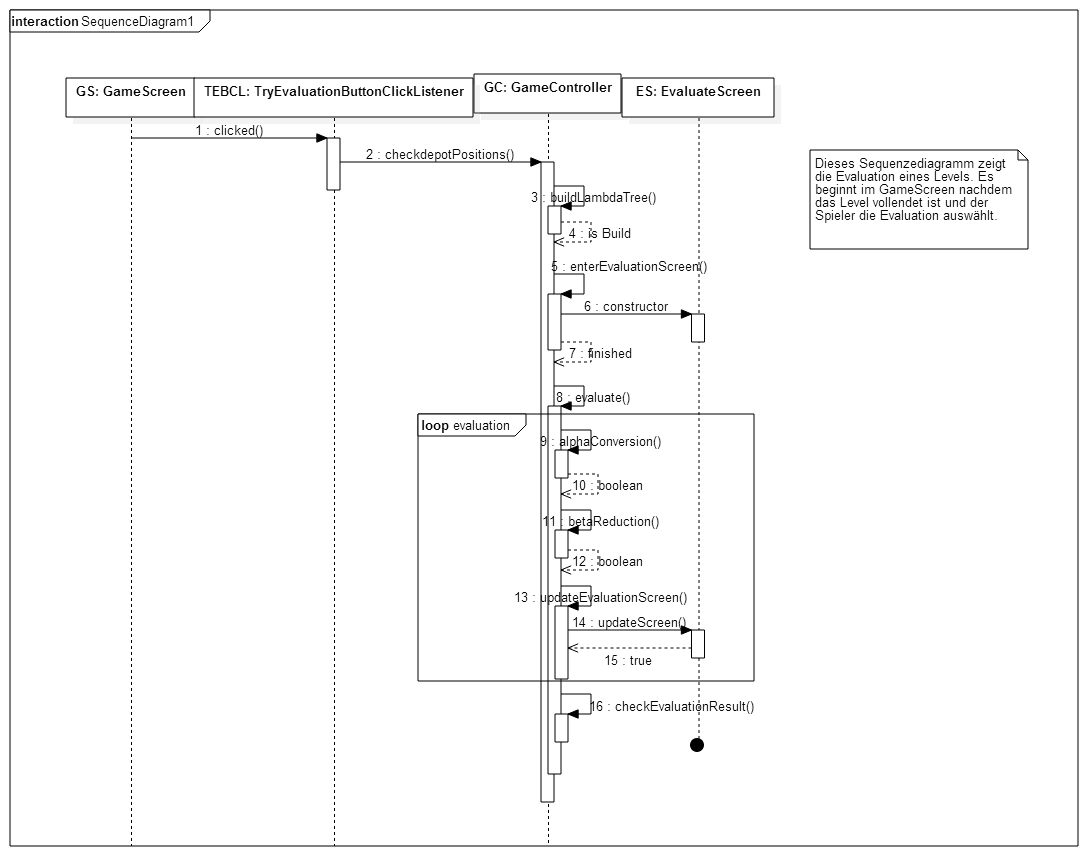
\includegraphics[width=1\textwidth]{../../images/T100Evaluation.png}
    \caption{T100 Evaluation}
    \label{fig:t100evluation}
\end{figure}

\begin{figure}[p]
    \centering
    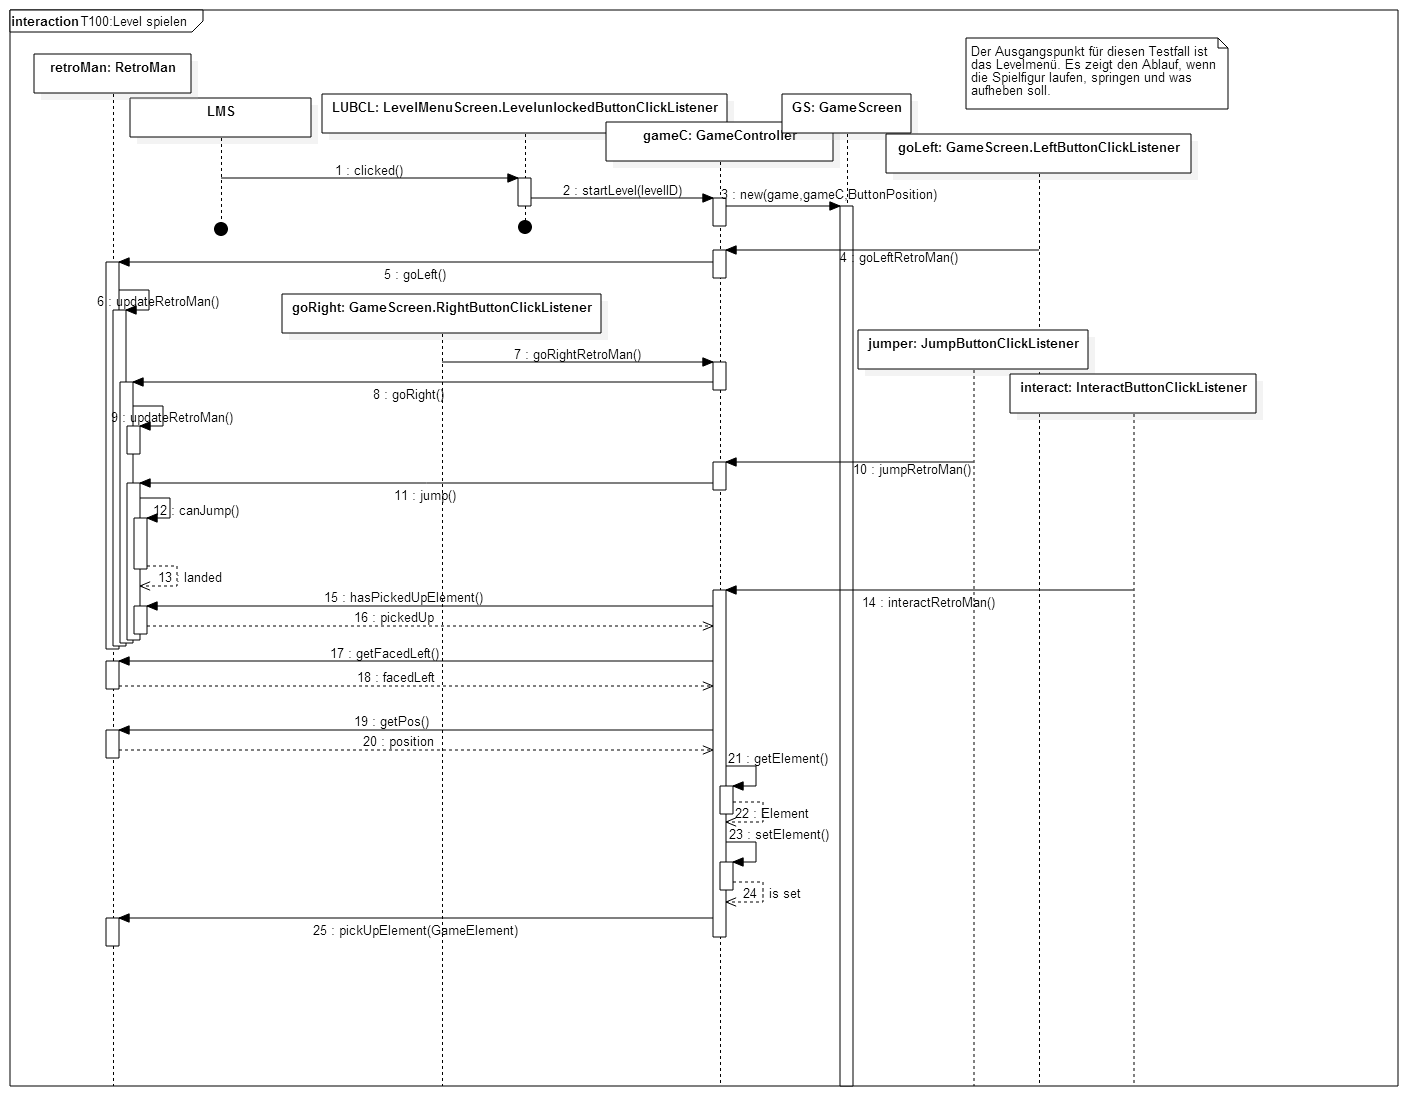
\includegraphics[width=1\textwidth]{../../images/T100_Level_spielen.png}
    \caption{T100 Level spielen}
    \label{fig:t100evluation}
\end{figure}

\begin{figure}[p]
    \centering
    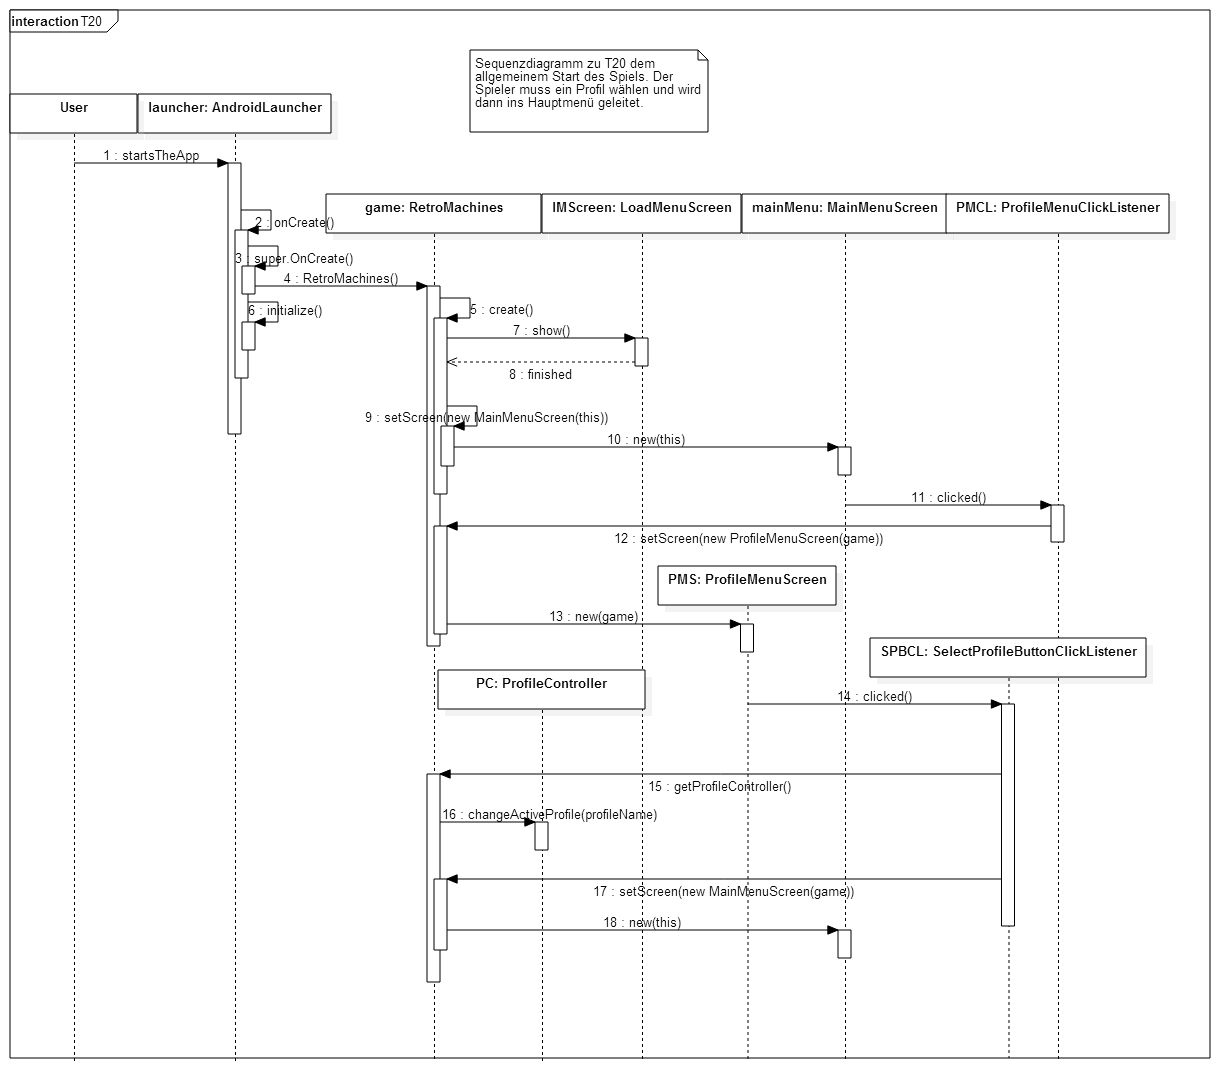
\includegraphics[width=1\textwidth]{../../images/T20.png}
    \caption{T20}
    \label{fig:t100evluation}
\end{figure}

\begin{figure}[p]
    \centering
    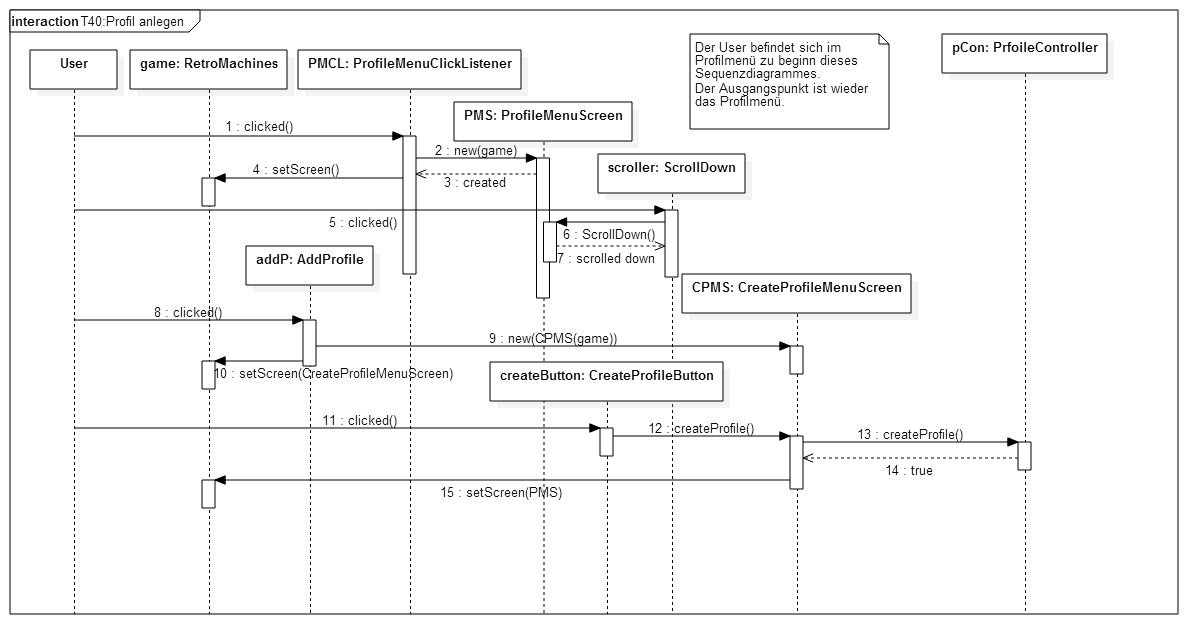
\includegraphics[width=1\textwidth]{../../images/T40_Profil_anlegen.png}
    \caption{T40}
    \label{fig:t100evluation}
\end{figure}

\printindex
\end{document}
